\chapter{MOTION PRIMITIVE TWEAKING:BIPEDAL WALKING}
\label{chap:walk}
\graphicspath{{BipedWalk/BipedWalkFigs/EPS/}{BipedWalk/BipedWalkFigs/}}


The examples of bouncing ball and mass spring systems only illustrate the theory, but have little application value.
This chapter discusses in details about how to adapt a motion primitive for  environmental and application specific constraints.
Combination and transitions of motion primitives are discussed in the next chapter.


The motion primitive understudy in this chapter is \emph{bipedal walking}, which is a topic of great application value for both the graphic and robotic engineering.
In the past decades, many methods have been applied to the bipedal walking, but still we have not achieved  human bipedal walking ability yet.
The early belief is that bipedal walking in nature is unstable, and many control methods are developed based on trajectory following.
The turning point is the discovery of passive dynamic walking machine, which shows under specific conditions, walking needs not control effort.
This idea lead us to believe that walking is an inborn ability, and most problems are solved by the mechanical structure.

In motor invariant theory, bipedal walking is  a motion primitive.
The passive walking gait is treated as the template.
Neural Oscillator and Symmetry Control are applied to tweaking the template while maintaining the global and local motor invariants.
This method generate adaptive gaits and stable gaits in realtime.




\section{Motion Primitives}


For bipedal walking, yaw and roll motion are relative small and usually treated as secondary motion or totally neglected,  main motion happens in the \emph{sagittal plane}, as shown in Figure~\ref{fig:passivekneewalker}
as shown in figure
\begin{figure}[!htbp]
  \begin{center}
    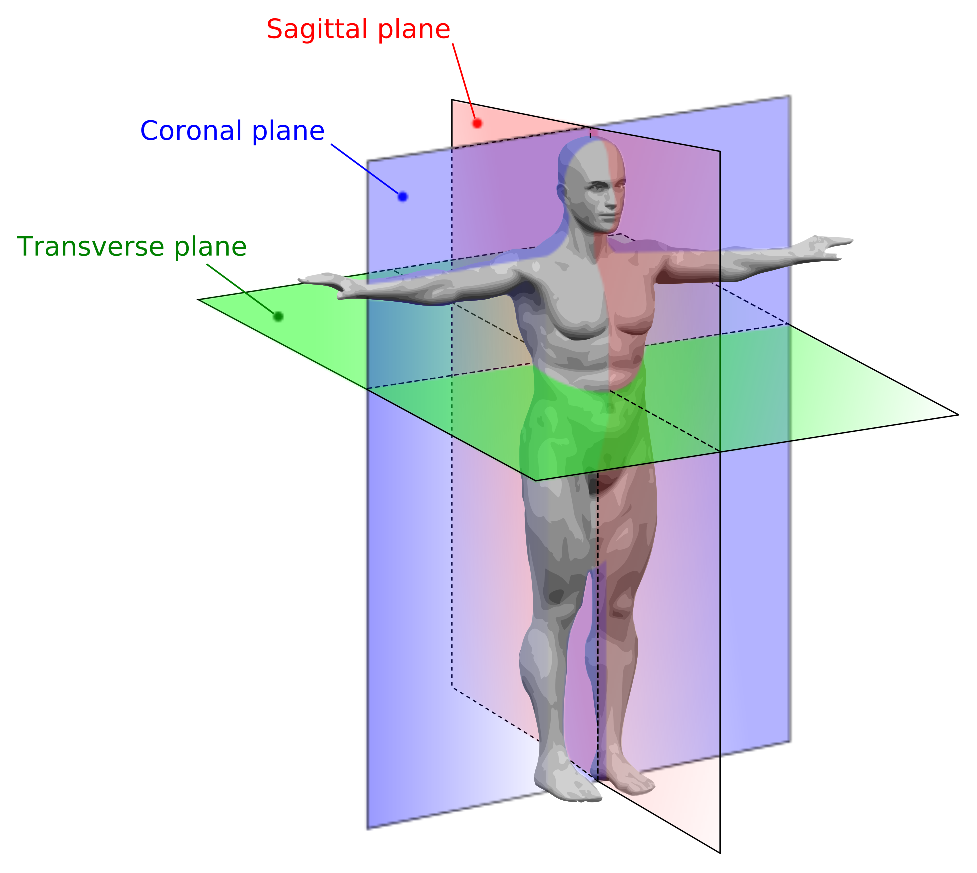
\includegraphics[width=0.7\textwidth]{spahittalPlae}
    \caption{SpahittaPlane}
    \label{fig:passivekneewalker}
\end{center}
\end{figure}




This chapter focuses on the motions in sagittal plane,  \dof s in coronal plane are discussed in Chapter~\ref{chap:highdor}.
More \dof s will introduce perturbations to our model, but will not change the basic motion characteristics and adaptation tendency.
They will make the ``symmetry'' not so perfect and may cause confusions in explaining the idea. thus the discussion is delayed.


The passive walking machine is shown in Figure~\ref{fig:passivekneewalker}.

\begin{figure}[!htbp]
  \begin{center}
    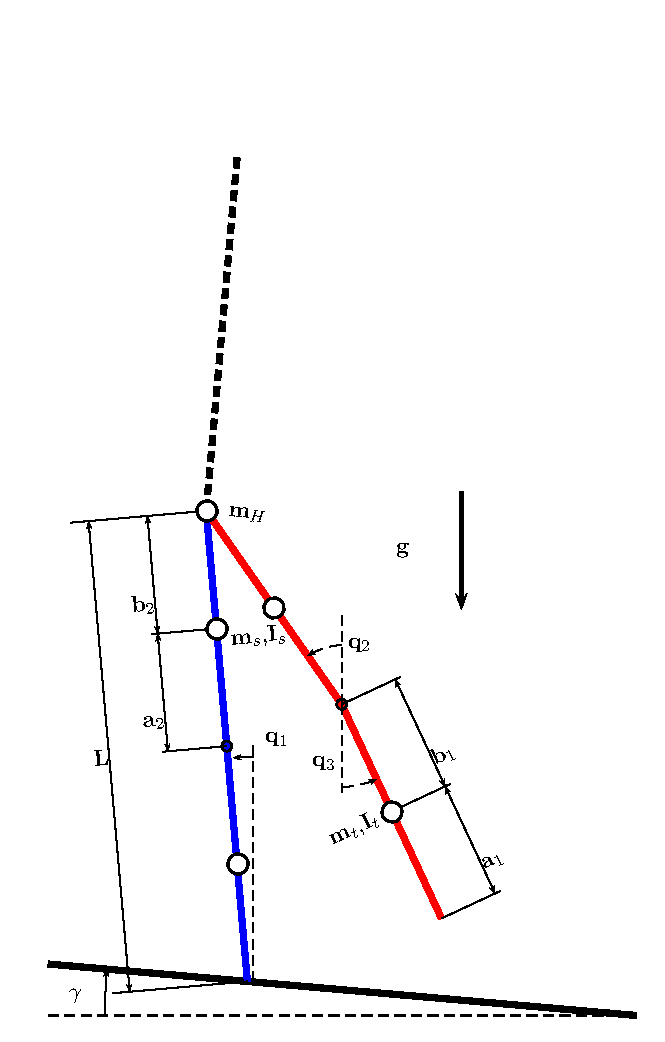
\includegraphics[width=0.7\textwidth]{PWI}
    \caption{A Passive Walking Model with Knee}
    \label{fig:passivekneewalker}
  \end{center}
\end{figure}



\subsection*{Dynamics}

Like the bouncing ball system, this system is hybrid\citep{ames2006categorical}, includes continuous and discrete dynamics[].
Passive walking with knees include four phases\citep{Chen2007}.
\begin{itemize}
\HiItem{Free Swing Phase}
The support leg (the blue one) is kept straight,during this phase the knee of the swing leg is bended, the thigh and shank swings freely.
\HiItem{Knee Strike Phase}
The knee joint of the swing leg has a limit.When the knee angle reach the limit,a collision happens.
After the collision, the swing leg is kept straight.
\HiItem{Knee Lock Swing Phase}
During this swing phase, both the swing and support leg are kept straight.
\HiItem{Heel Strike Phase}
When the heel of the swing leg hits the ground, a collision happens and after that the swing and support legs are switched.
\end{itemize}


The passive walker is modelled based on rigid body dynamics.
Dyanmic equations are developed based on Lagrange Mechanics~\citep{Goldstein2002}.
for details of calculating the dynamic equation, please reference\citep{Chen2007}



\begin{itemize}
\HiItem{Flying Phases}
For both the free and locked knee swing phases are described by the continuous dynamics.
Both equations are in the form of Equation~\ref{eq:flyequation}.
\begin{equation}
\label{eq:flyequation}
M(\mathbf{q}) \ddot{\mathbf{q}} + C(\mathbf{q,\qd})\dot{\mathbf{q}} + N(\mathbf{q}) = 0
\end{equation}
$q=[q_1,q_2,q_3]$,$\qd=[\dot{q_1},\dot{q_2},\dot{q_3}]$
where $M$ is the initial mass matrix, $C$ and $N$ are the centrifugal force matrix and gravity respectively. 
For Free Swing Phase,  $M$ and $C$ are $3$ by $3$ Matrix, $N$ is $3$ by $1$ vector.
for Knee Lock Phase, $M$ and $C$ are $2$ by $2$ Matrix, $N$ is $2$ by $1$ vector.
Put into the standard form, define $\state=[q,\qd]$, Equation~\ref{eq:flyequation} are transformed into Equation~\ref{eq:stateformpw}
Then the function is in the form.
\begin{equation}
\label{eq:stateformpw}
\dot{\state}=
-\left[ 
\begin{array}{cc}
\mathbf{1} &0\\
0 &M 
\end{array}
\right]^{-1}
\left[ 
\begin{array}{cc}
0 &\mathbf{1}\\
0 &C 
\end{array}
\right]\state
-\left[ 
\begin{array}{c}
\mathbf{0}\\
 N 
\end{array}
\right]
\end{equation}

\HiItem{The Strike Phases}
The knee strike and heel strike phases are modelled based on discrete dynamics.
collision equations are developed based on momentum perserving principle.
both collision equations are in the form of Equation~\ref{eq:collidequ}.
\begin{equation}
\label{eq:collidequ}
J^{+}\dot{\mathbf{q}}^{+} = J^{-}\dot{\mathbf{q}}^{-}
\end{equation}

where $J$ is the matrix of angular momentum inetia, the subscripts~$+,-$ represent after and before collision.
For Knees Strike,$J^-$ is a 3 by 2 Matrix, $J^+$ is 2 by 2 Matrix;
For Heel Strike, both $J^{+,-}$ are 2 by 2 Matrix.
\end{itemize}
For the components of each matrix, please refer to the appendix.







With special initial conditions, the passive walker can walk down the slope with a stable gait.
On the phase plot,  a limit cycle emergy. 
Figure ~\ref{fig:phasesmaker} shows the phase plot of one thigh for a stable walking cycle.
Four phases are marked, and Figure~\ref{fig:fwalkingphase} shows the the gait of four phases.

\begin{figure}[!htbp]
  \begin{center}
    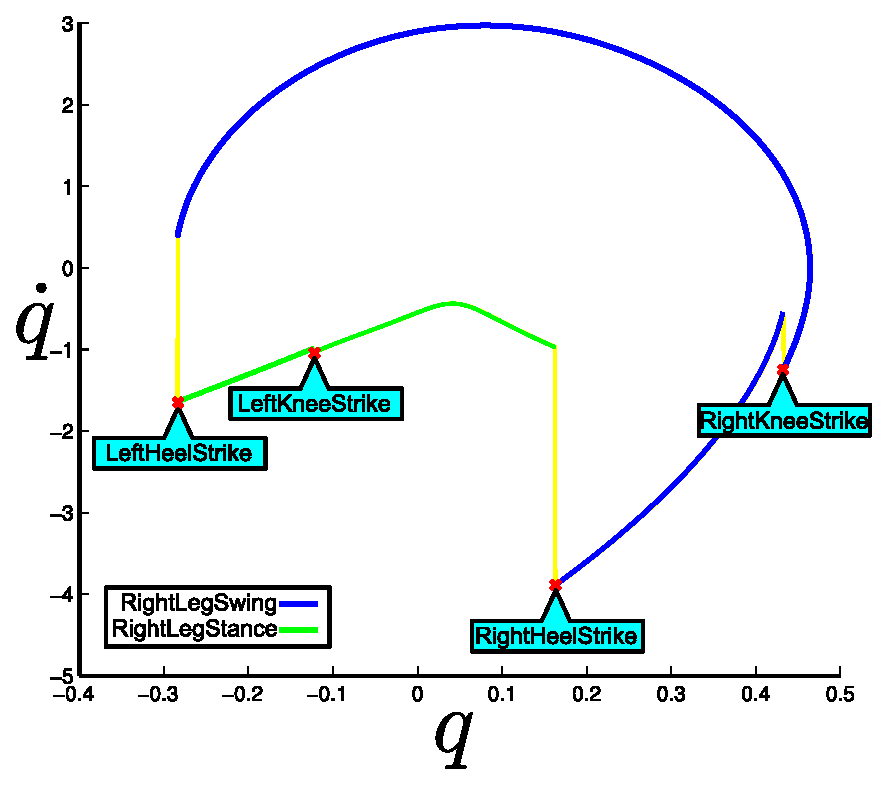
\includegraphics[width=0.7\textwidth]{walk_cycle_index}
    \caption{Four Phases Markered on a Walking Cycle}
    \label{fig:phasesmaker}
\end{center}
\end{figure}

\begin{figure}[!htbp]
  \begin{center}
      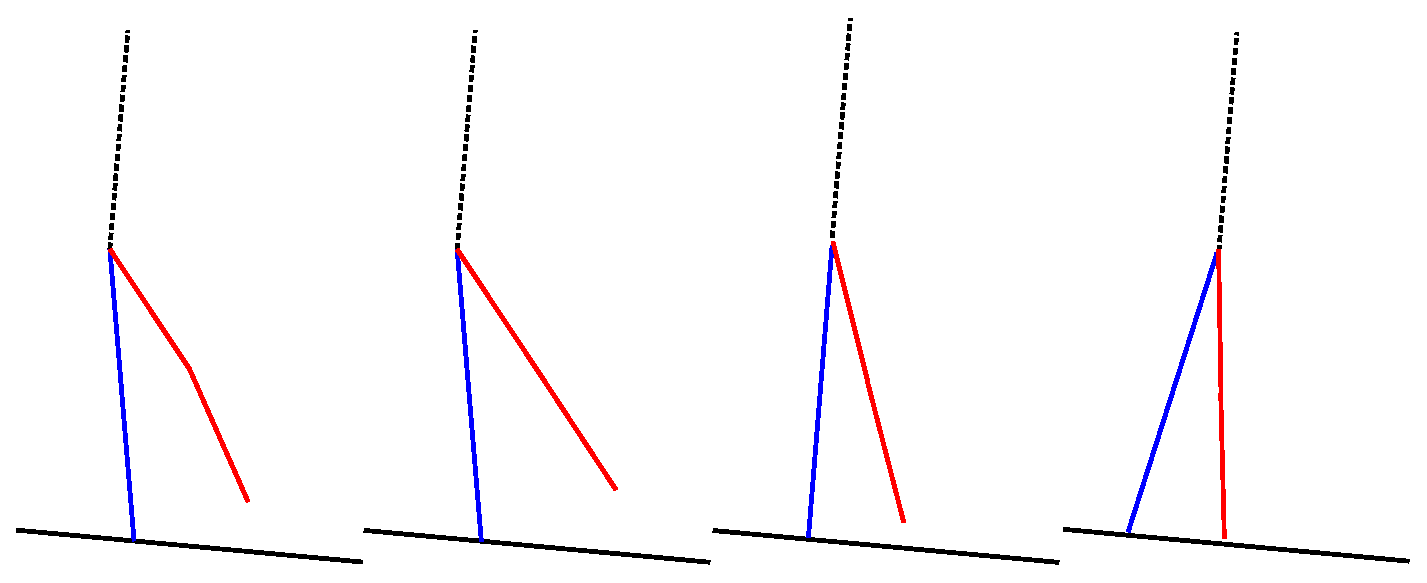
\includegraphics[width=0.7\textwidth]{Fourphase}
    \caption{The four phases in Walking}
    \label{fig:fwalkingphase}
\end{center}
\end{figure}








\section{Global Motor Control and Adaptive Gaits}

\subsection{Entrainment}
Neural oscillator Control  are applied to maintain the stability of limit cycle.

The output of neural oscillator worked as torque applied at hip angel (angle between the two thighs).
The dynamics are shown in Equation~\ref{eq:neuralwalk}
\begin{equation}
\label{eq:neuralwalk}
M(\mathbf{q}) \ddot{\mathbf{q}} + C(\mathbf{q,\qd})\dot{\mathbf{q}} + N(\mathbf{q}) = D\uout
\end{equation}
For the knee lock phase $D=[1,-1]^T$.
For the knee free phase, $D=[1,-1,0]^T$(acting on the difference between the two thighs, not effect the knee)

the input signal is the hip angle,
we have 
\[
	\uin=\hin(q_1-q_2)
\]

when the drive force is small, the limit cycle of entrainment system is similar to the passive one original passive one.
Both limit cycles are shown in Figure~\ref{fig:entrainmentgait} and Figure~\ref{fig:passivegait}.
Walking gatis are shown in Figure




\begin{figure}[!htbp]
  \begin{center}
    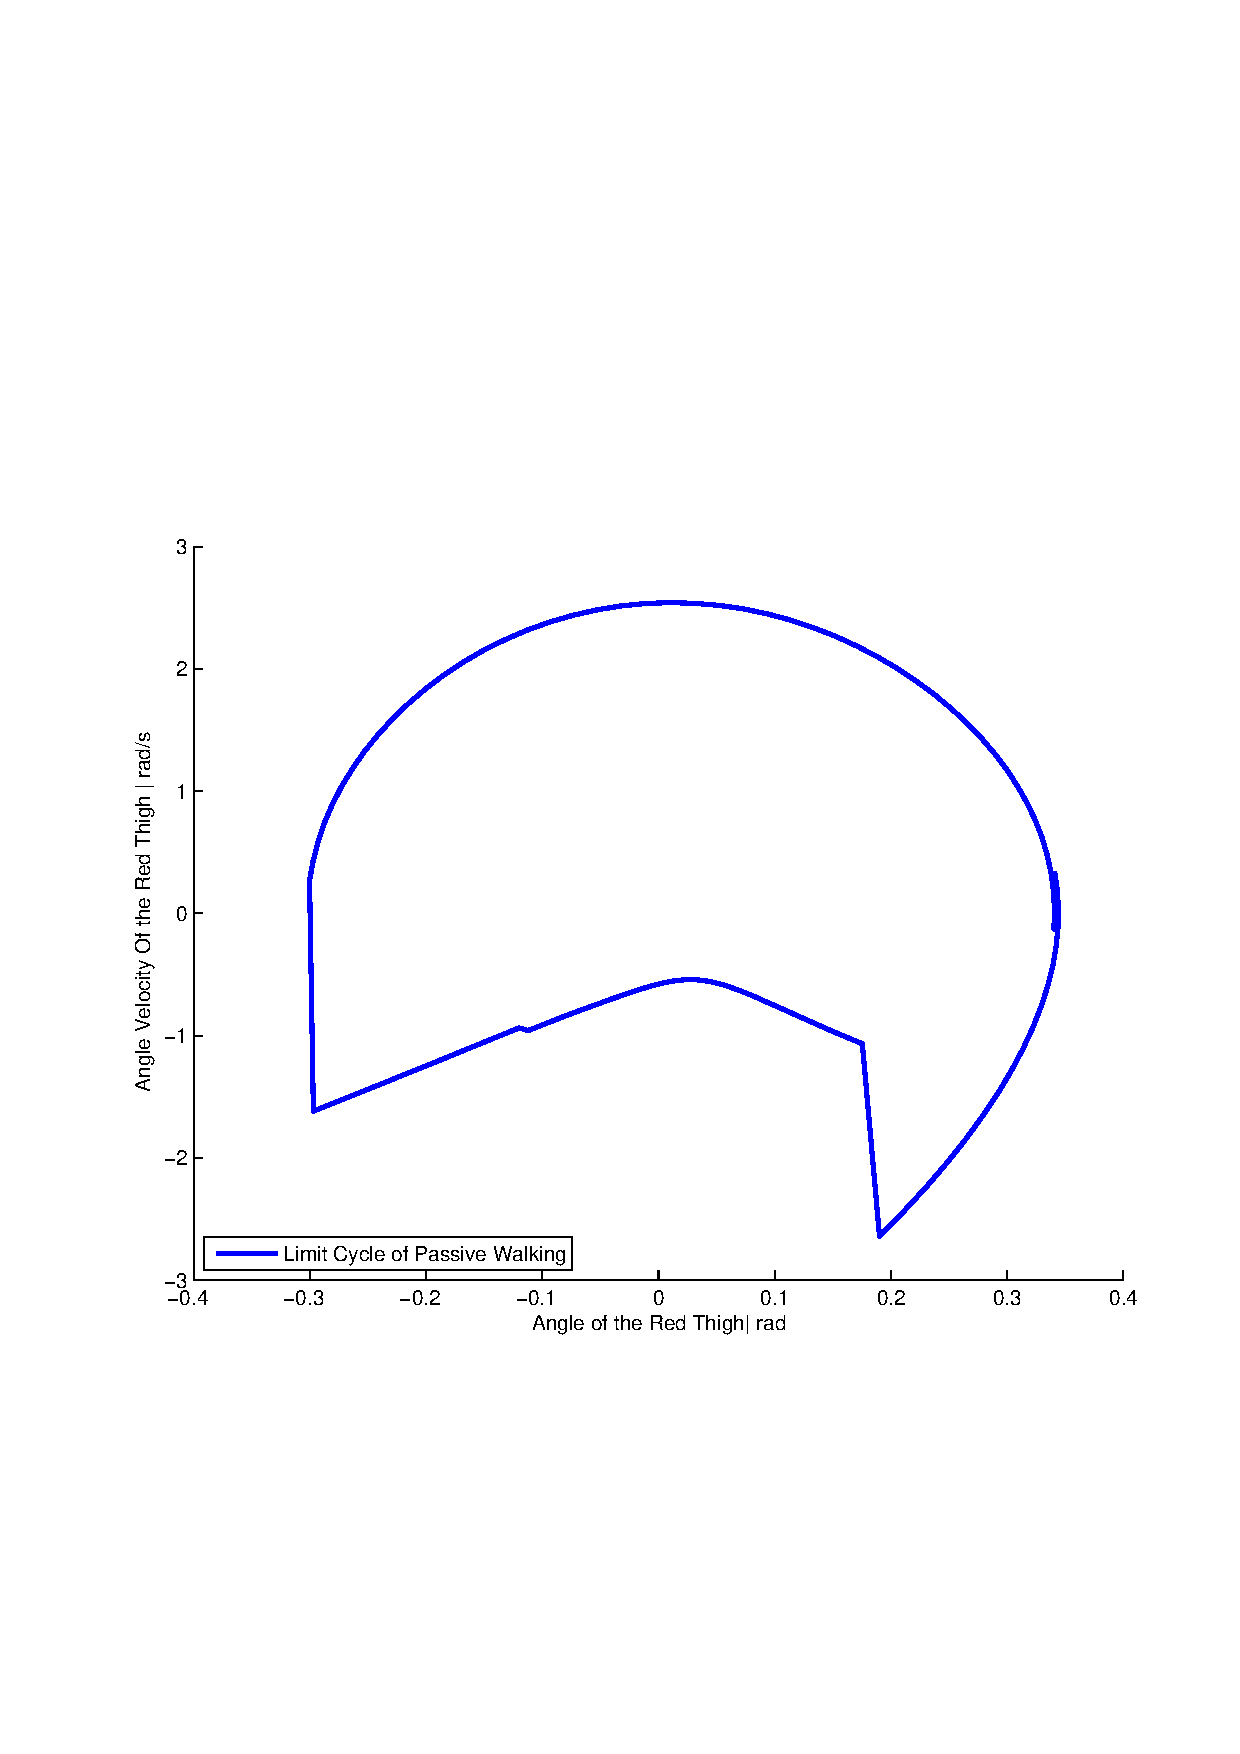
\includegraphics[width=0.7\textwidth]{PassiveWalkingLimitCycle}
    \caption{Limit Circle And Different Phase in Passive Walking}
    \label{fig:passivegaitlimitcycle}
\end{center}
\end{figure}


\begin{figure}[!htbp]
  \begin{center}

      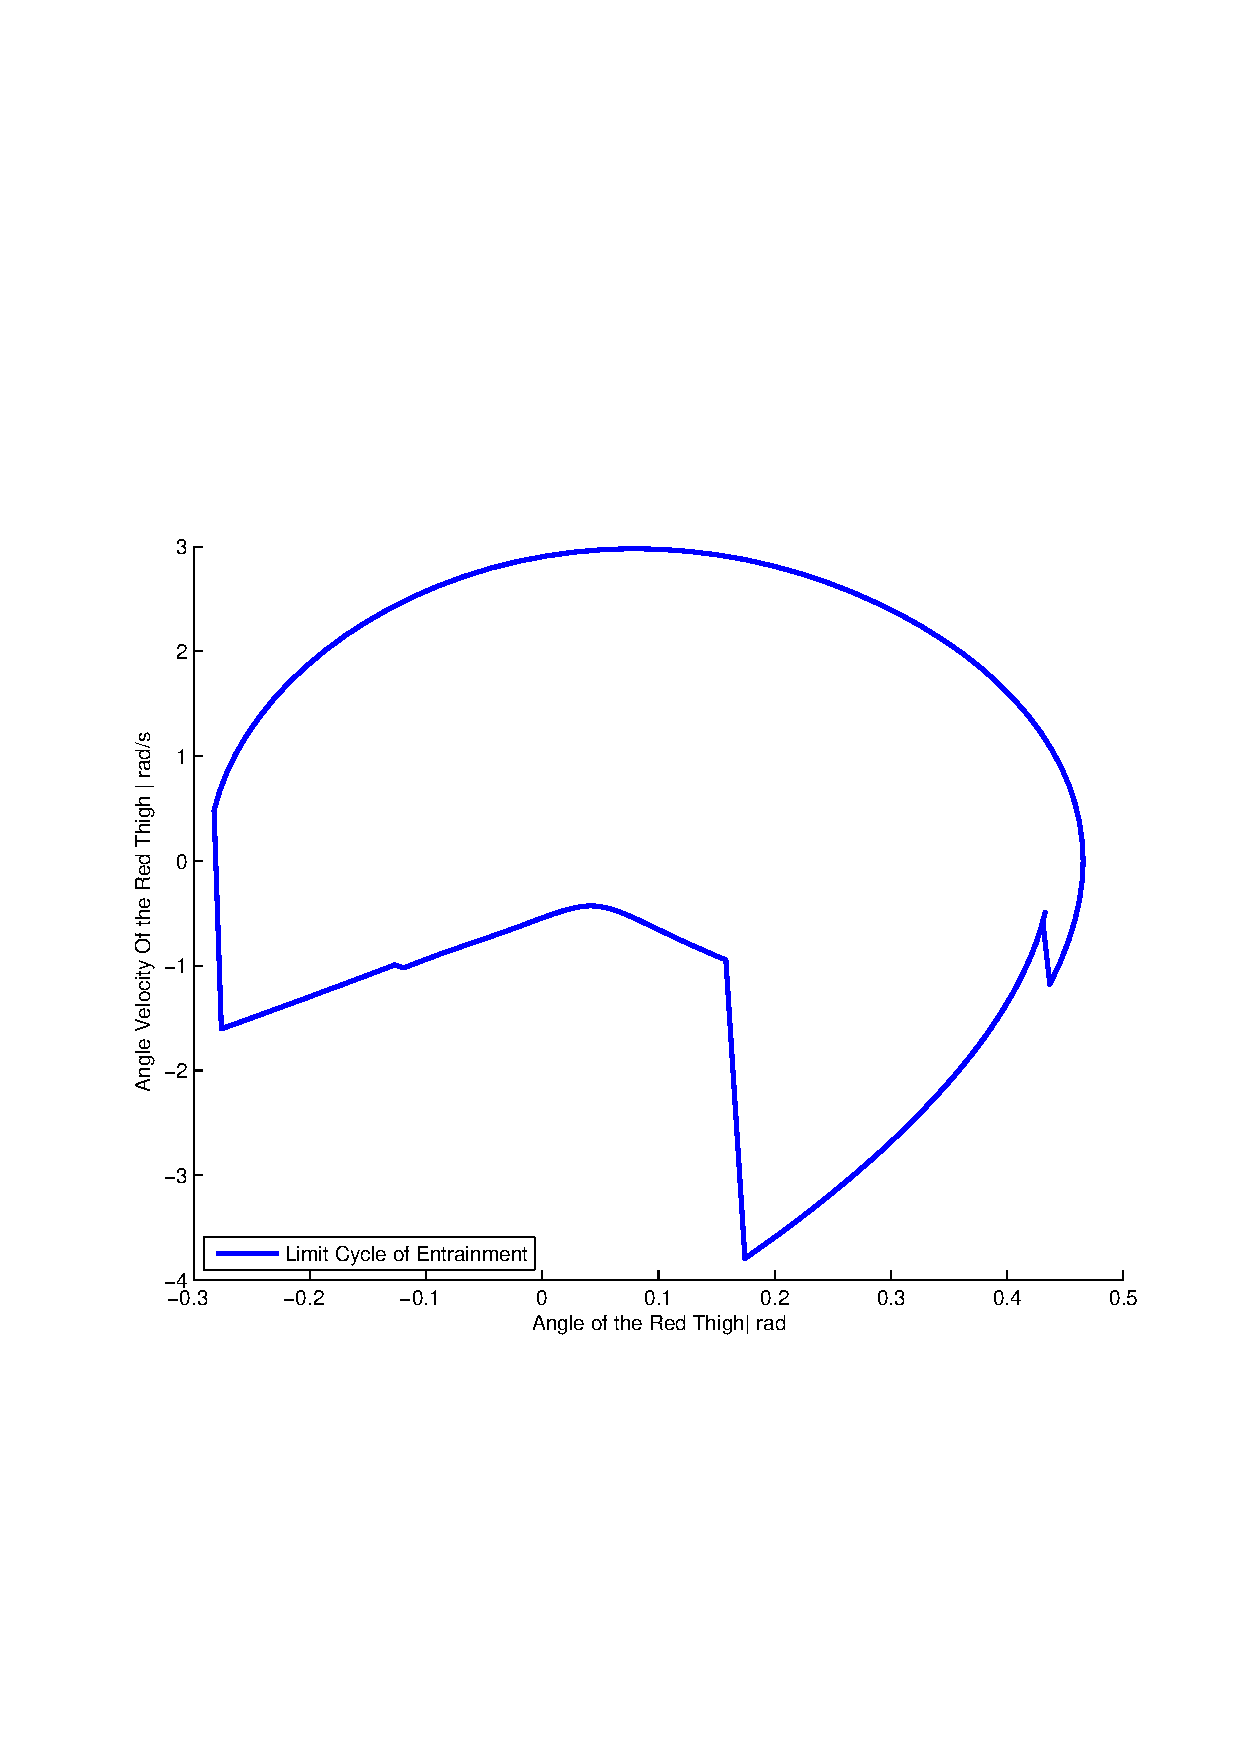
\includegraphics[width=0.7\textwidth]{NeuralWalkingLimitCycle}
    \caption{The gait with neural controller}
    \label{fig:entrainmentgaitlimitcyle}
\end{center}
\end{figure}

\begin{figure}[!htbp]
  \begin{center}
     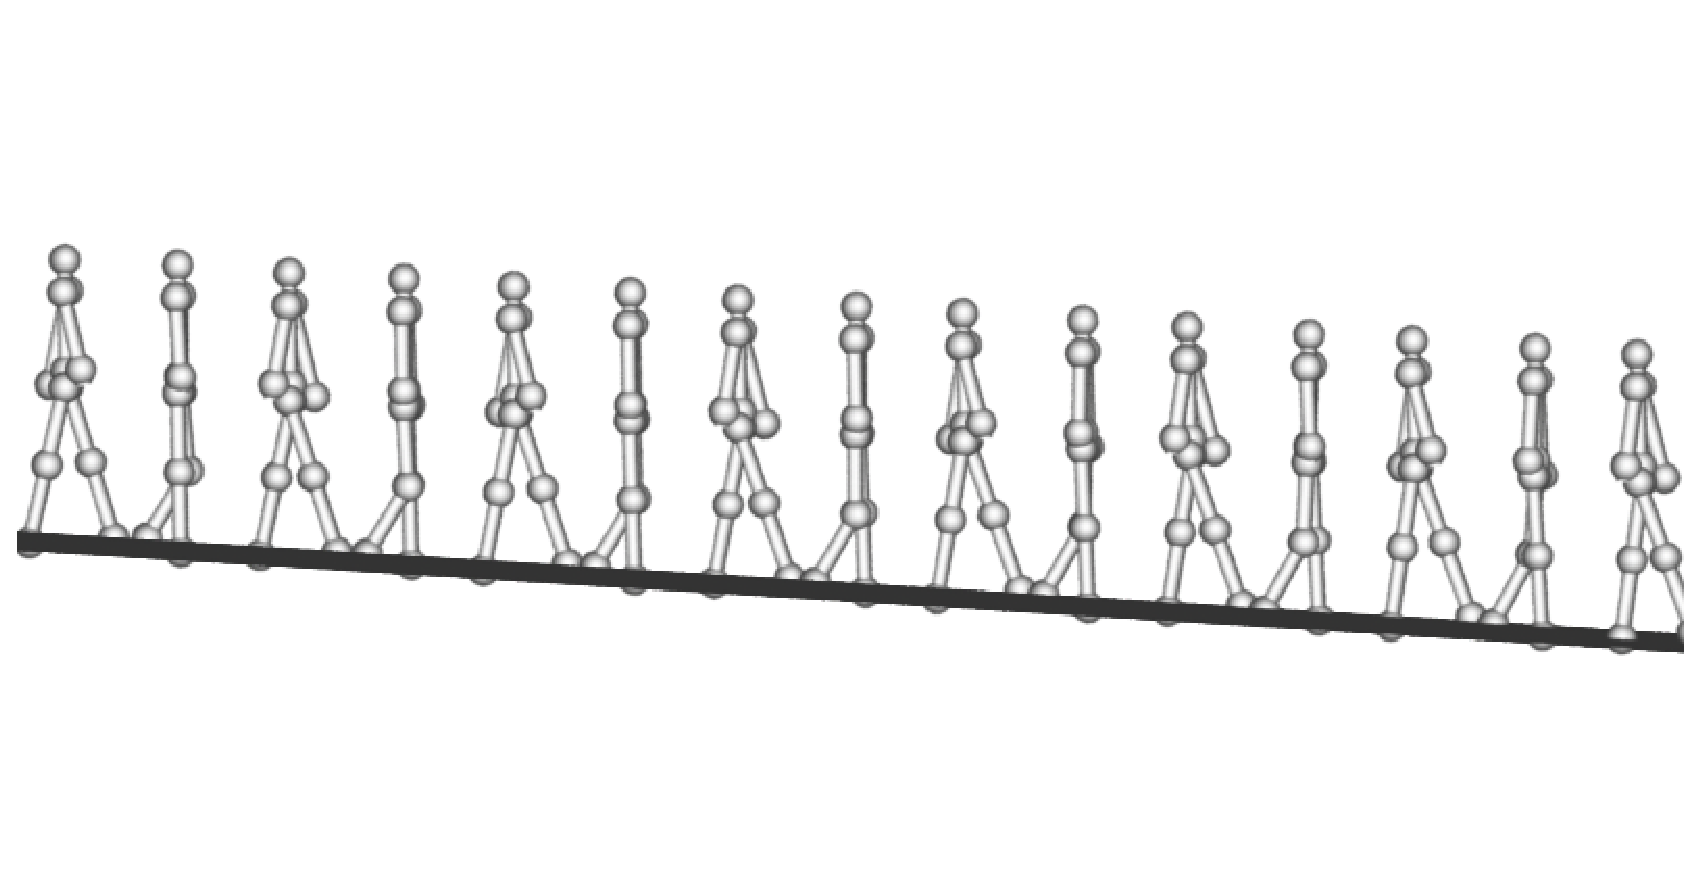
\includegraphics[width=0.7\textwidth]{PassiveGait}
    \caption{The Passive Walking Gait}
    \label{fig:passivegait}
\end{center}
\end{figure}

\begin{figure}[!htbp]
  \begin{center}
     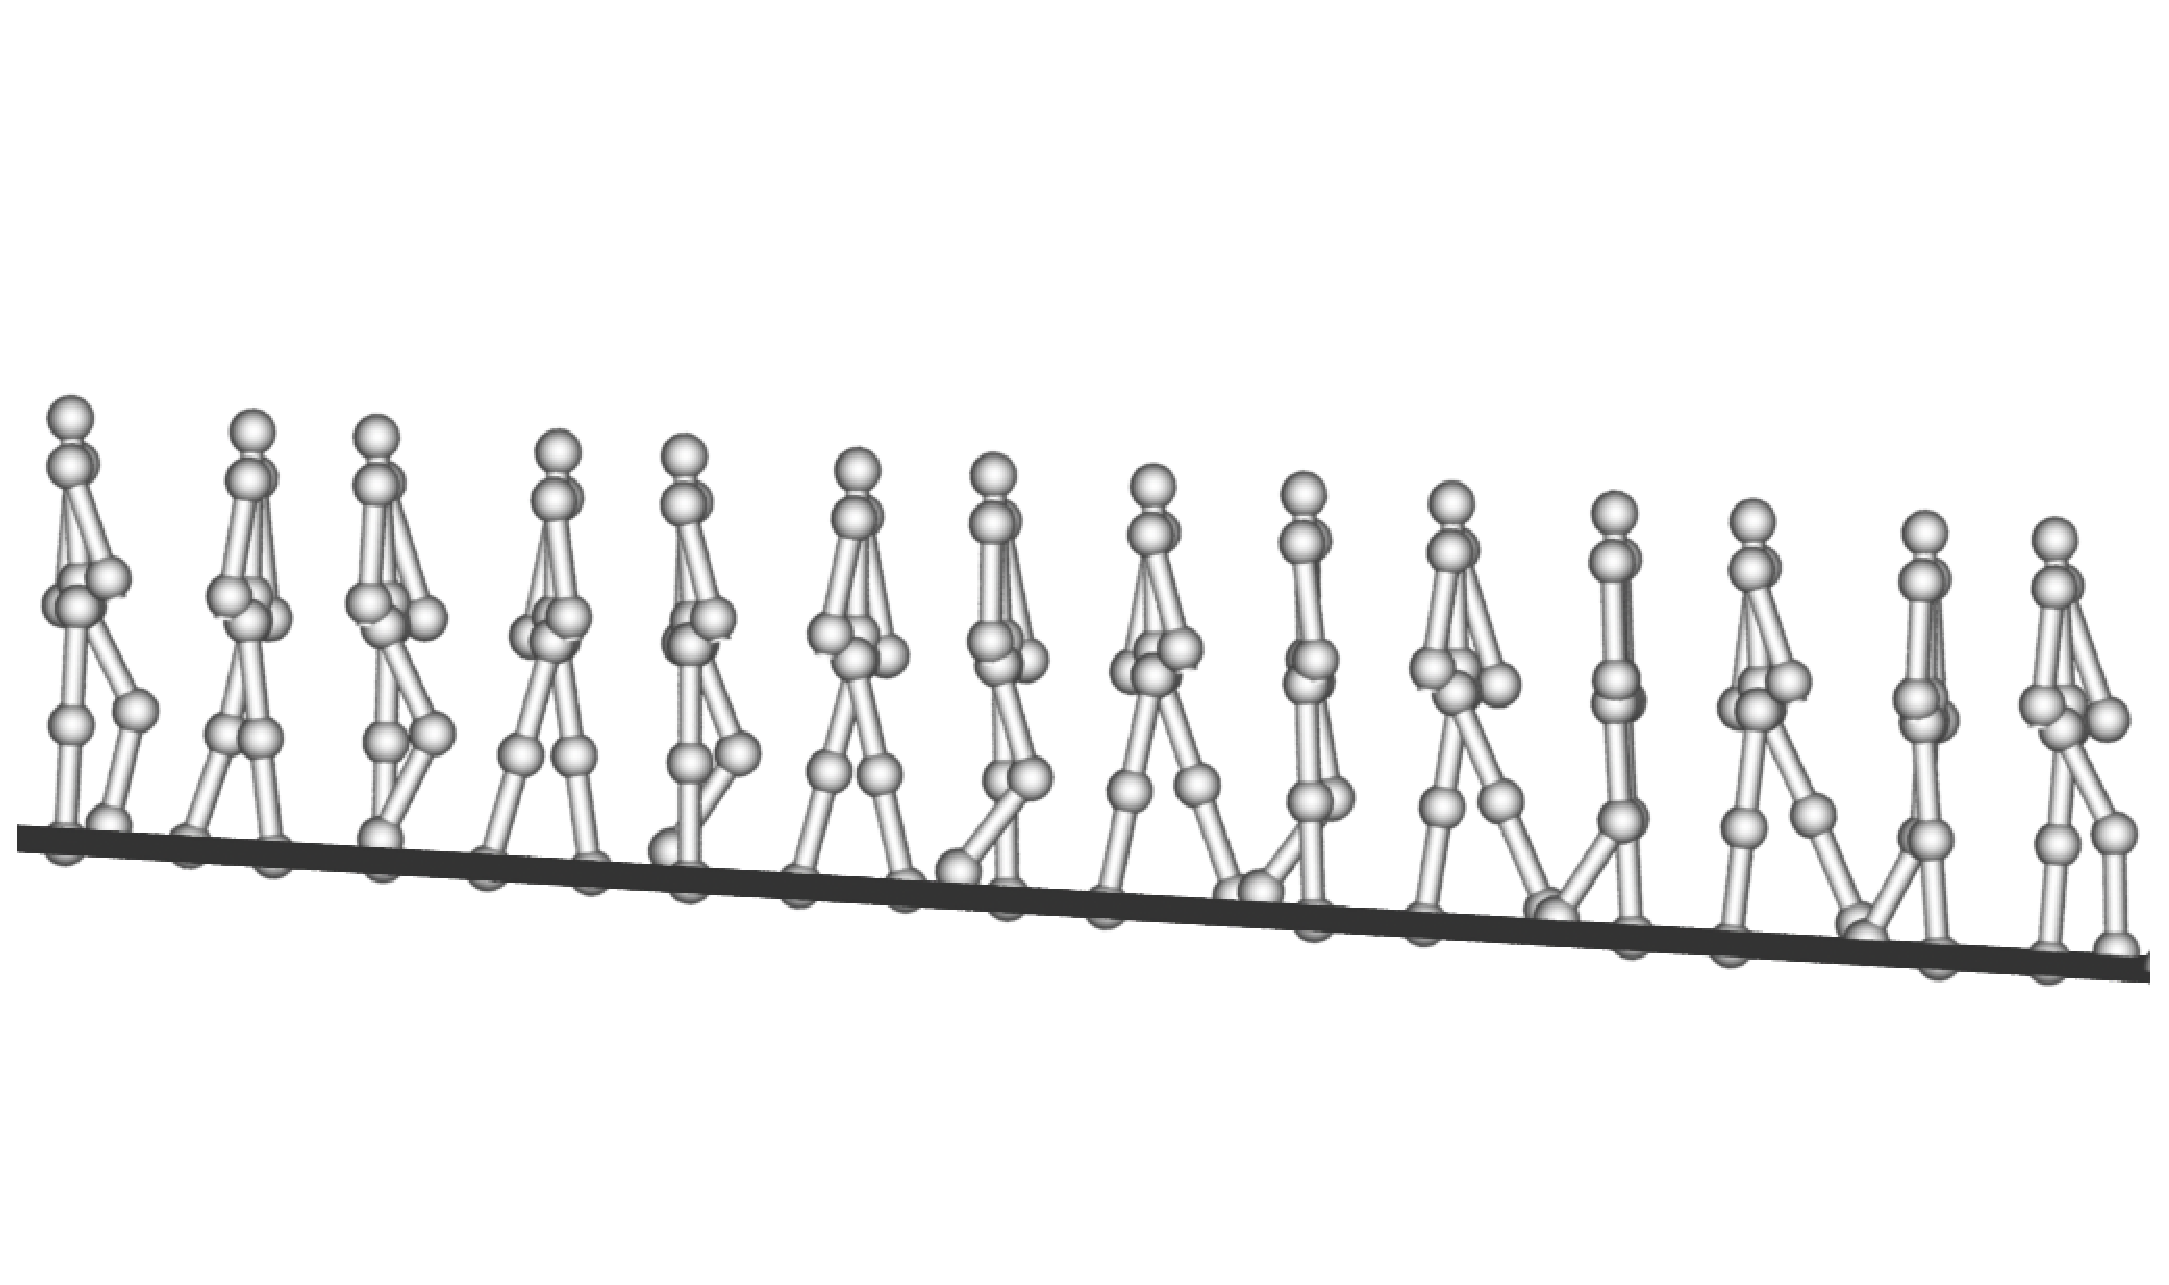
\includegraphics[width=0.7\textwidth]{neuralWalk}
    \caption{Passive Walking with Neural Control}
    \label{fig:entrainmentgait}
\end{center}
\end{figure}



Neural oscillator  boosts structrual stability of walking. 
The passive walking can not be maintained on plane, structure perturbation from slope angle violate the topology, limit cycle does not exist any more.
The stepsize descrease every step, after several steps, and the walker will stop or fall over,as shown in Figure~\ref{fig:passivegaitplane}
After coupling with neural oscillator, the  walker maintain the gait with a small stepsize,as shonw in Figure~\ref{fig:neuralwalkinggait}.
To maintain the energy efficient property of natural motion, $\uout$ is limited to small, thus maintain a small stepsize,as shown in Figure~\ref{fig:entrainmentLimitCycleOnPlane}.

\begin{figure}[!htbp]
  \begin{center}
    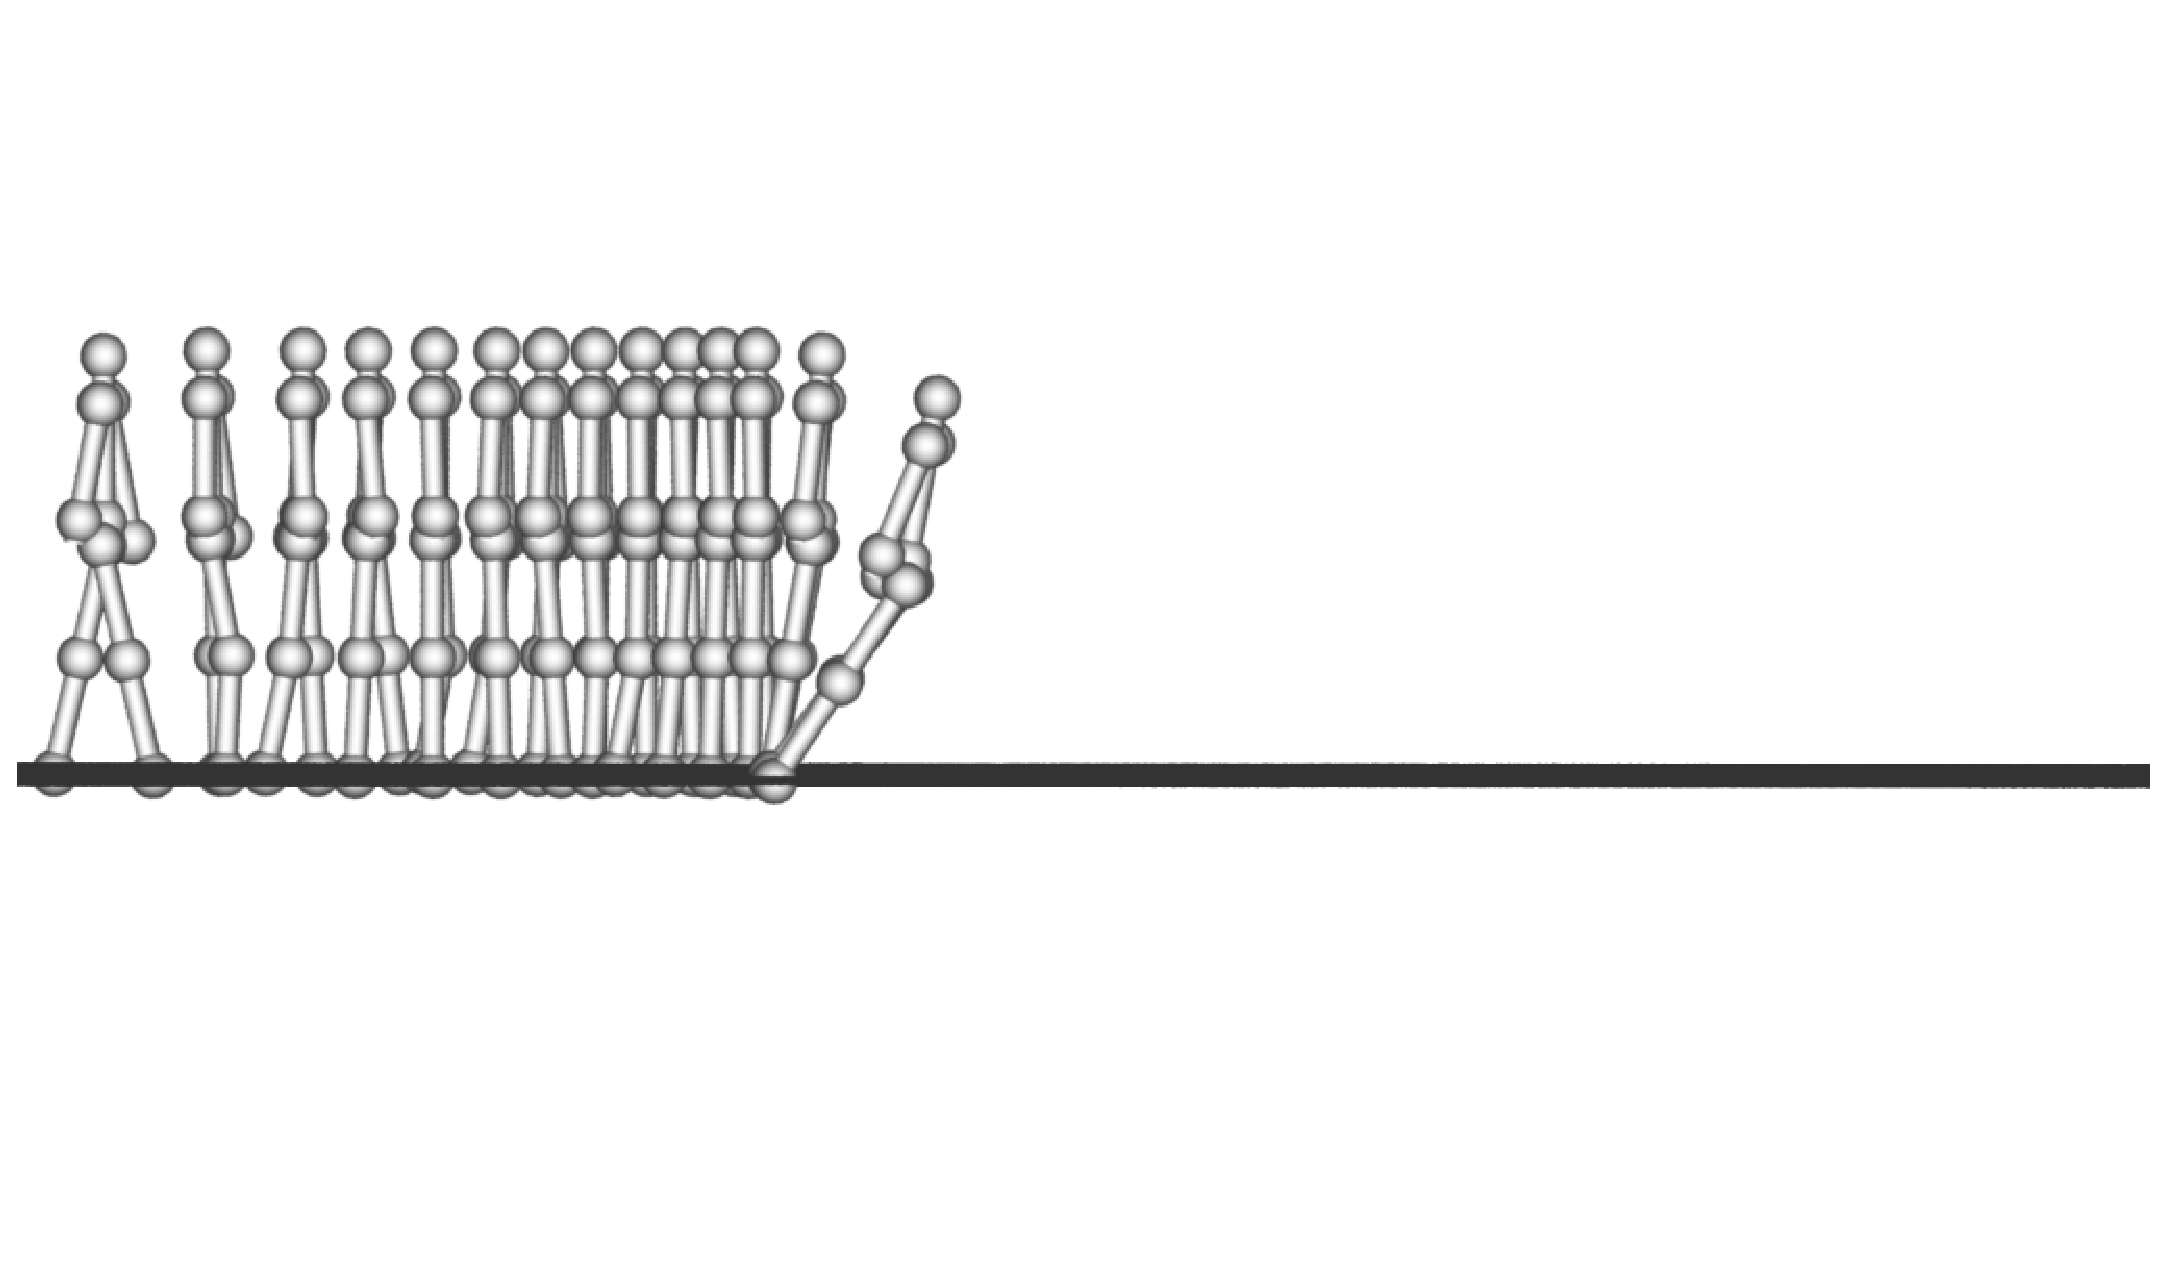
\includegraphics[width=0.7\textwidth]{PassiveOnPlane}
    \caption{Passive On Plain}
    \label{fig:passivegaitplane}
\end{center}
\end{figure}

\begin{figure}[!htbp]
  \begin{center}
     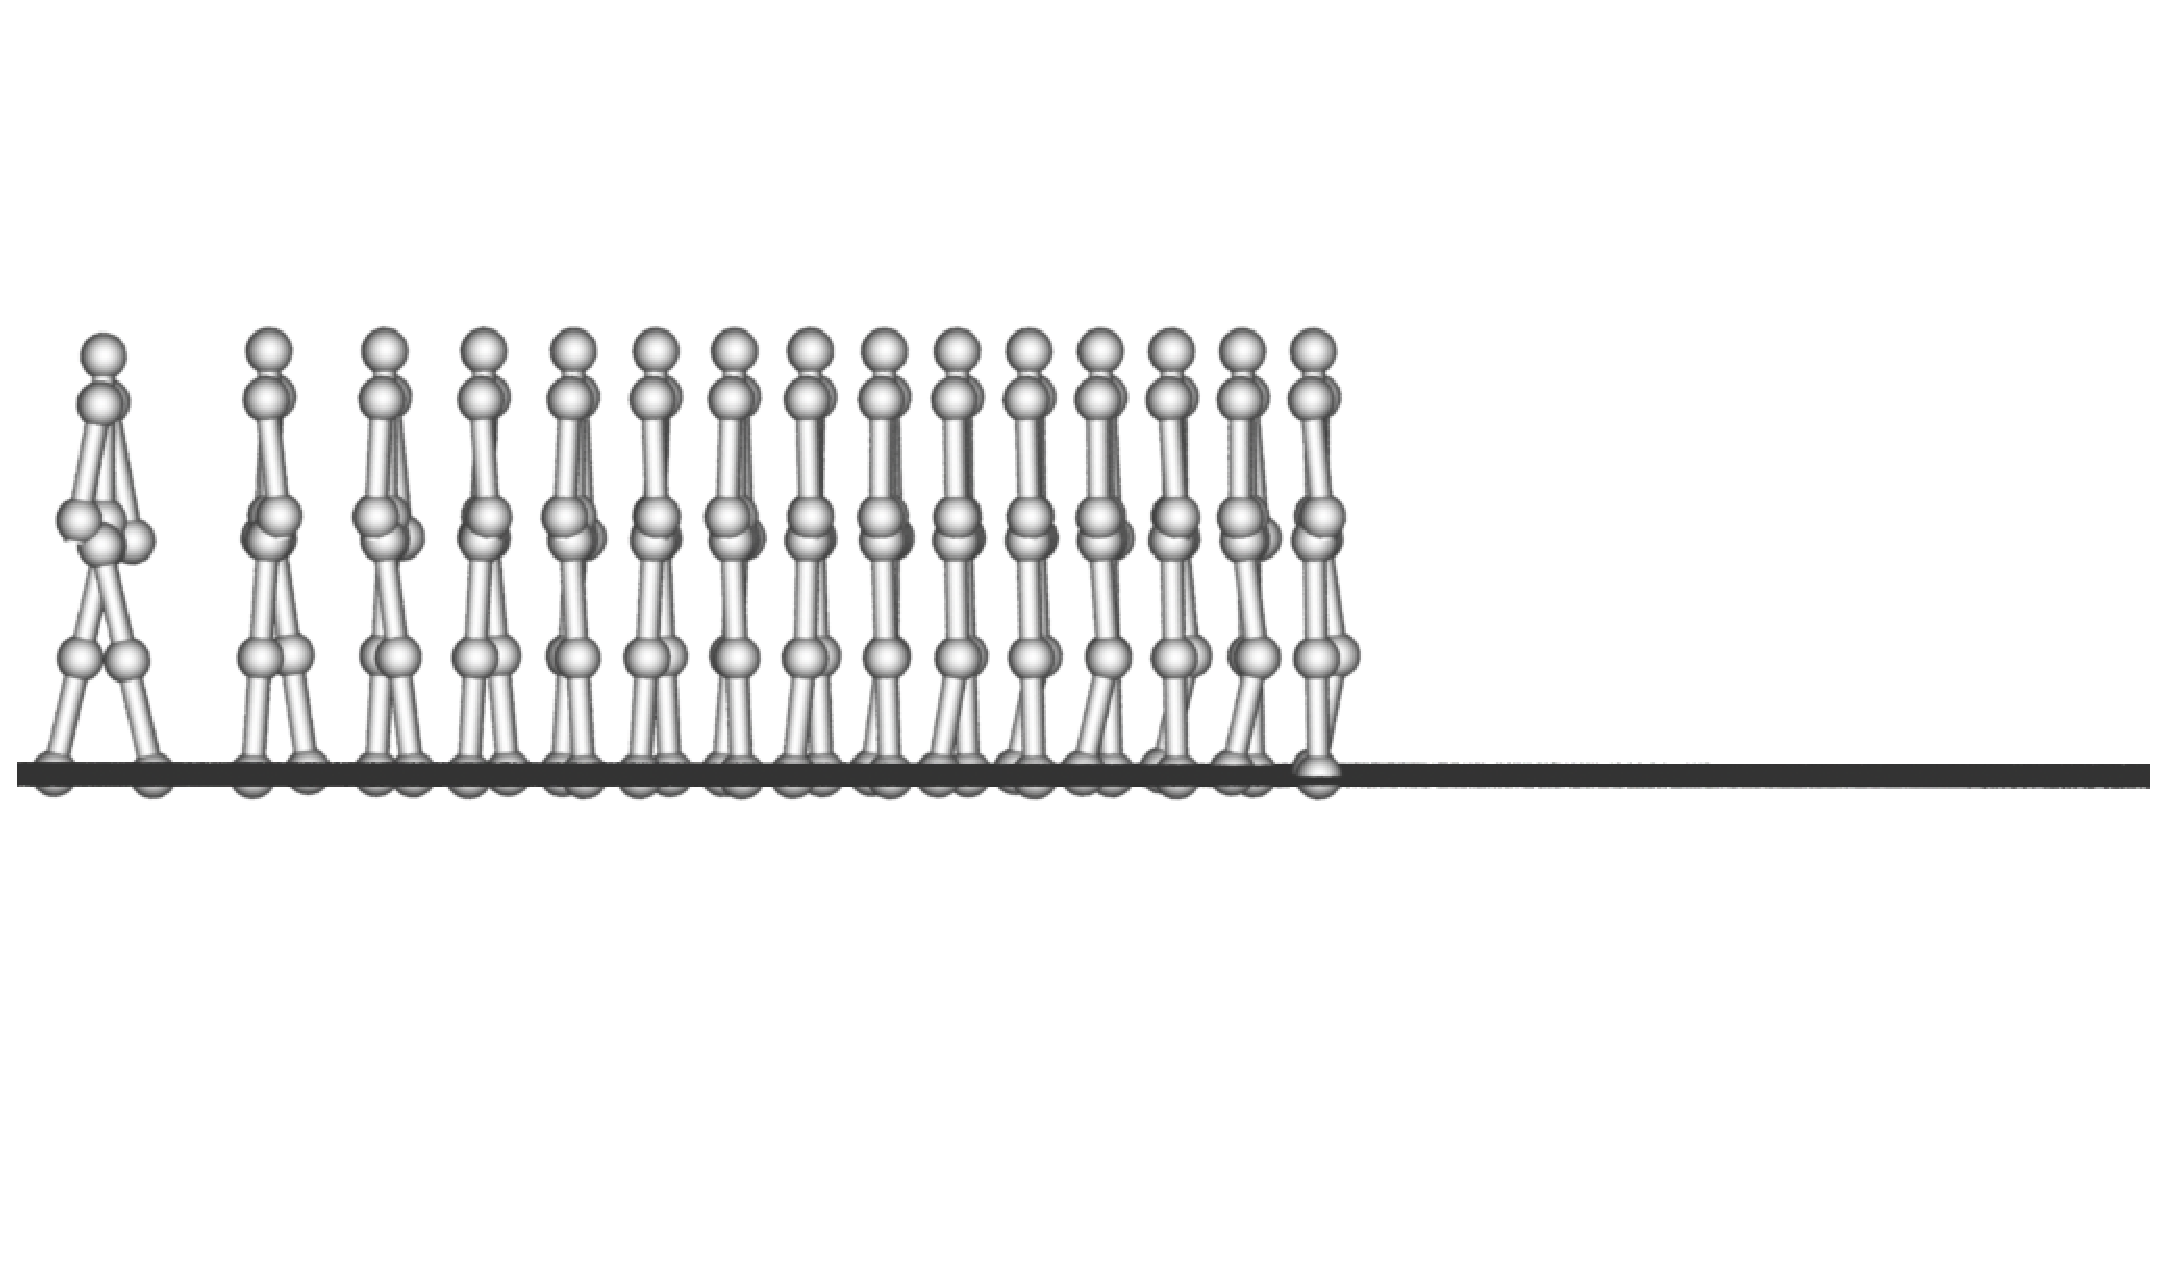
\includegraphics[width=0.7\textwidth]{NeuralWalkingPlane}
    \caption{Entraint Gait On Plane}
    \label{fig:neuralwalkinggait}
\end{center}
\end{figure}

\begin{figure}[!htbp]
  \begin{center}
      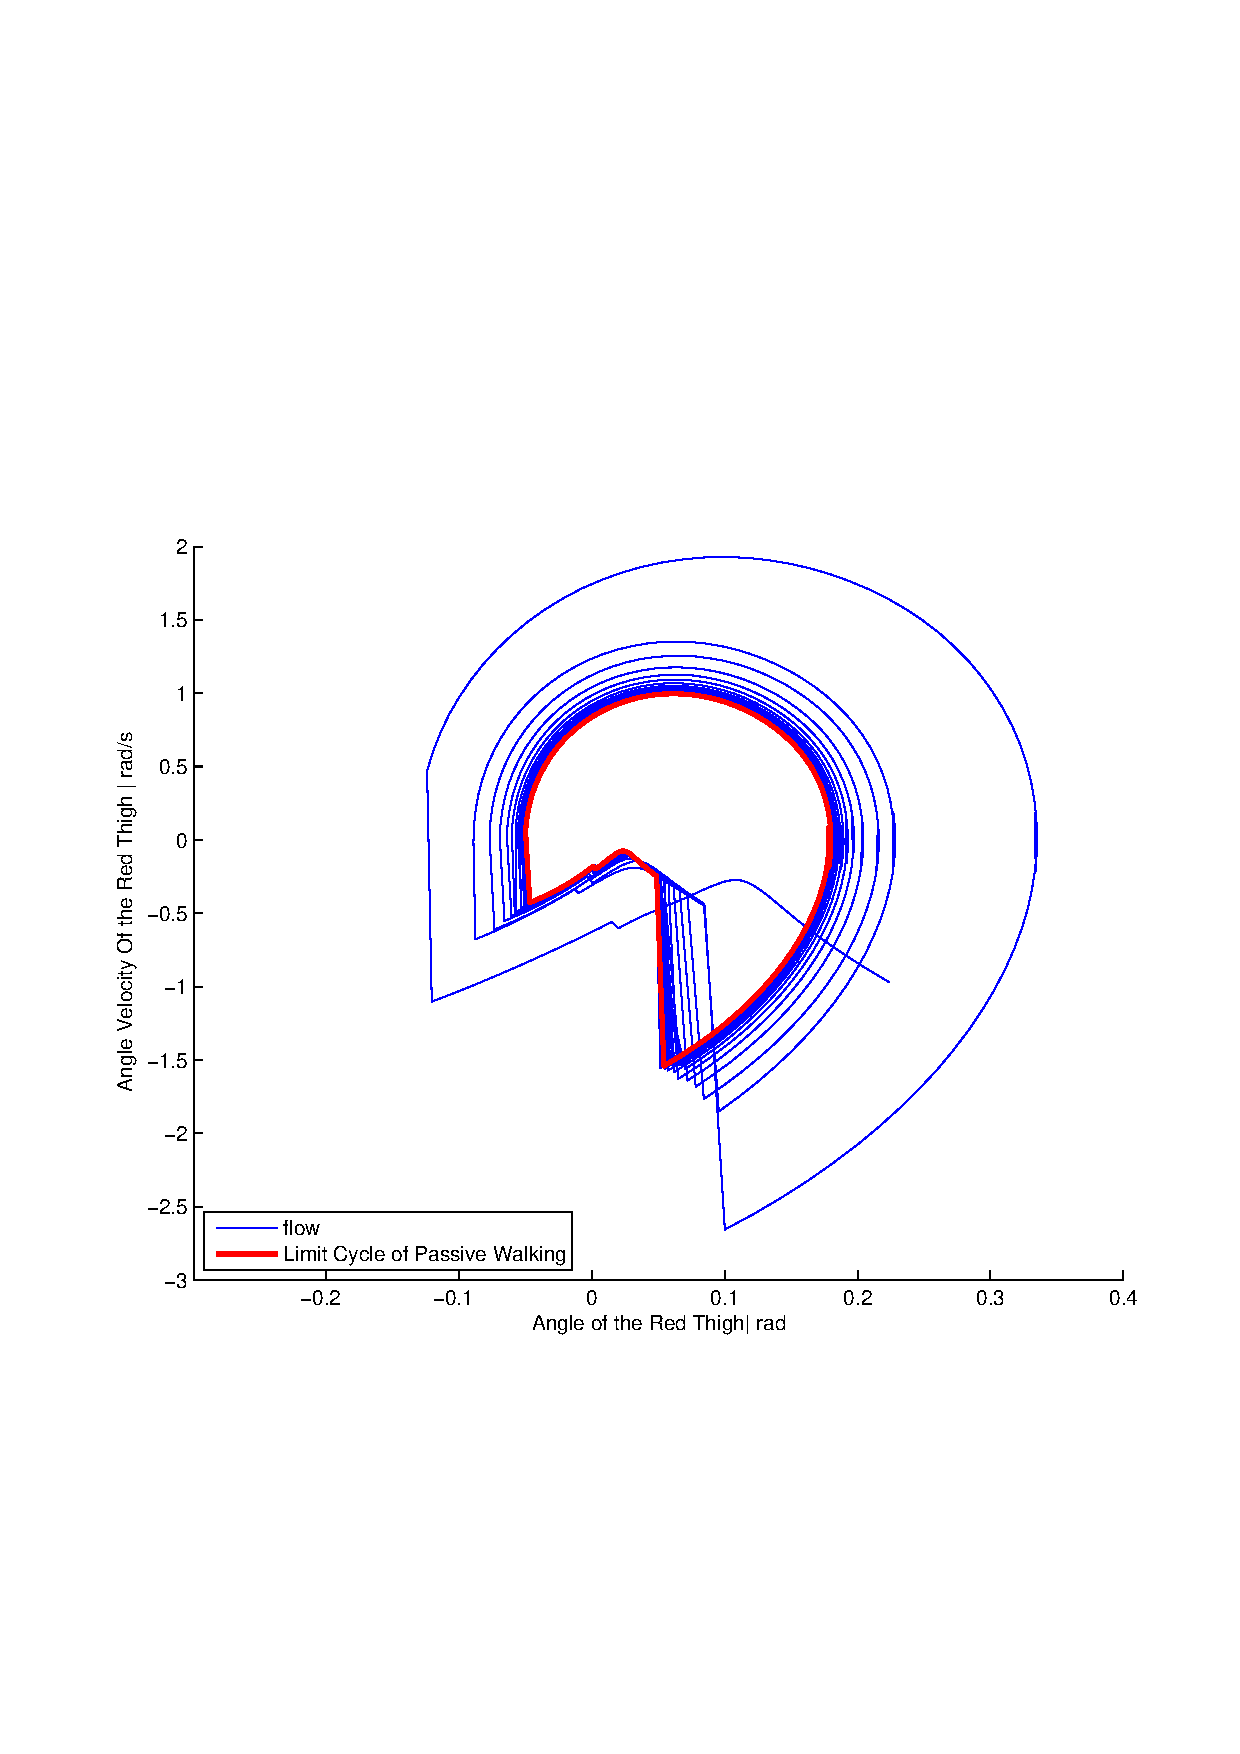
\includegraphics[width=0.7\textwidth]{NeuralPlaneCycle}
    \caption{Limit Cycle of entrainment gait on plane}
    \label{fig:entrainmentLimitCycleOnPlane}
\end{center}
\end{figure}



For Figure~\ref{fig:entrainmentLimitCycleOnPlane}, the initial postion is far from the limit cycle, this shows that the basin of attraction has been enlarged.
State perturbation applied to generate pushed or pulled walking gaits as shown in Figure~\ref{fig:PushGait} and Figure~\ref{fig:PullGait}.
And Figure~\ref{fig:PushGaitPlot} and Figure~\ref{PullGaitPhasePlot}.

\begin{figure}[!htbp]
  \begin{center}
      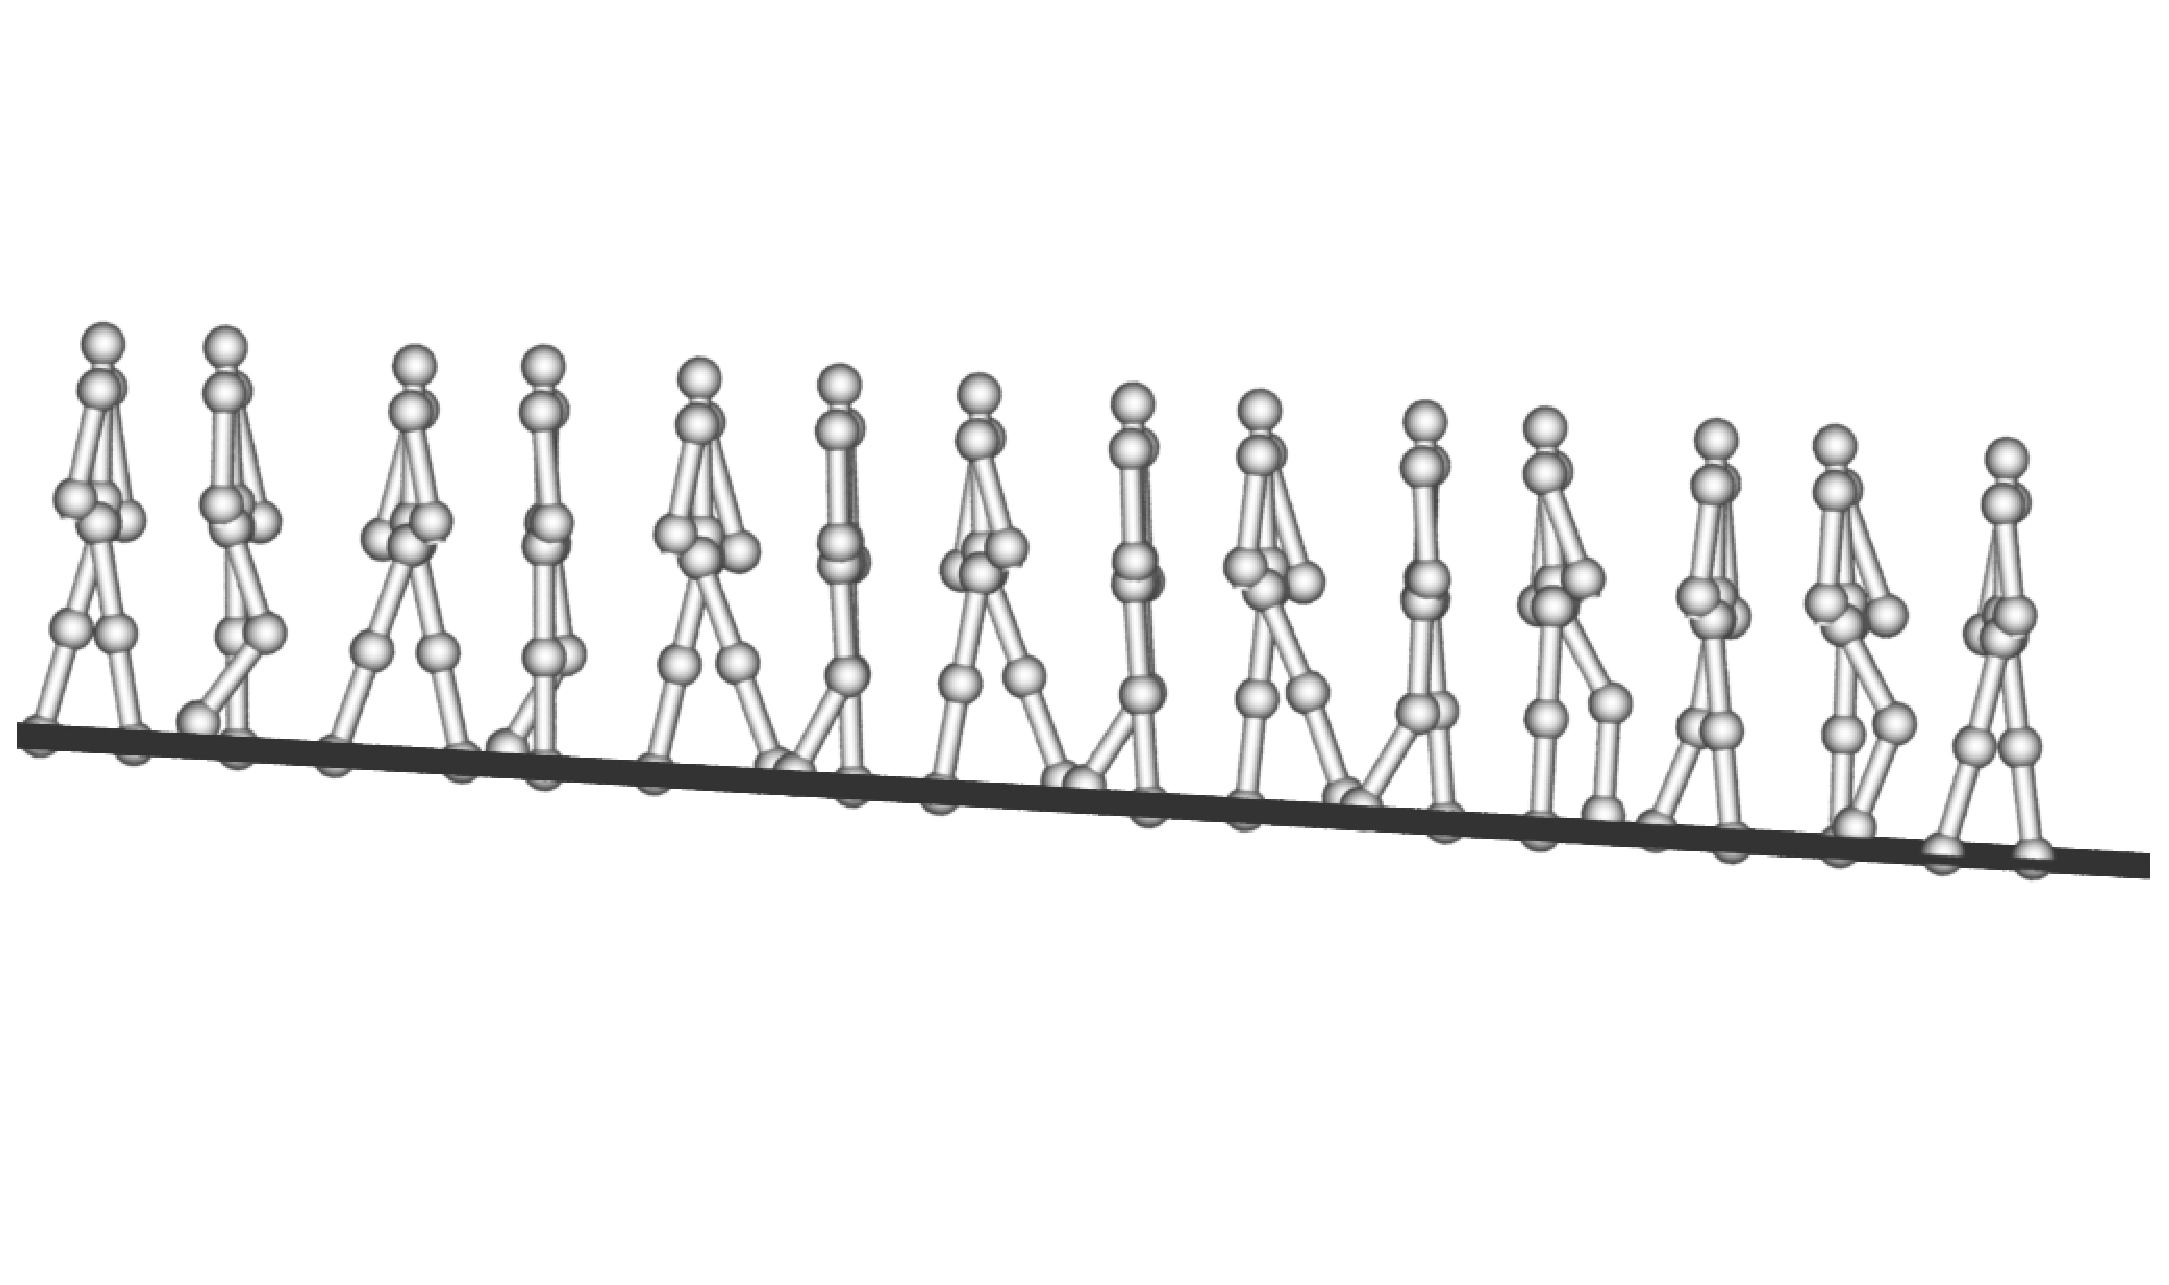
\includegraphics[width=0.7\textwidth]{PushGait}
    \caption{The Push Perturbated Gait}
    \label{fig:PushGait}
\end{center}
\end{figure}


\begin{figure}[!htbp]
  \begin{center}
      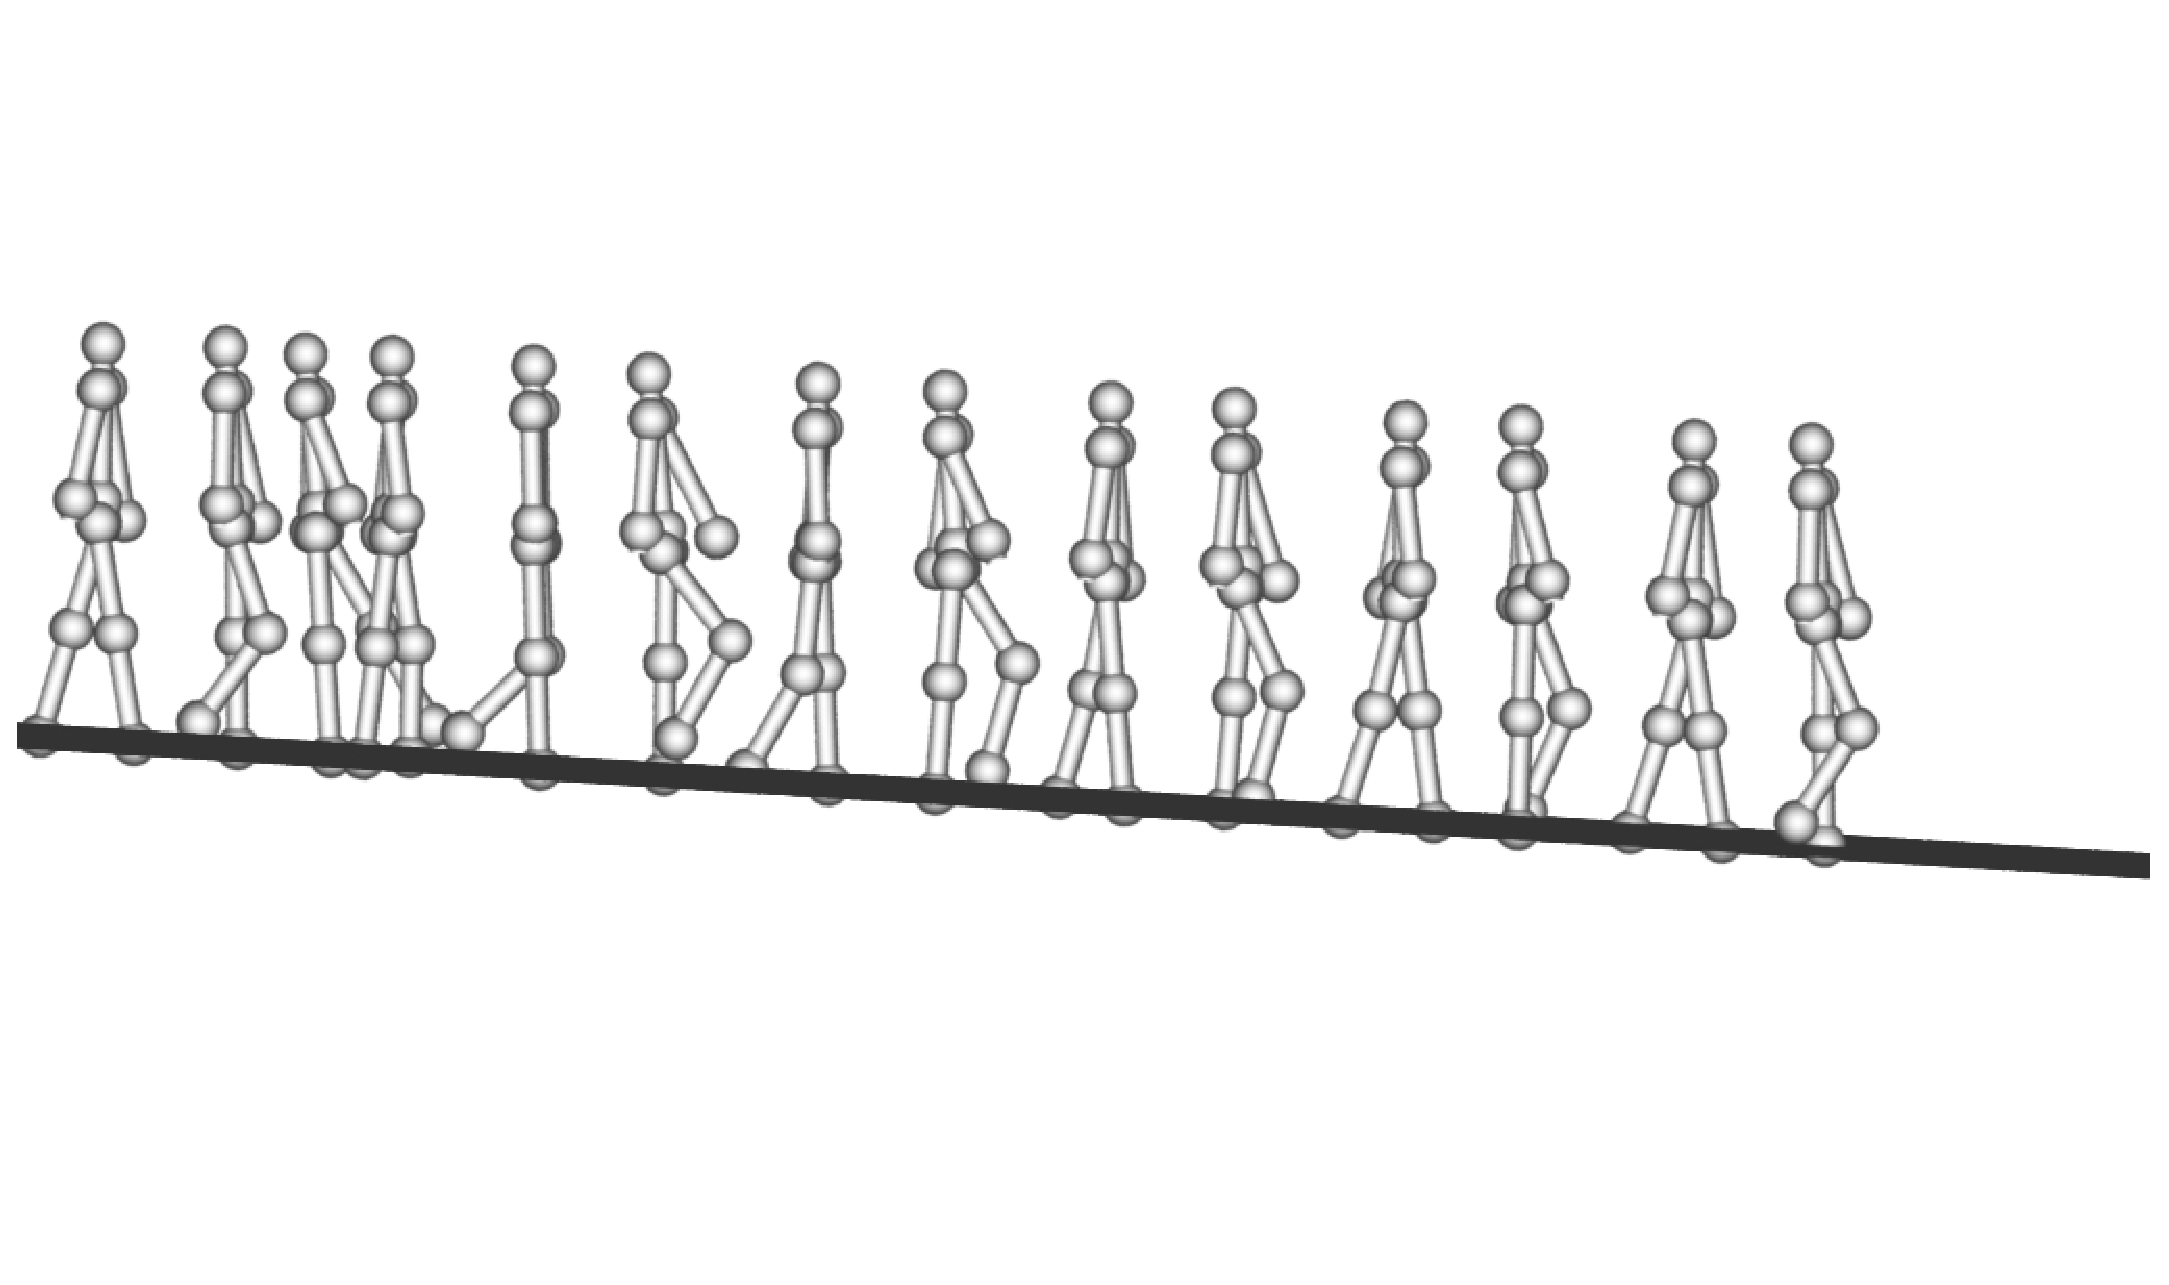
\includegraphics[width=0.7\textwidth]{PullGait}
    \caption{The Pull Perturbated Gait}
    \label{fig:PullGait}
\end{center}
\end{figure}


\begin{figure}[!htbp]
  \begin{center}
      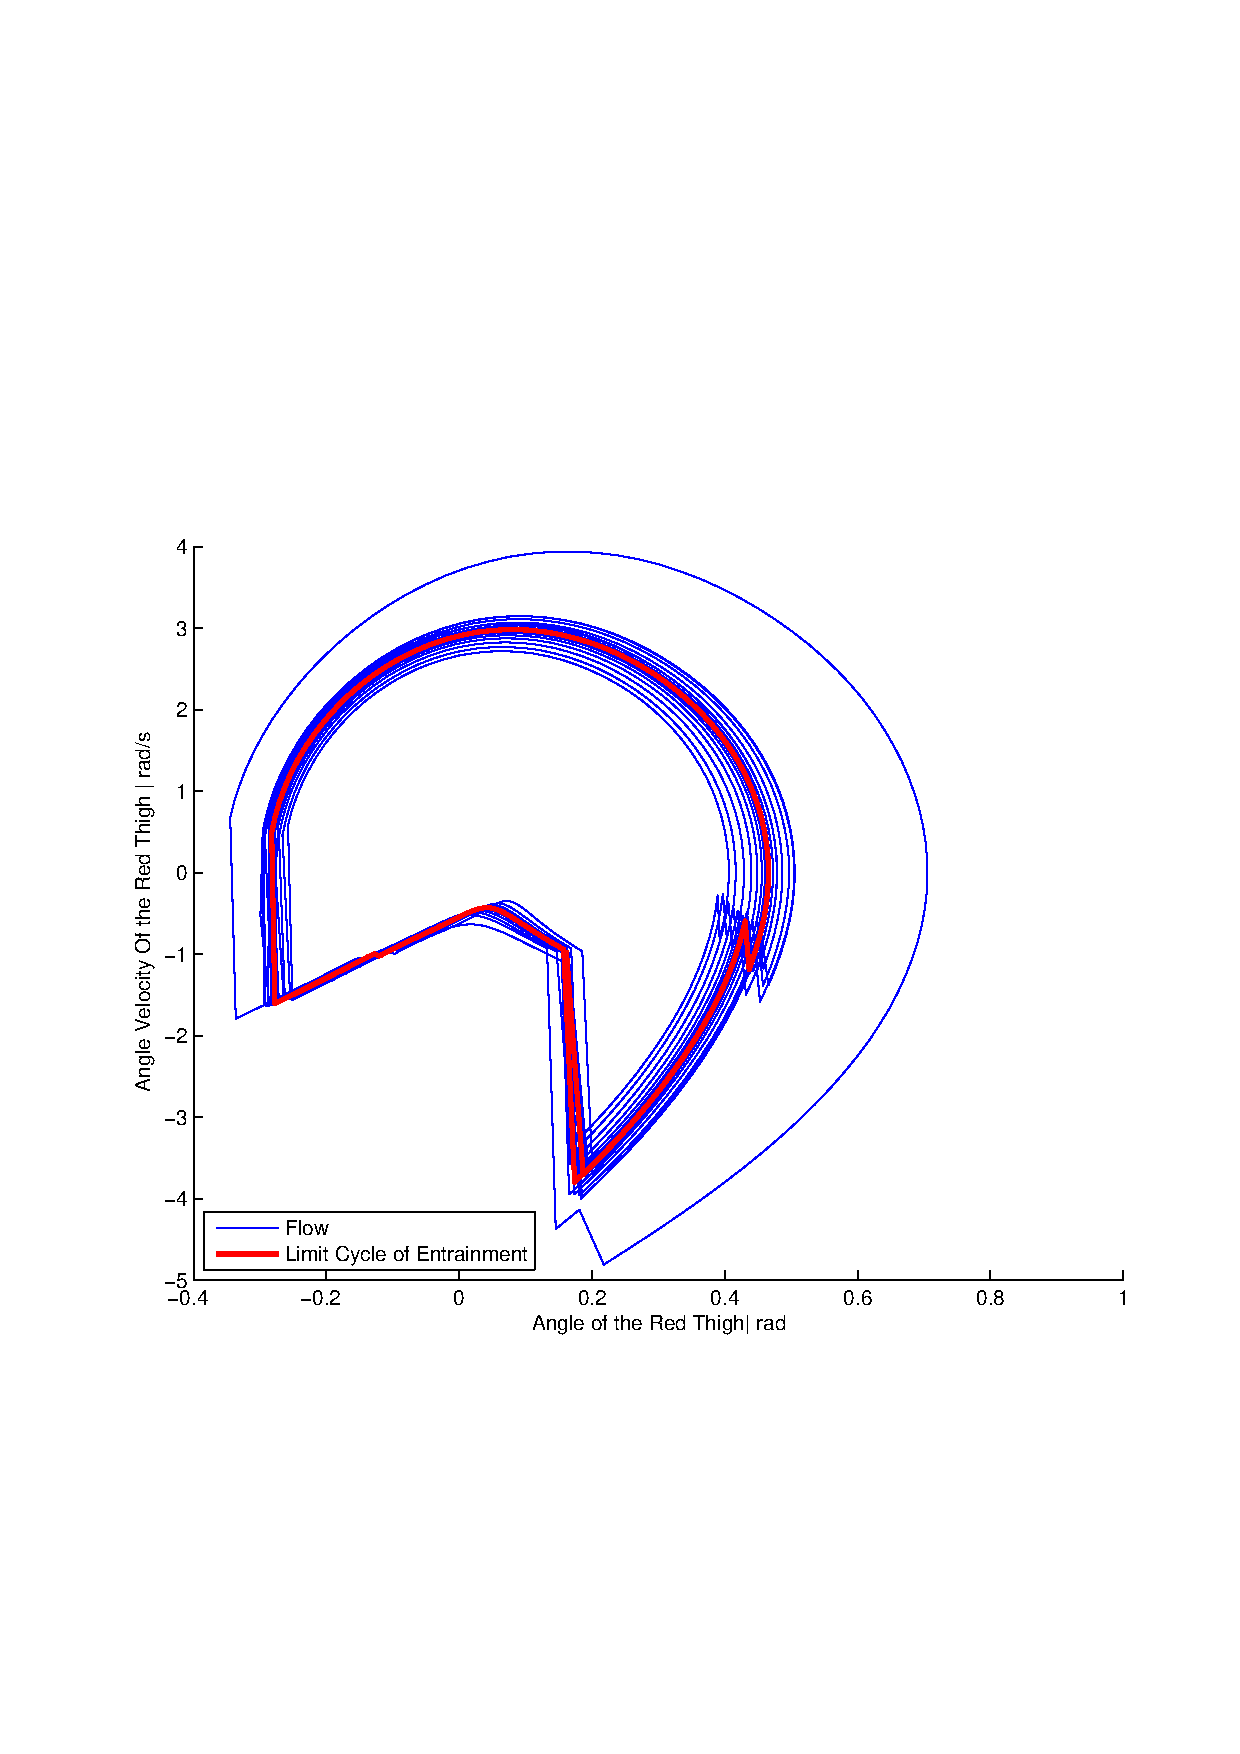
\includegraphics[width=0.7\textwidth]{PushWalkingPhasePlot}
    \caption{The Pushed Gait Phase Plot}
    \label{fig:PushGaitPlot}
\end{center}
\end{figure}


\begin{figure}[!htbp]
  \begin{center}
      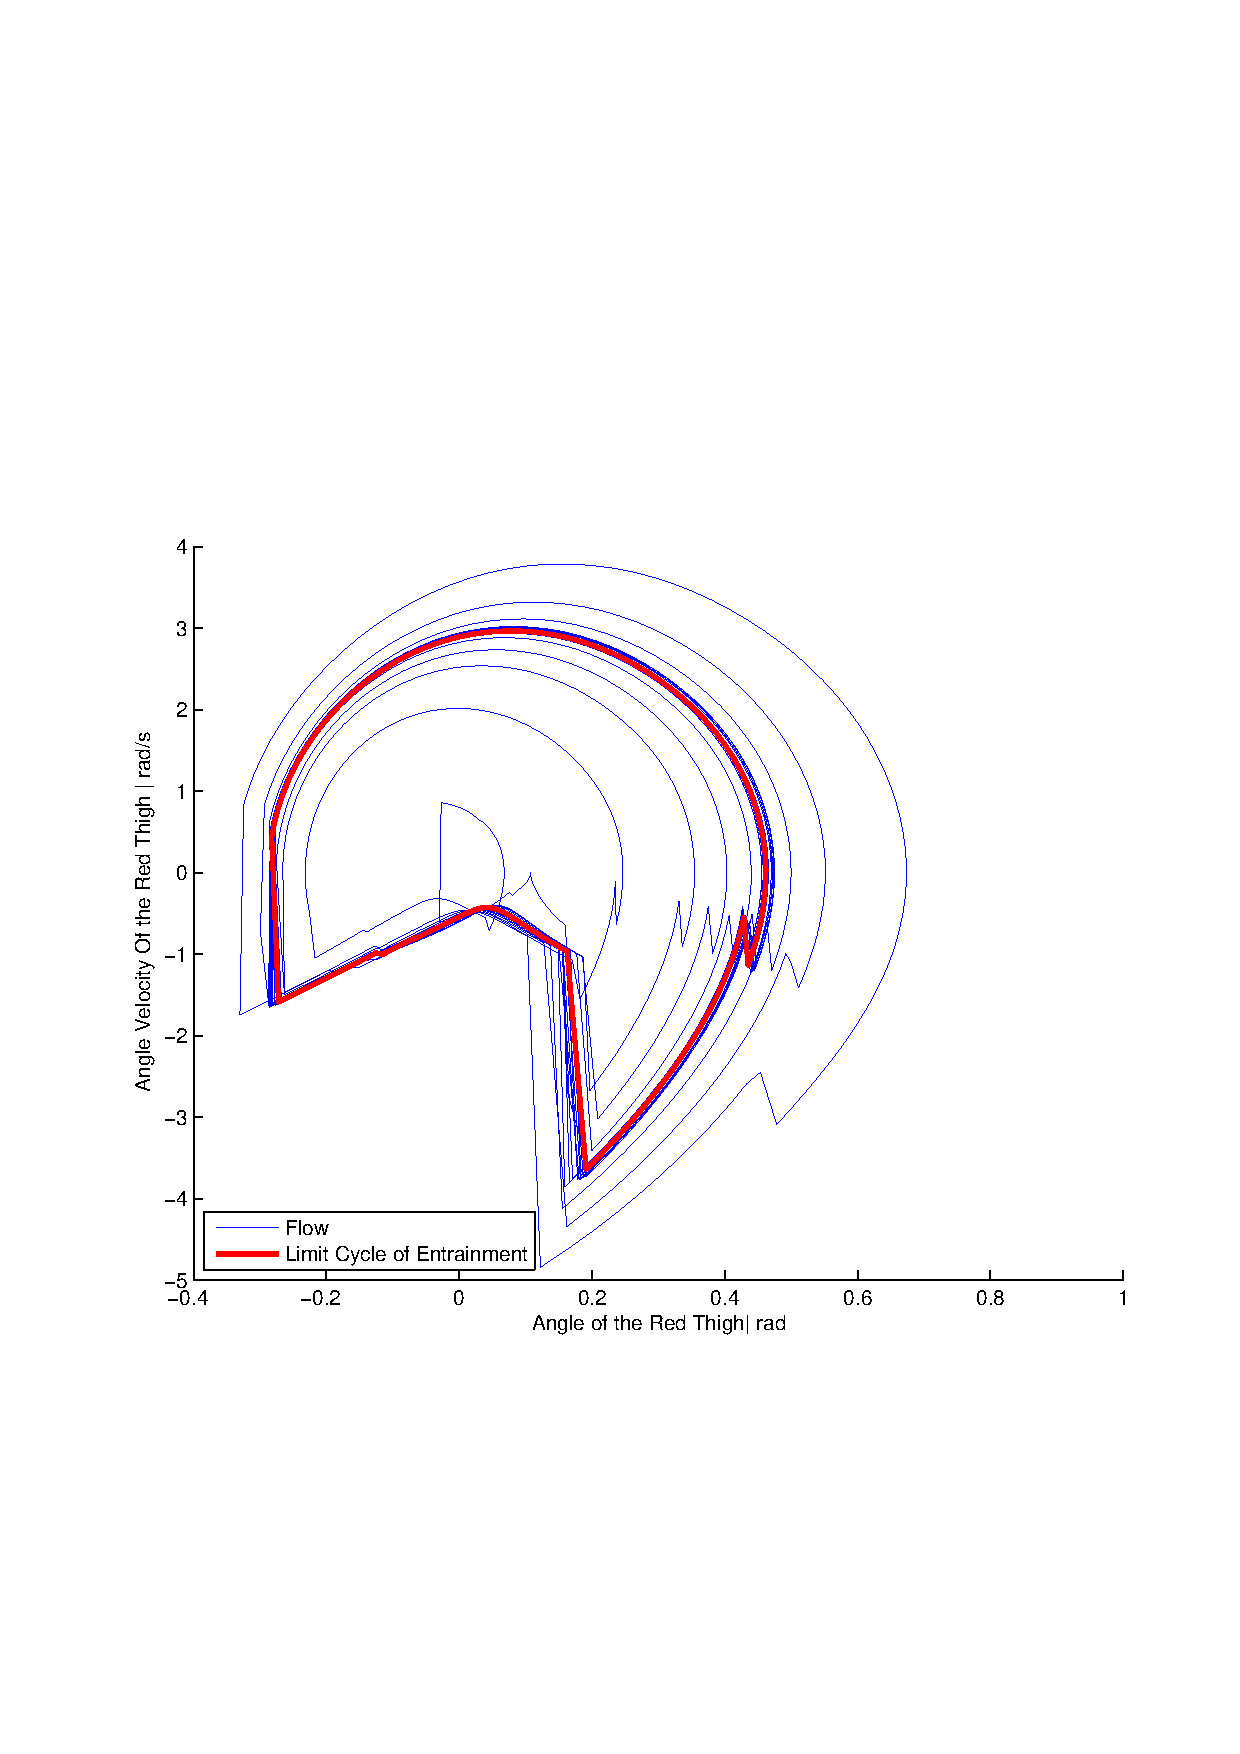
\includegraphics[width=0.7\textwidth]{PullWalkingPhasePlot}
    \caption{The Pulled Gait Phase Plot}
    \label{fig:PullGaitPhasePlot}
\end{center}
\end{figure}


Also the change the initial stepsize, the walker will adjust it automatically.
Figure~\ref{fig:bigStepIni} and Figure~\ref{fig:smallStepini} show the gaits.
Figure~\ref{fig:bigstepiniGaitPlot} and Figure~\ref{fig:smallstepiniPhasePlot} show the phase plot.

\begin{figure}[!htbp]
  \begin{center}
      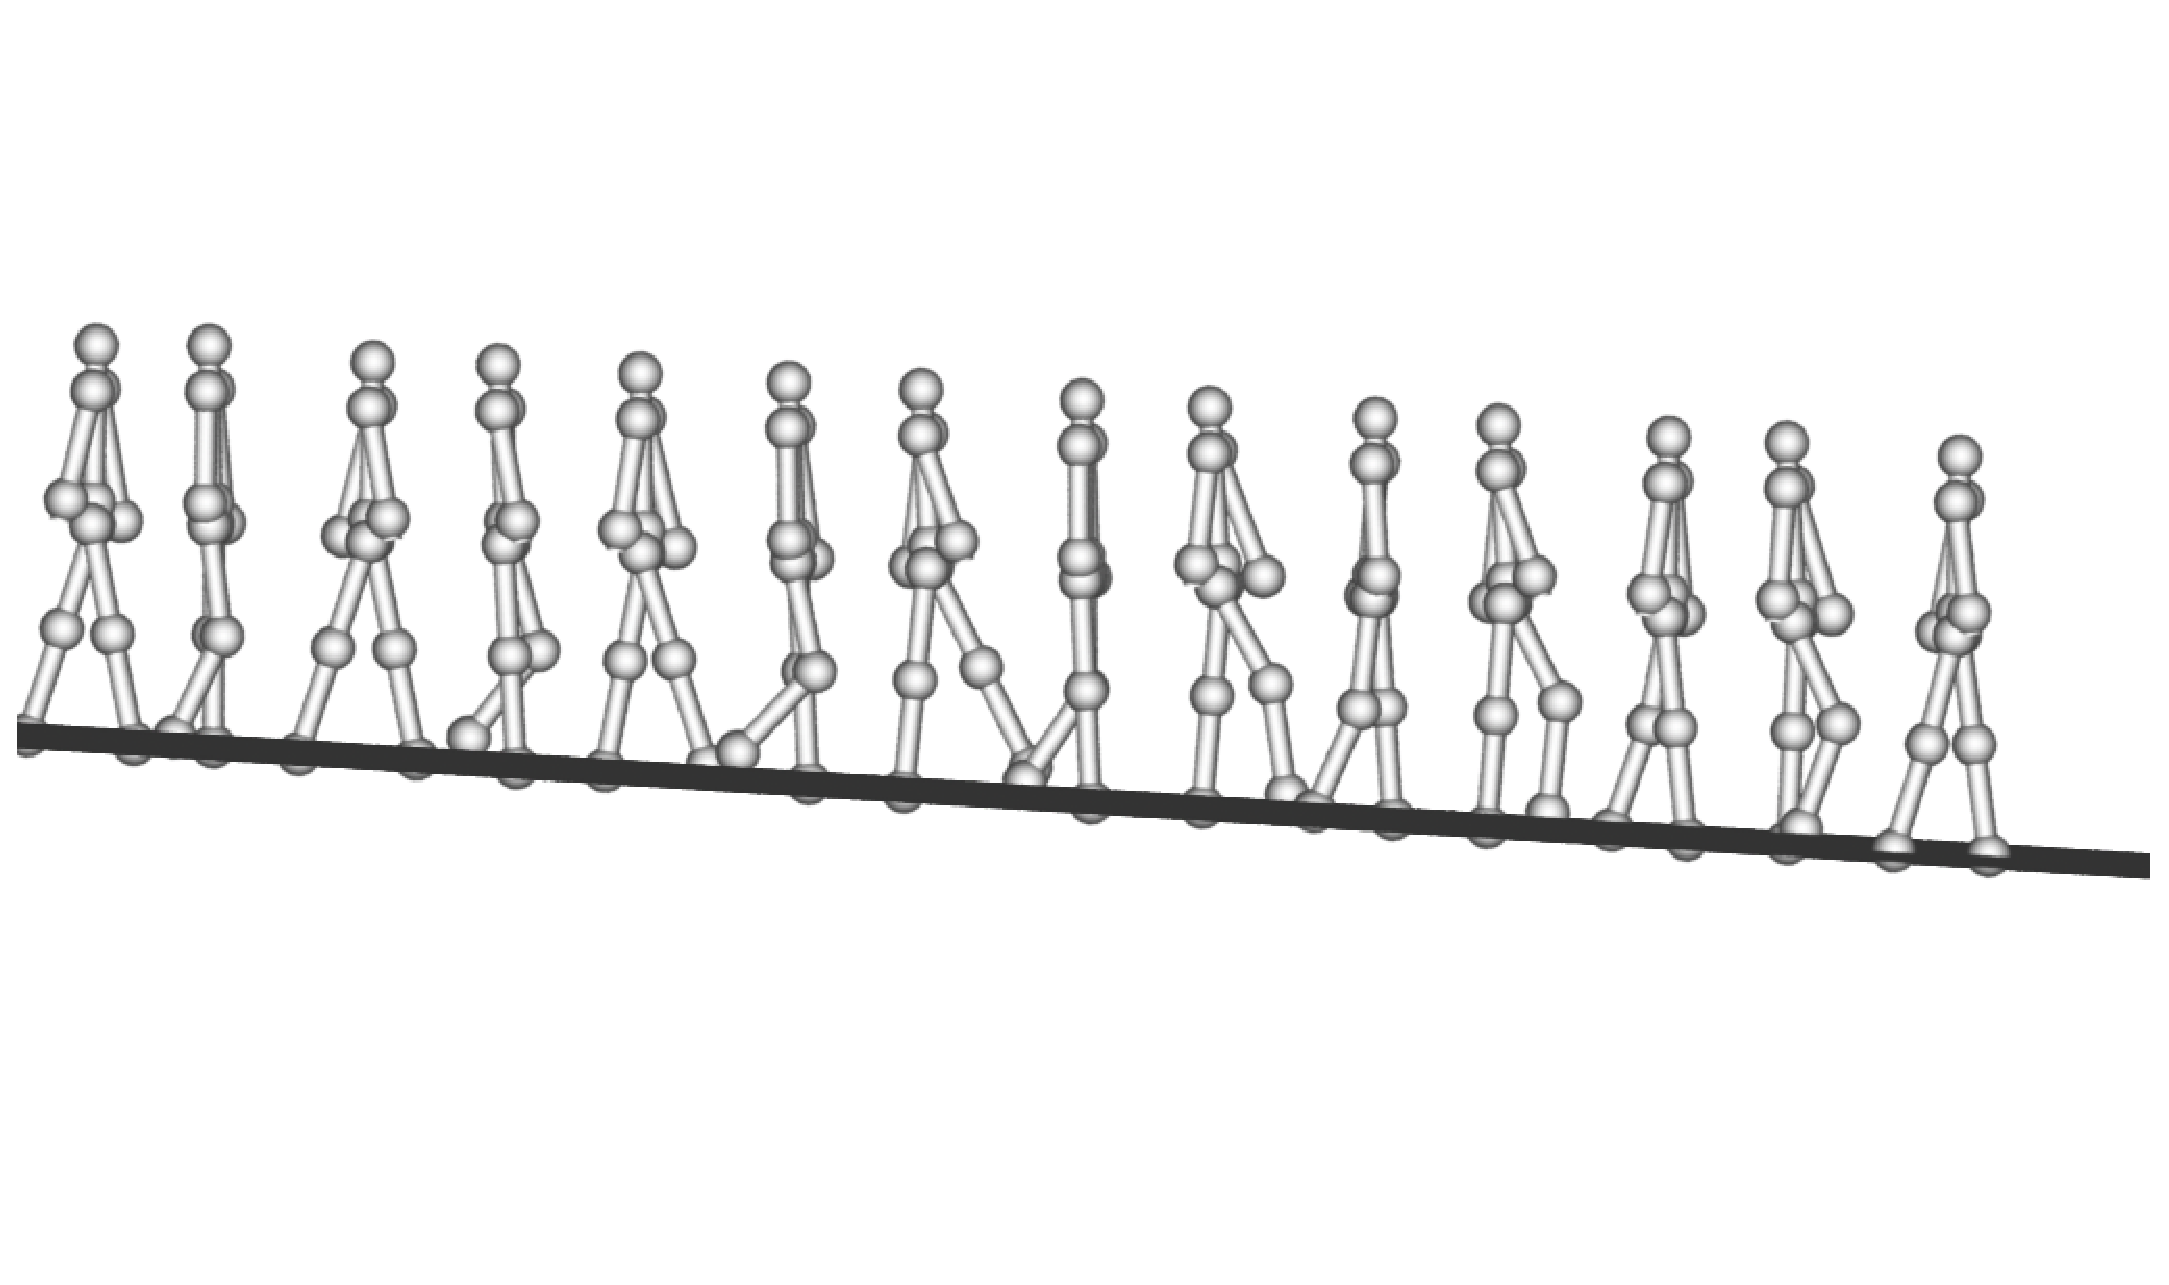
\includegraphics[width=0.7\textwidth]{BigStep}
    \caption{Big Initial Step Size}
    \label{fig:bigStepIni}
\end{center}
\end{figure}


\begin{figure}[!htbp]
  \begin{center}
      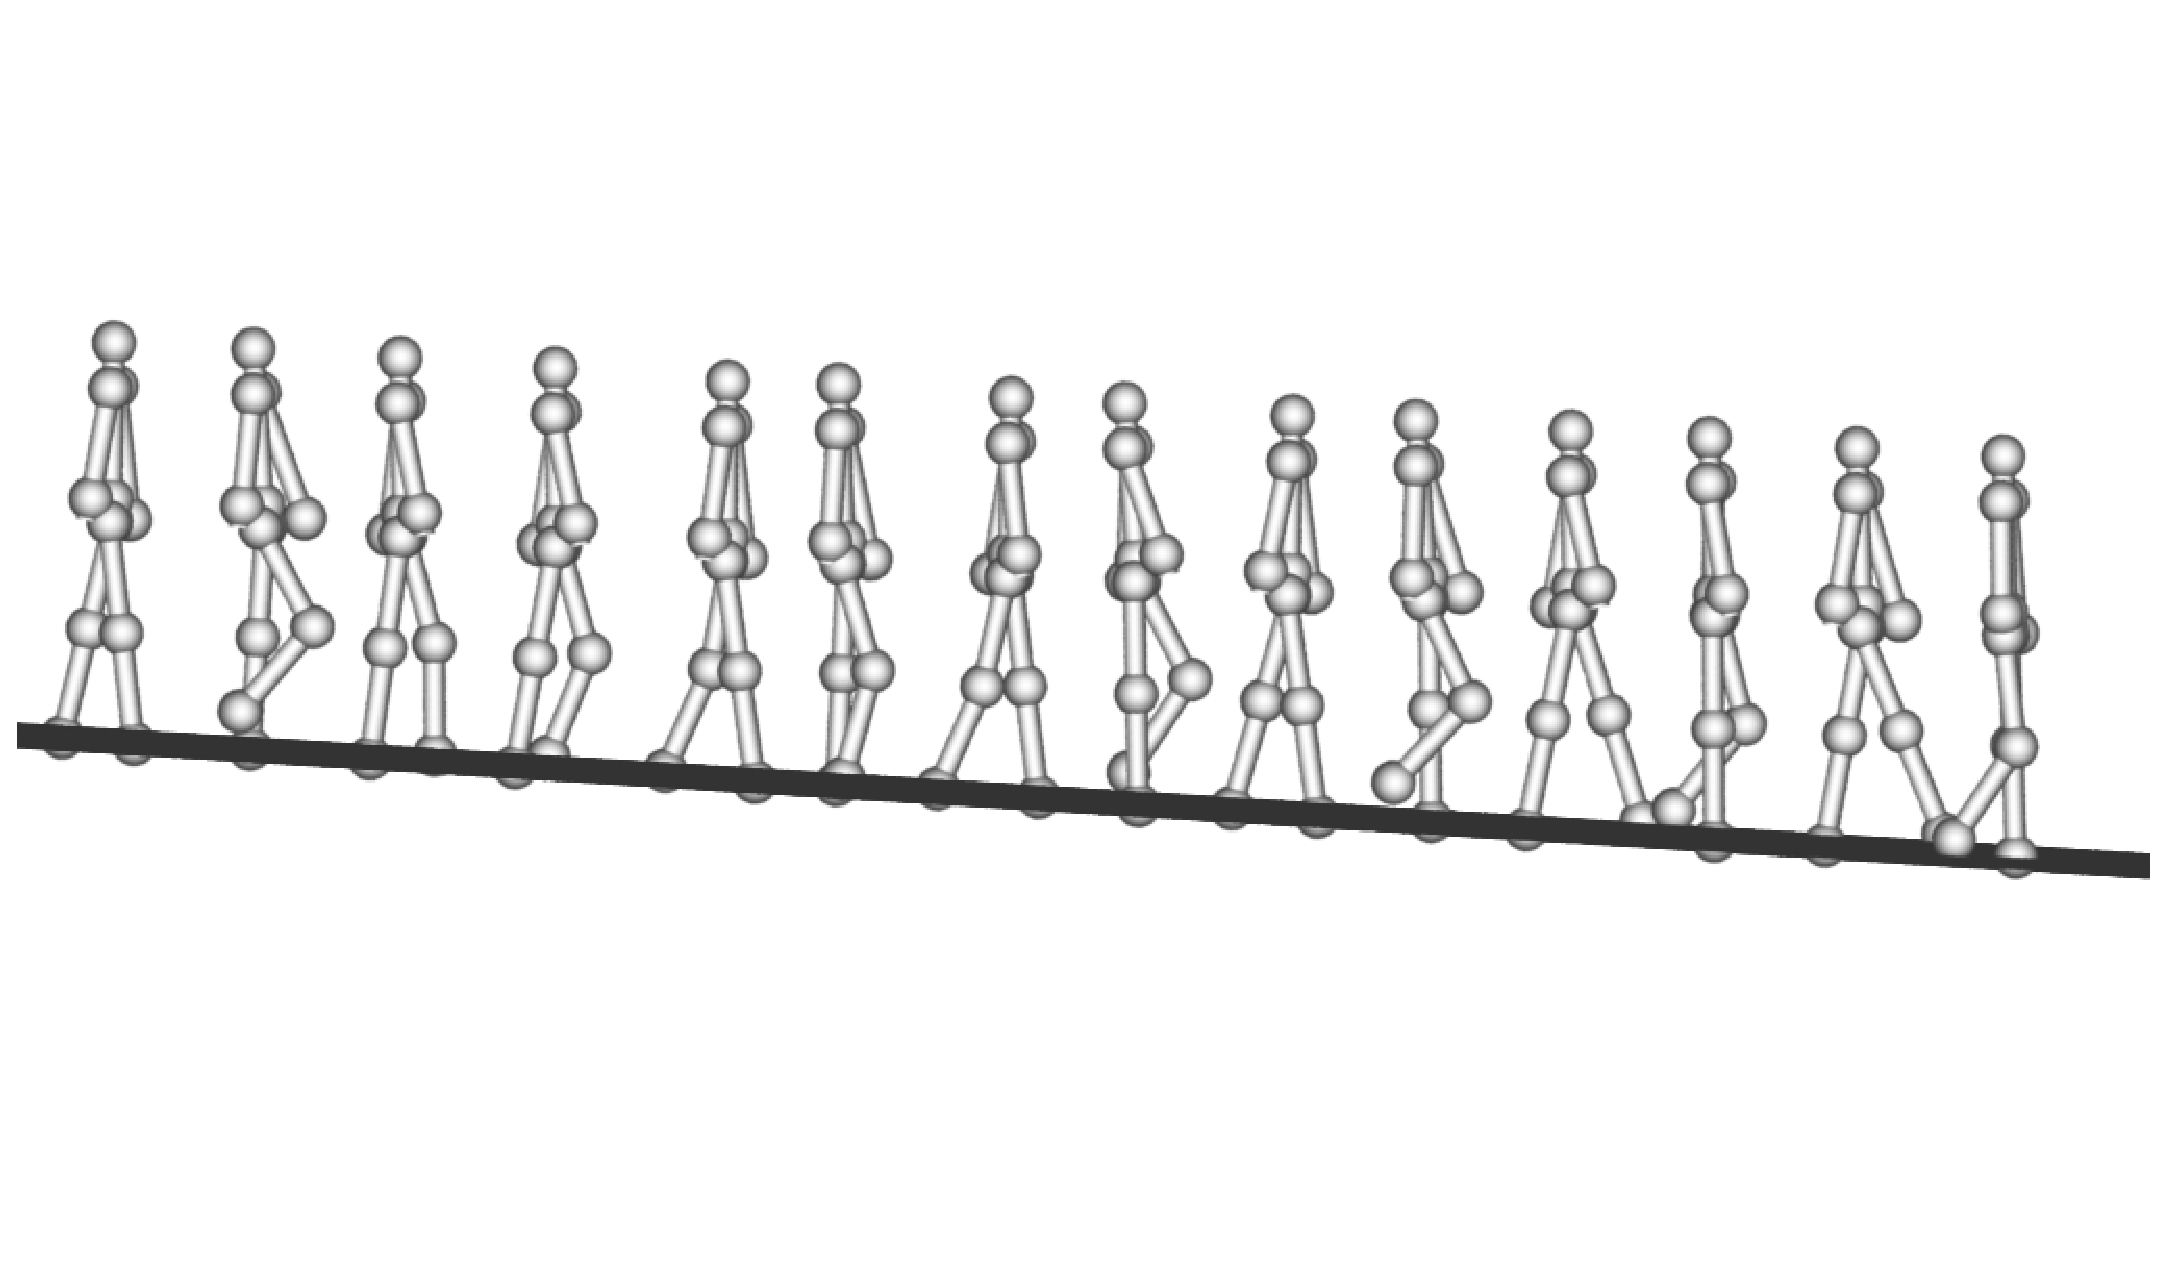
\includegraphics[width=0.7\textwidth]{smallStep}
    \caption{Small Initial Step Size}
    \label{fig:smallStepini}
\end{center}
\end{figure}


\begin{figure}[!htbp]
  \begin{center}
      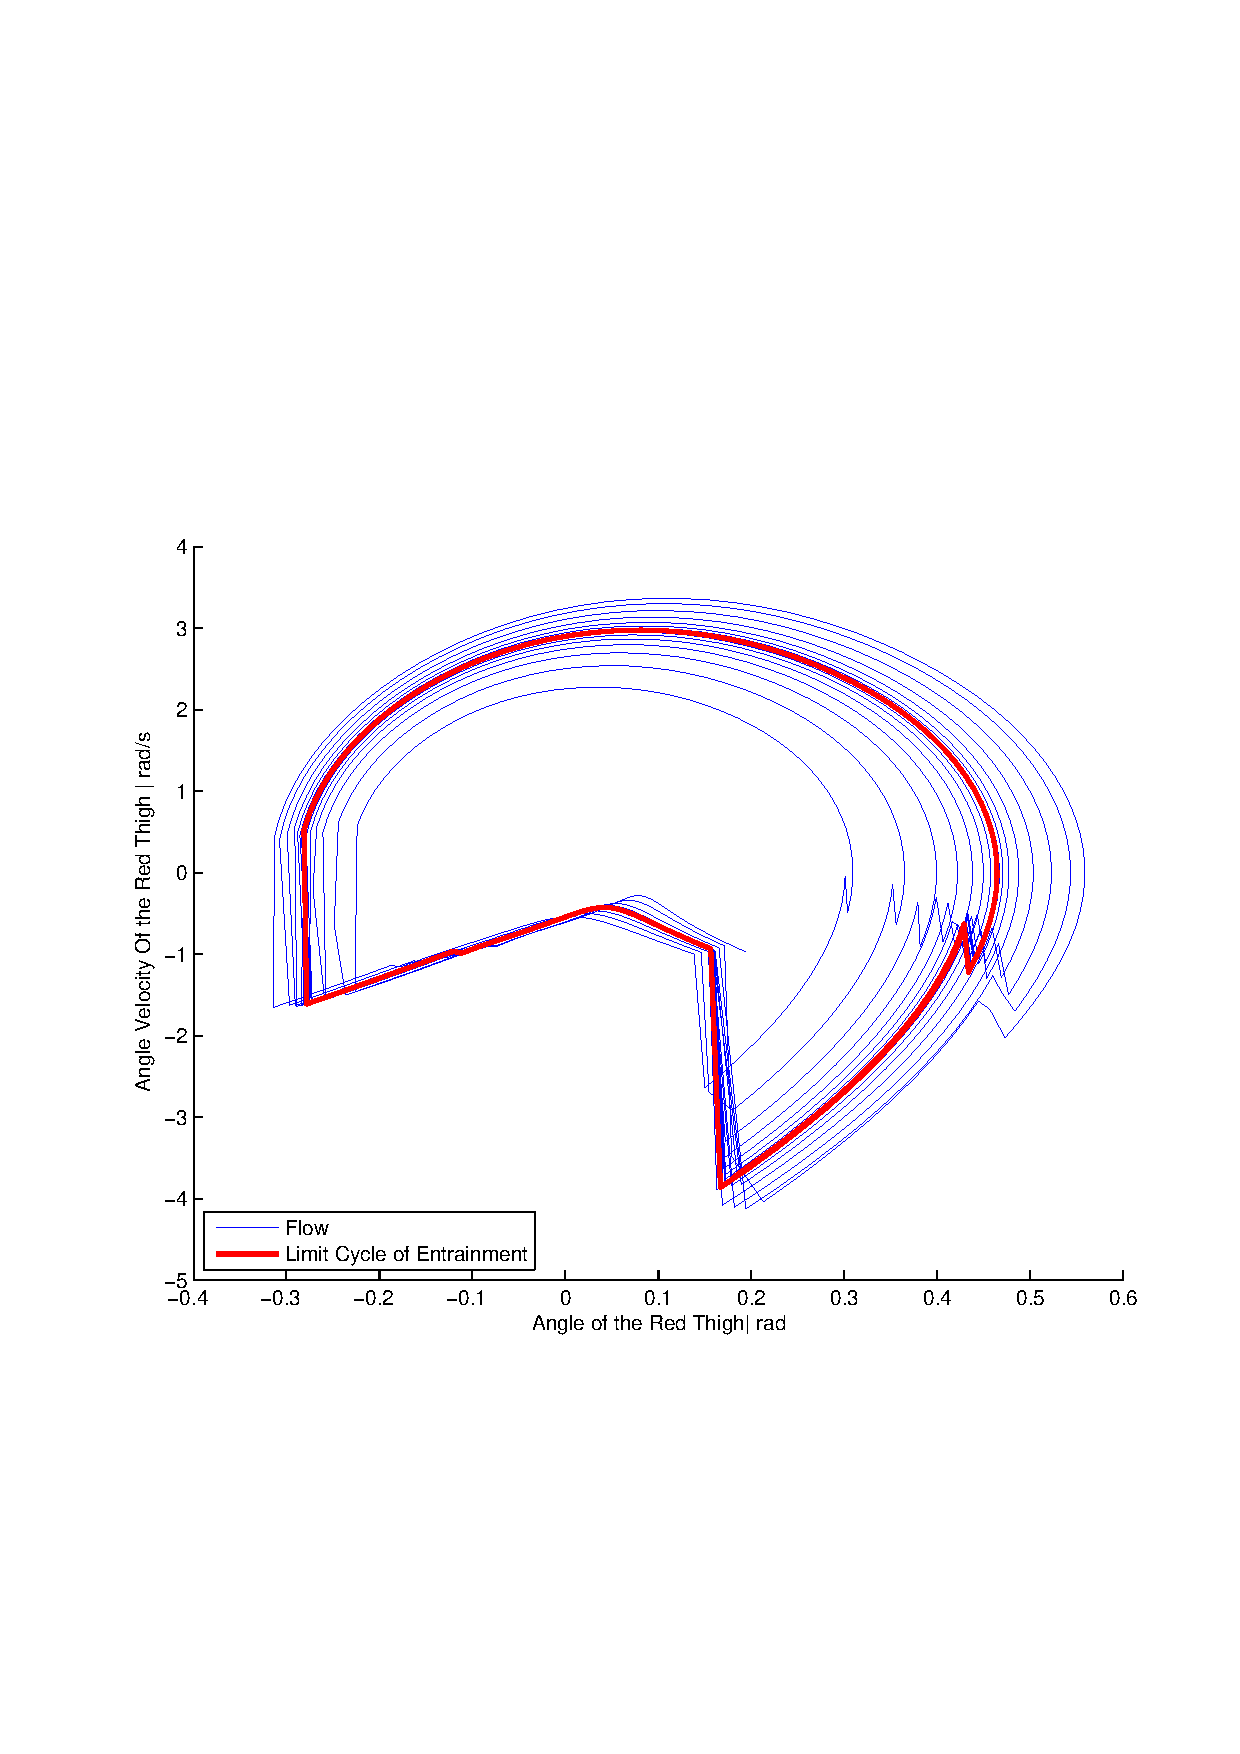
\includegraphics[width=0.7\textwidth]{BigStepPhasePlot}
    \caption{Big Initial Step Initial Phase Plot}
    \label{fig:bigstepiniGaitPlot}
\end{center}
\end{figure}


\begin{figure}[!htbp]
  \begin{center}
      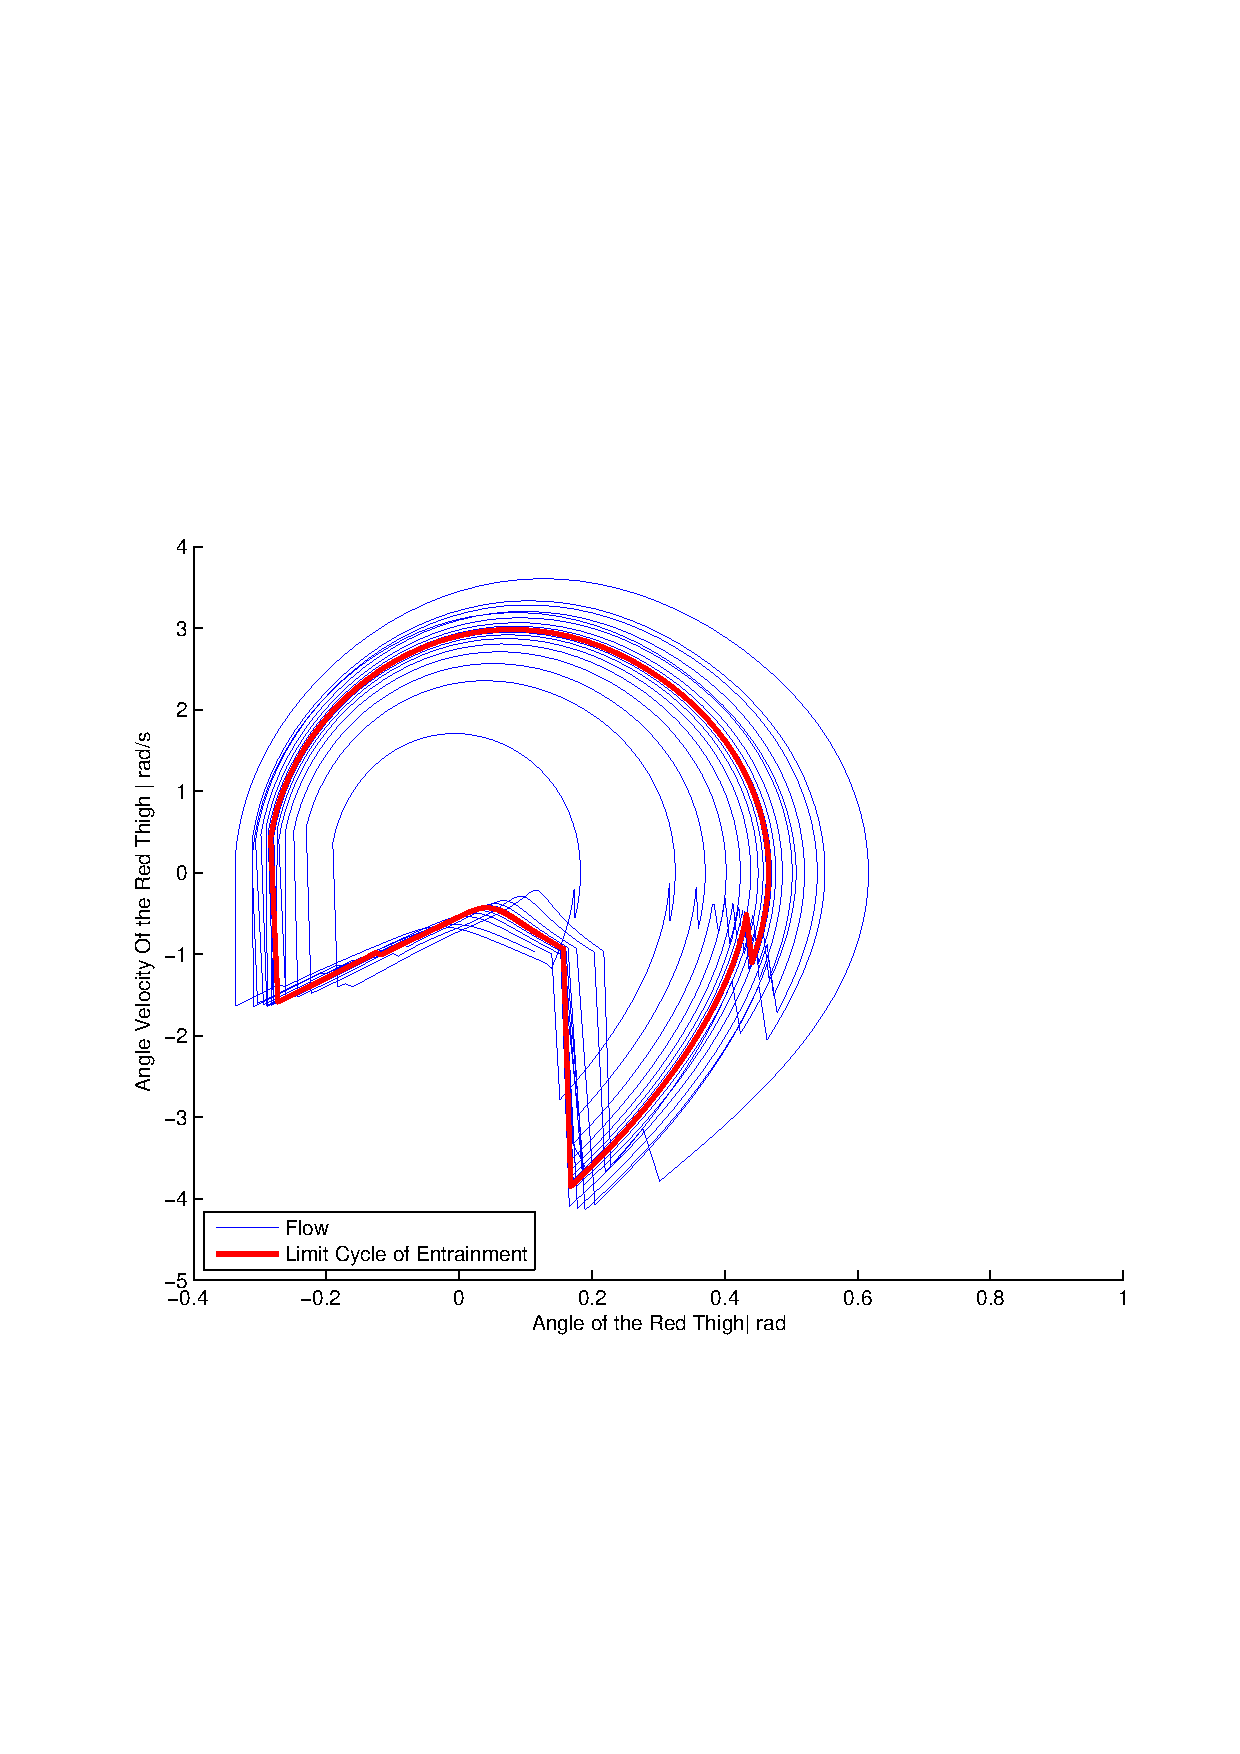
\includegraphics[width=0.7\textwidth]{SmallStepPhasePlot}
    \caption{The Small Initial Step Gait Phase Plot}
    \label{fig:smallstepiniPhasePlot}
\end{center}
\end{figure}







\subsection{System Gait Adaptation}
The passive dynamic system has many parameters, changing such parameters will generate different gait through system adaptation.
we can formulate the original system as
\[
\dot{\state}=F_a(\state)
\]
where $a$ is the system parameters.
we adjust the several parameters, neural oscillator maintain the limit cycle, but different parameters will generate different gait.
Some meaningful gait are shown.
Because uniform ally change the parameter will not effect the gaits, only will effect the period, so we most of the parameters we change is the ratio.
We will maintain the leg length $L$ and mass sum.
\subsubsection*{Mass Distribution Change}
We change the mass of the hip $m_h$, different $m_h$ will generate different gaits, while bigger $m_h$ will result motion that are similar to burdened gait.
different Limit Cycles are show in Figure ~\ref{fig_differentmh}
\begin{figure}[!htbp]
  \begin{center}
      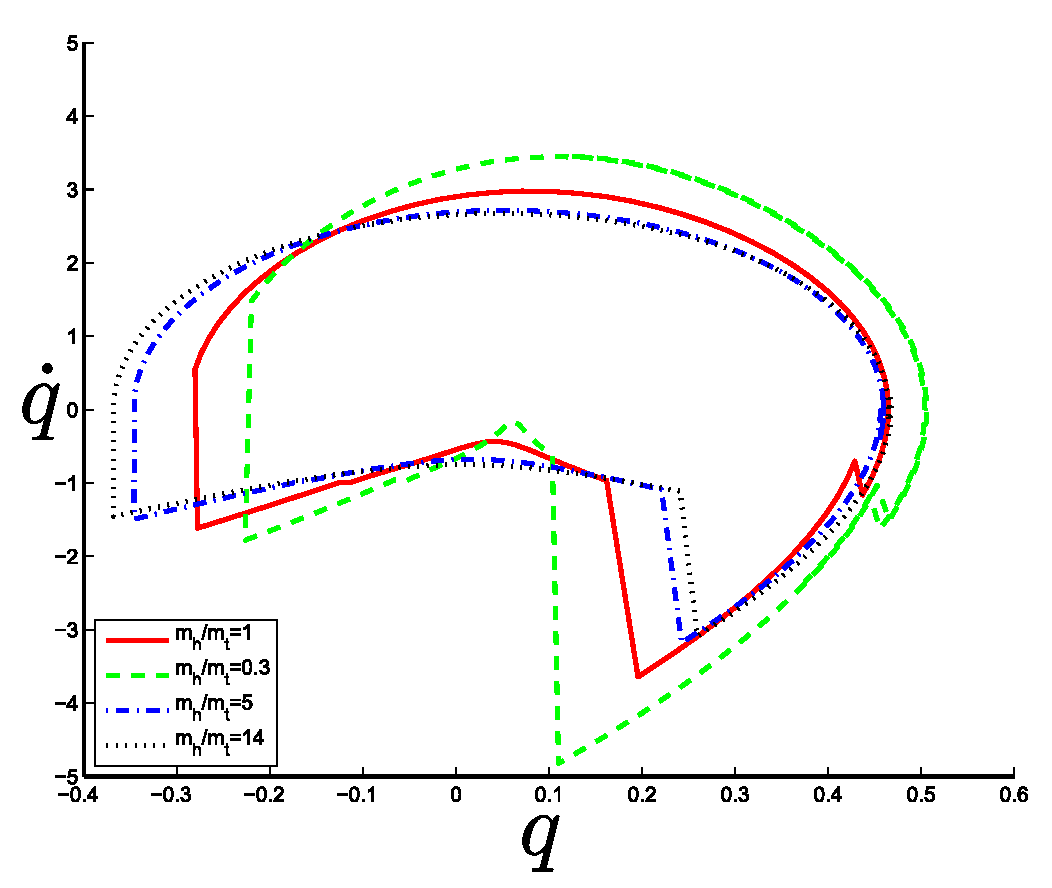
\includegraphics[width=0.7\textwidth]{MassDistributionEffectsOnLimitCircle}
    \caption{Different Gait Resulting From the Different Mass Ratio}
    \label{fig:differentmh}
\end{center}
\end{figure}

From the phase plot, we find some interesting tendency,
when the hip is heavier, it will walk with bigger step but a slow speed($\qd$ is lower),and also character tend to fall backward.
which the body is become litter, character will walk with quickly($\qd$ is bigger) and it tends to lean forward.

This may give us some information about the upper body motion.
Usually, when we carry something heavier, we  tend to bend the body upper forward to prevent following backward.

different gaits are show in the following pictures.
\begin{figure}[!htbp]
  \begin{center}
      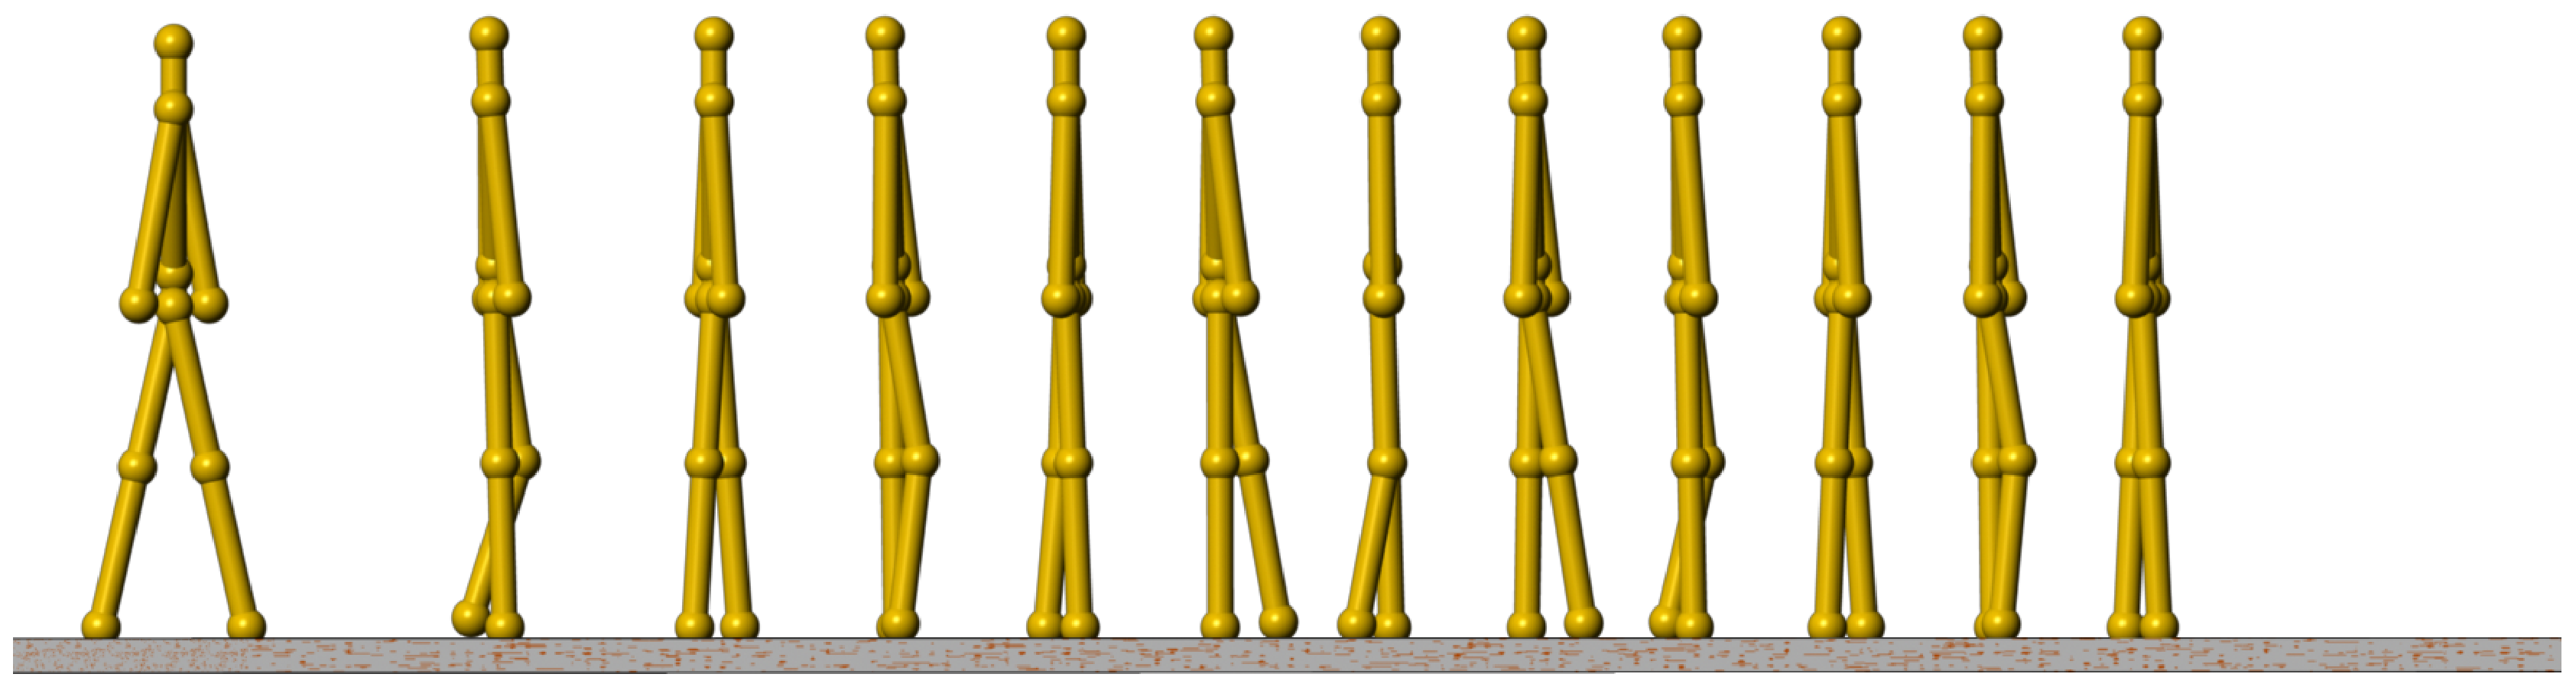
\includegraphics[width=0.7\textwidth]{walking_with_neural}
    \caption{Place Holder}
    \label{fig:massh1}
\end{center}
\end{figure}

\begin{figure}[!htbp]
  \begin{center}
      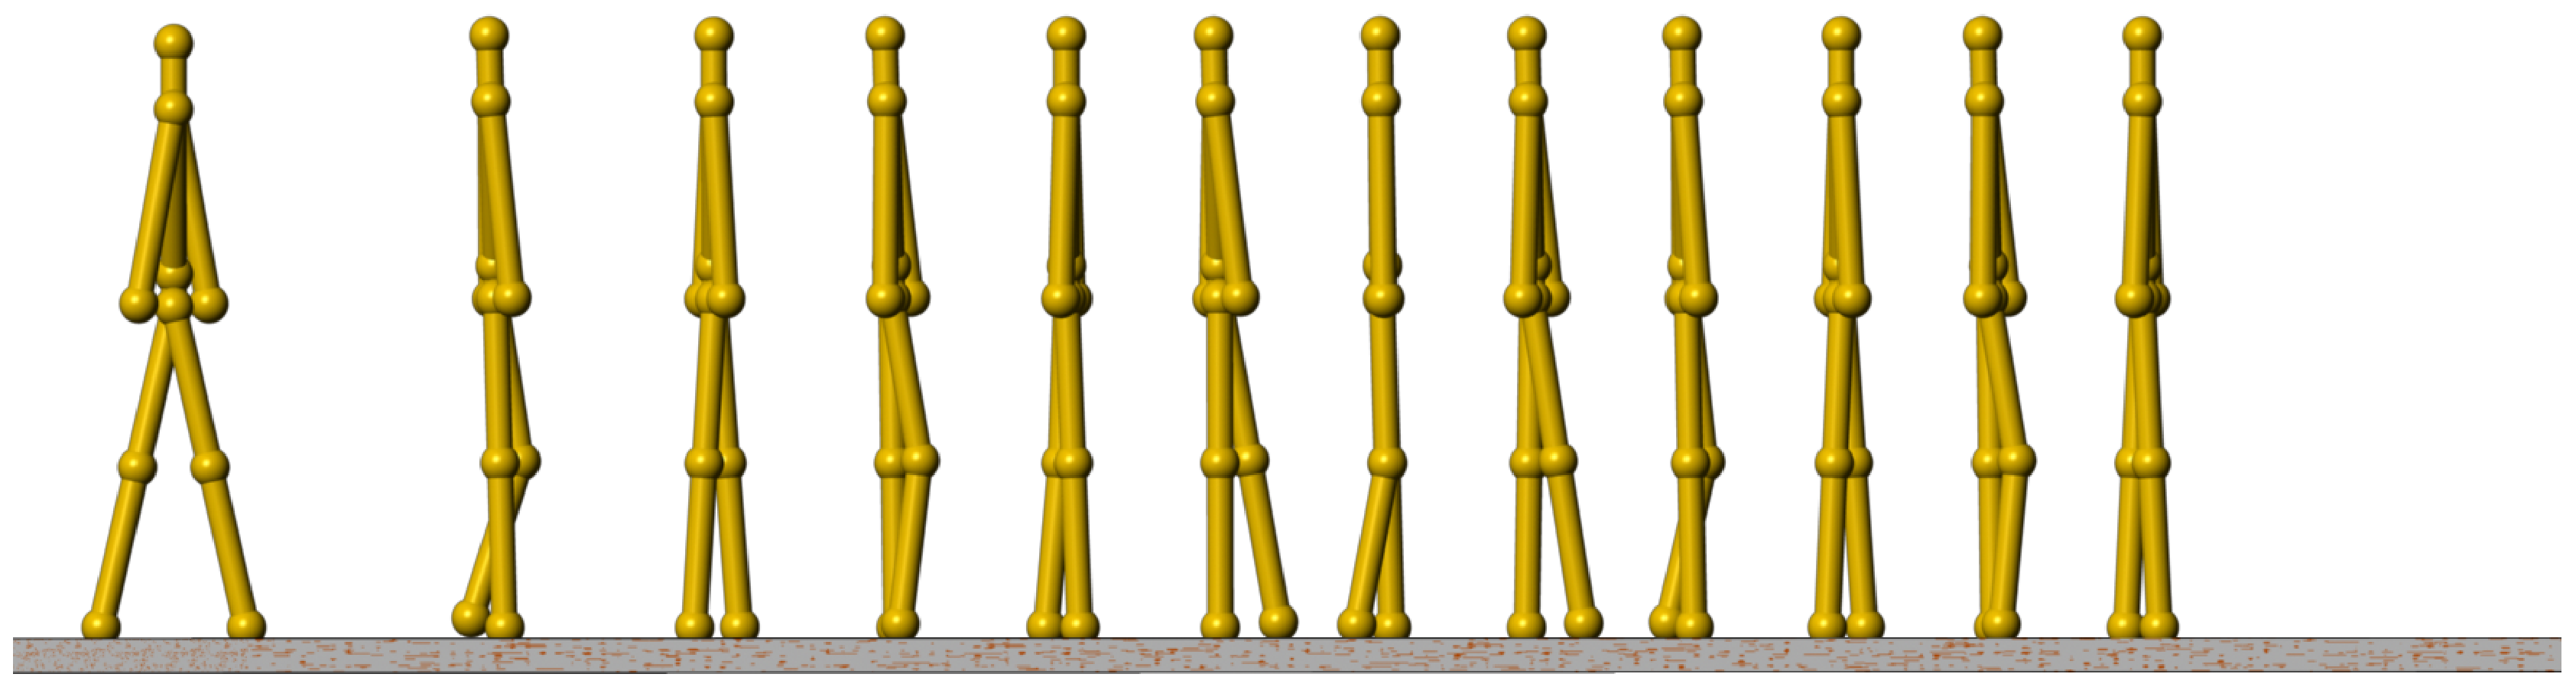
\includegraphics[width=0.7\textwidth]{walking_with_neural}
    \caption{Place Holder}
    \label{fig:massh2}
\end{center}
\end{figure}

\begin{figure}[!htbp]
  \begin{center}
      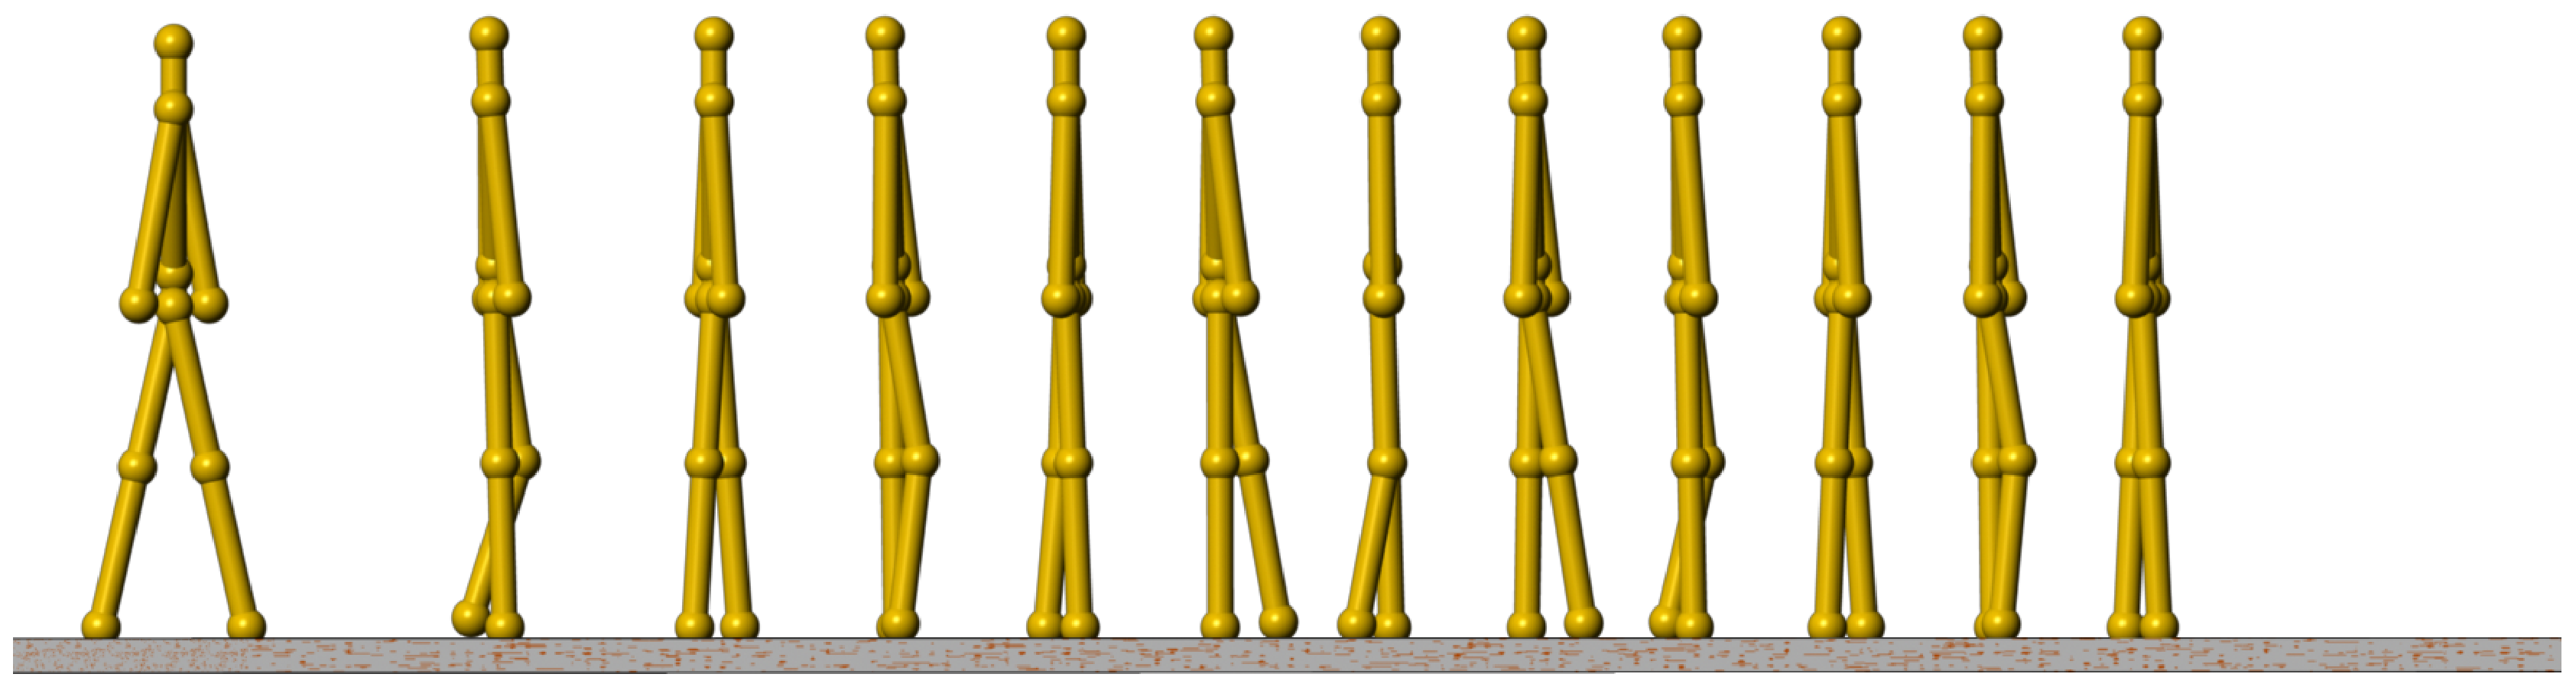
\includegraphics[width=0.7\textwidth]{walking_with_neural}
    \caption{Place Holder}
    \label{fig:massh3}
\end{center}
\end{figure}

%Mh/Mt=0.3

%Mh/Mt=2

%Mh/Mt=3

	
%Mh/mt=10


\subsubsection*{Leg Length Distribution Change}
we keep the leg length unchanged, but alter the ration of shank and thigh.
We generate gait with different leg length ratio.
as shown in figure~\ref{fig:differentlr}

\begin{figure}[!htbp]
  \begin{center}
    \leavevmode
    \ifpdf
      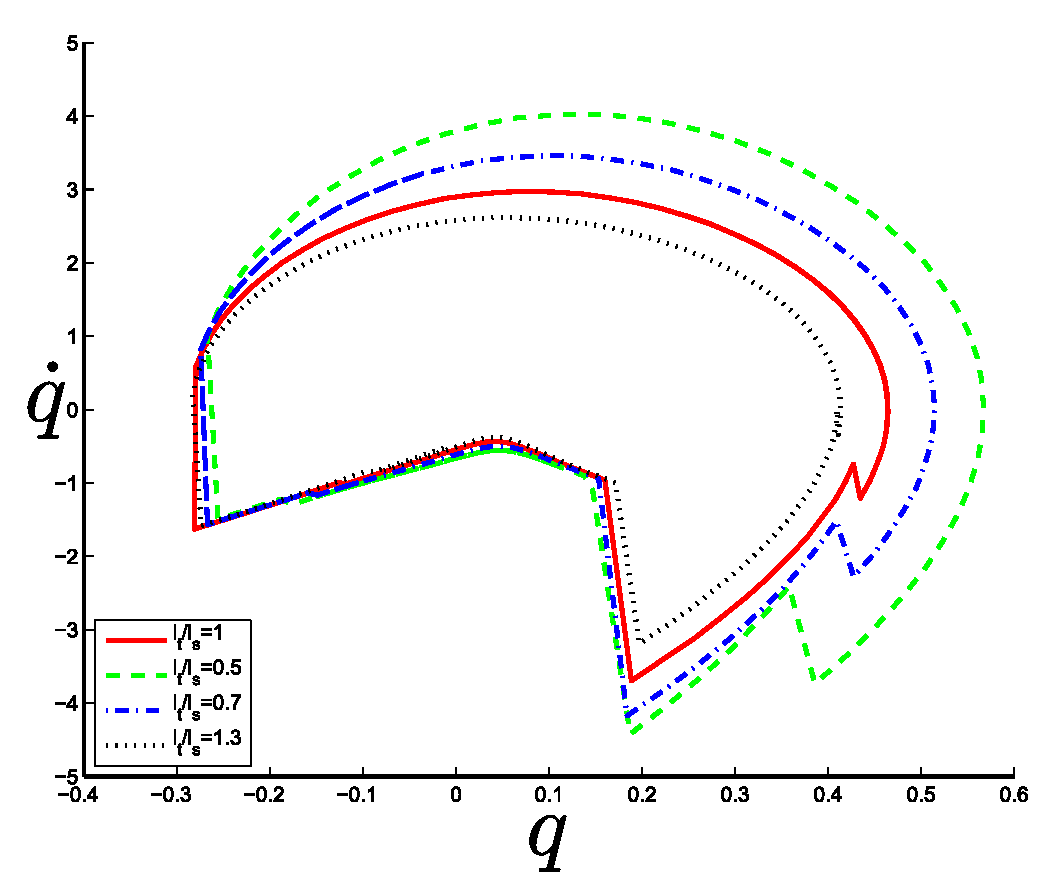
\includegraphics[height=6in]{LegLengthDistributionEffectsOnLimitCircle}
    \else
      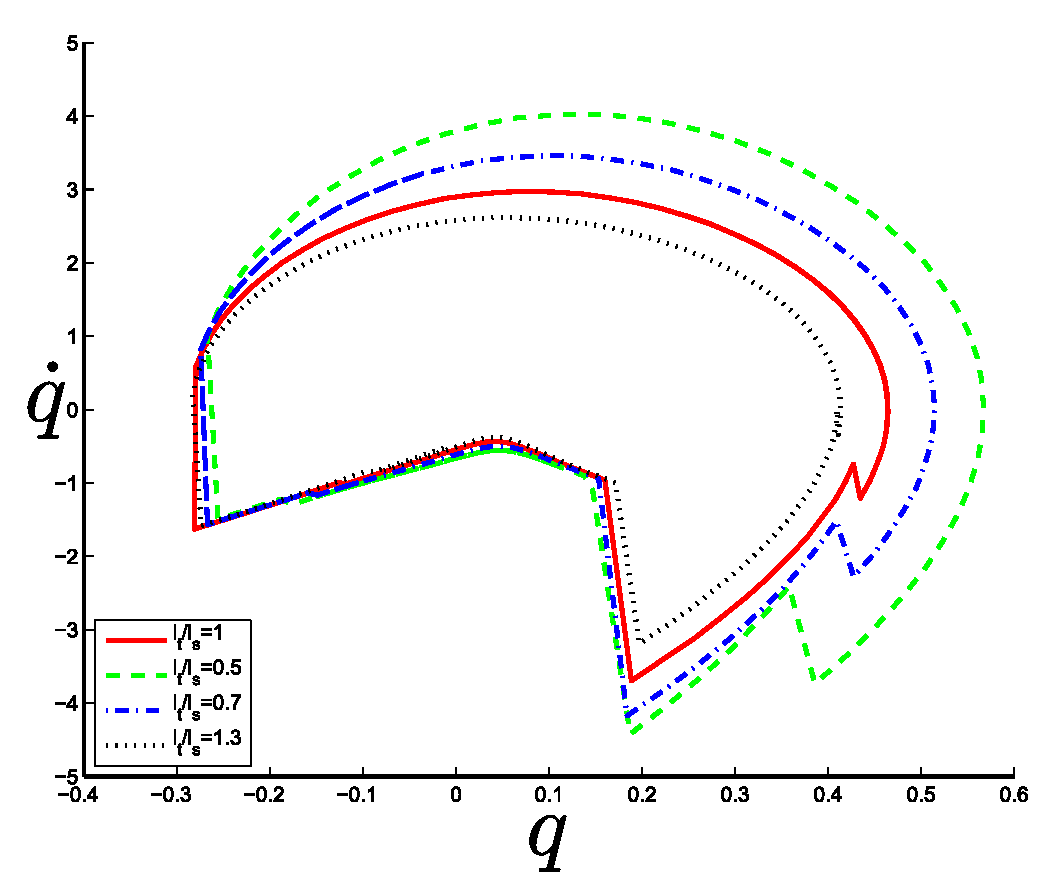
\includegraphics[width=0.7\textwidth]{LegLengthDistributionEffectsOnLimitCircle}
    \fi
    \caption{Different Gait Resulting From the Different Mass Ratio}
    \label{fig:differentlr}
\end{center}
\end{figure}

for the limit cycle in figure~\ref{fig:differentlr}, we find something interesting.
Basically, the support leg motion is almost the same, while different leg length ration will result in different sway angle
Basically the longer the shank, thigh has to sway quickly and with bigger amplitude.
There are also bigger impulses during the strike phase. For both the knee and heel strike, larger impulse is generated.
while step size is kept.
This maybe true that girls walking with tall heel will easily get knees and heel injured and also will generate larger step sound.


\begin{figure}[!htbp]
  \begin{center}
      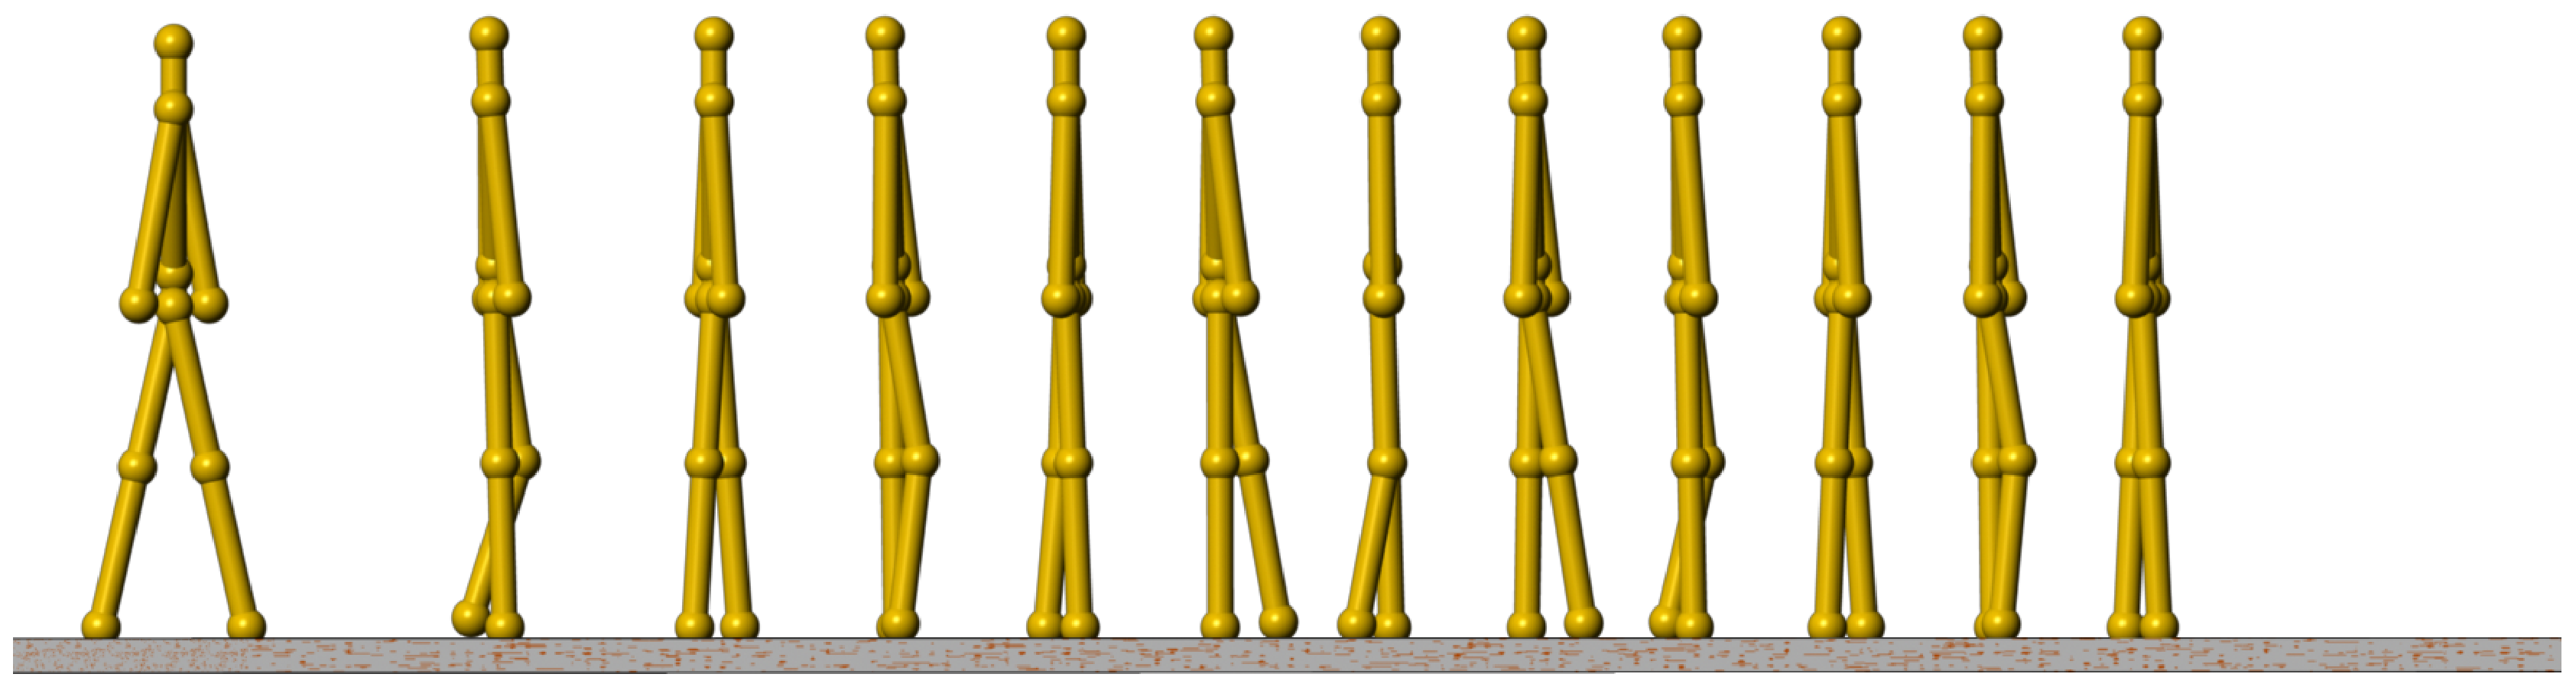
\includegraphics[width=0.7\textwidth]{walking_with_neural}
    \caption{Place Holder1}
    \label{fig:lr1}
\end{center}
\end{figure}

\begin{figure}[!htbp]
  \begin{center}
      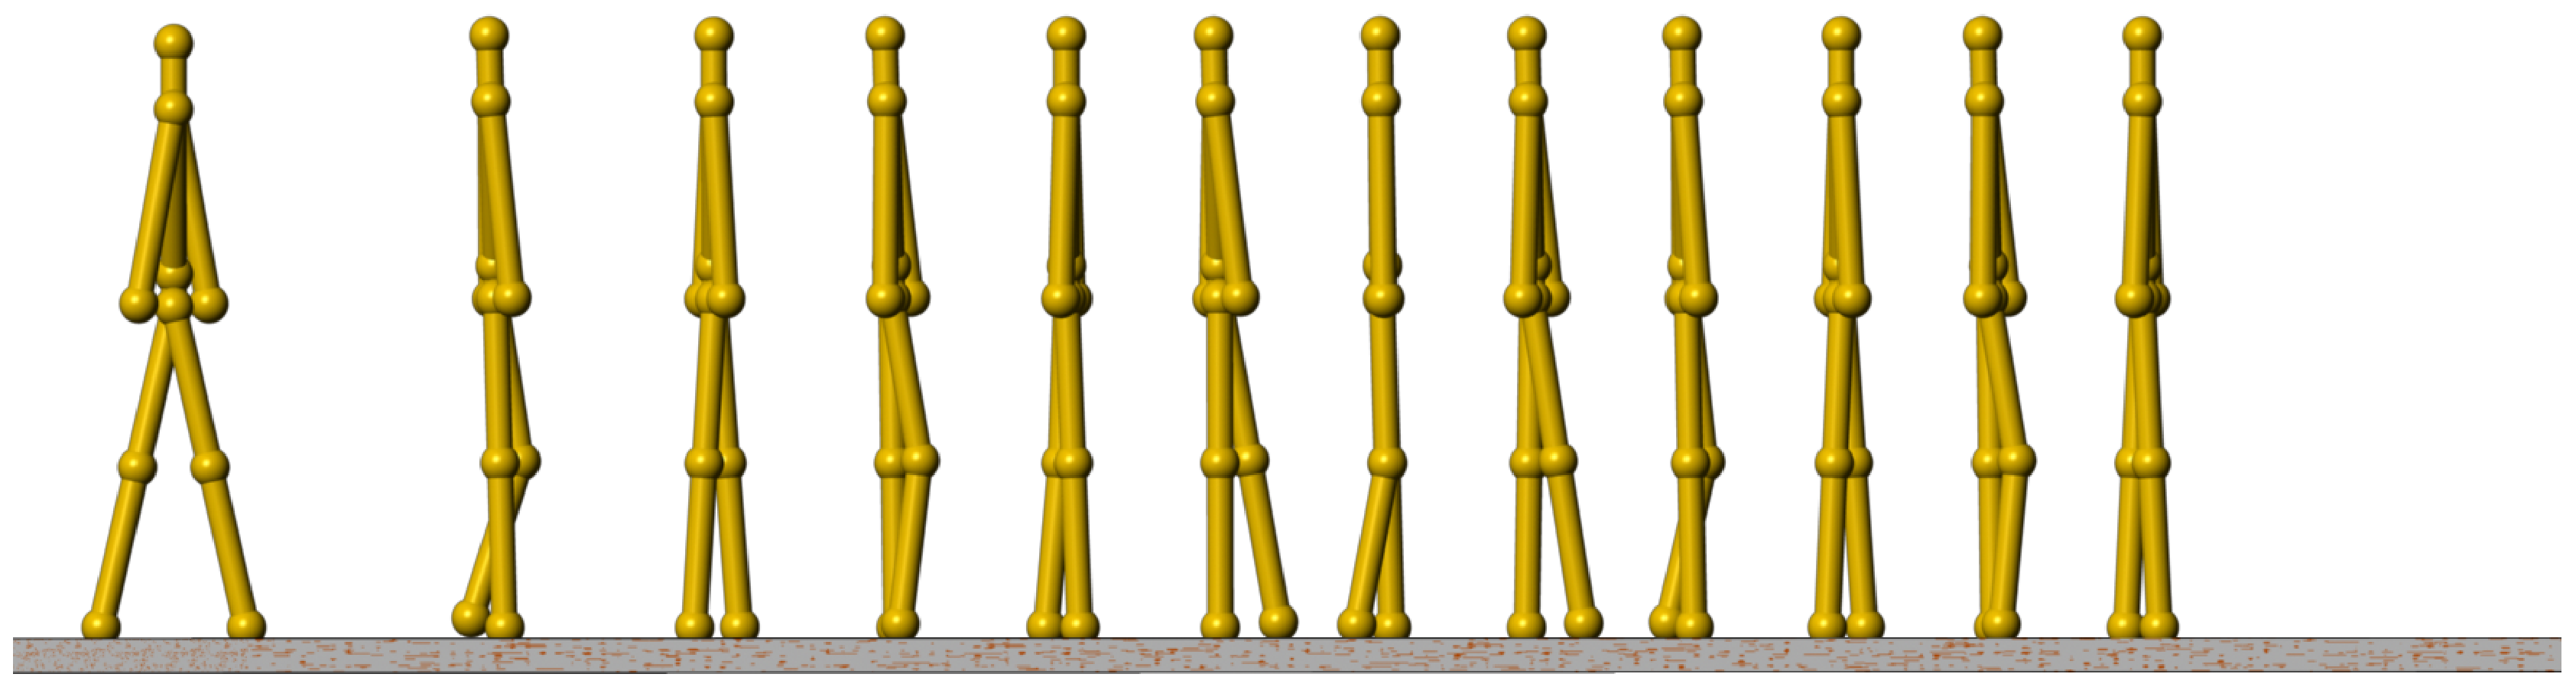
\includegraphics[width=0.7\textwidth]{walking_with_neural}
    \caption{Place Holder2}
    \label{fig:lr2}
\end{center}
\end{figure}

\begin{figure}[!htbp]
  \begin{center}
      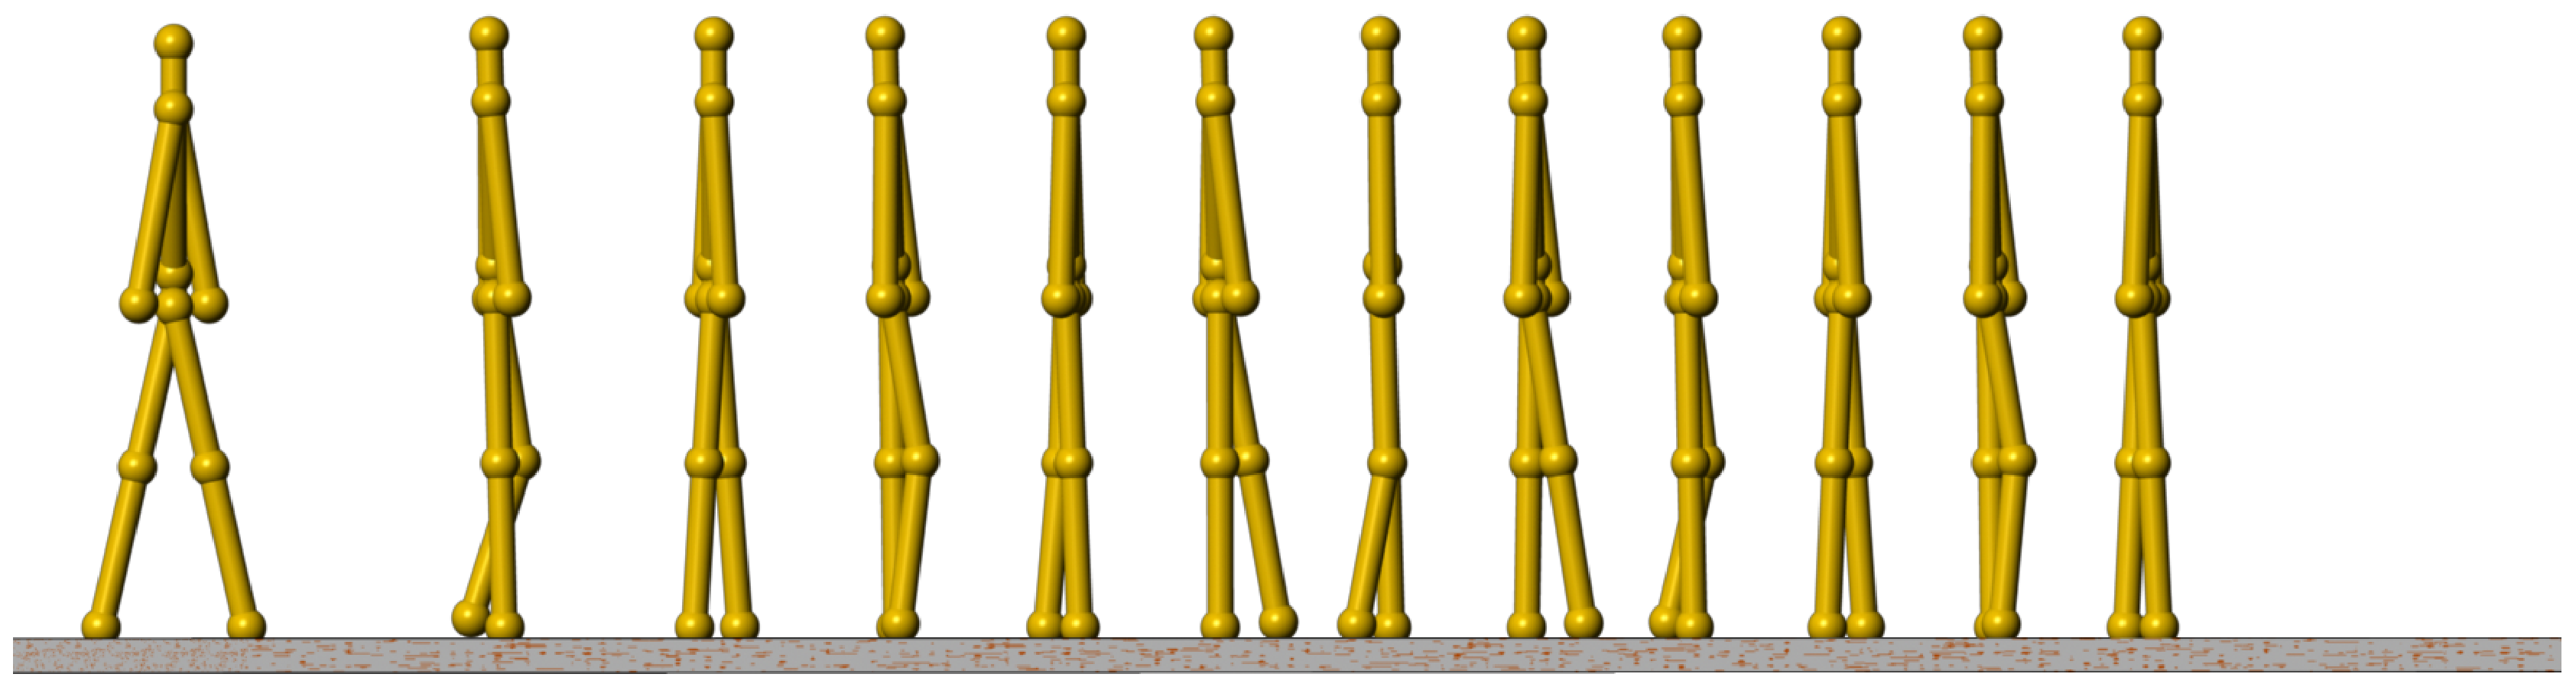
\includegraphics[width=0.7\textwidth]{walking_with_neural}
    \caption{Place Holder3}
    \label{fig:lr3}
\end{center}
\end{figure}




\subsubsection*{SlopChange}
Also we can change different down slope.
For different slope, entrainment maintained the limit cycle, but limit cycle changed its shape.
different stable limit circles are show in figure ~\ref{fig:diffstepsize}
Basically, the bigger the slope, the bigger the step size the higher the speed, and produce a gait similar to energy scaling.

\begin{figure}[!htbp]
  \begin{center}
    \leavevmode
    \ifpdf
      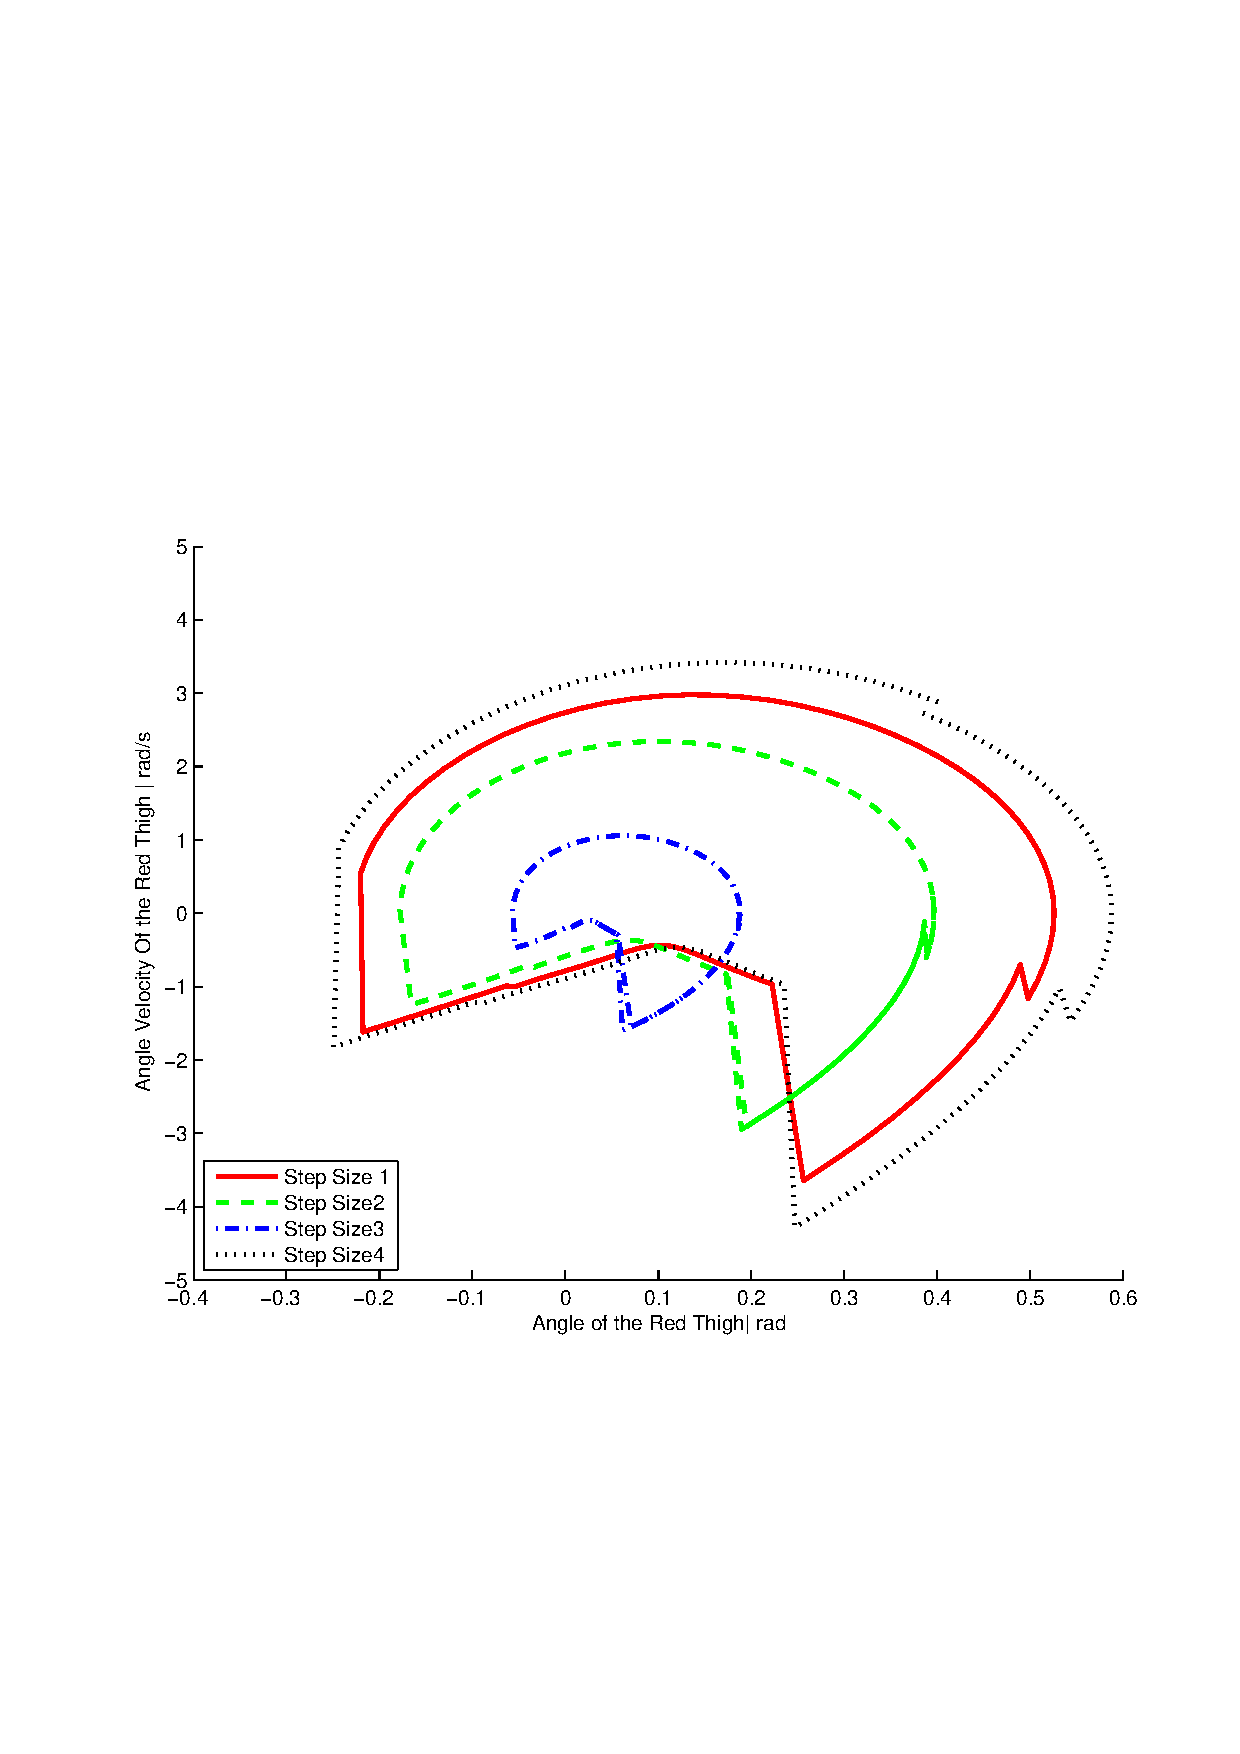
\includegraphics[height=6in]{DifferentStepSizeWalking}
    \else
      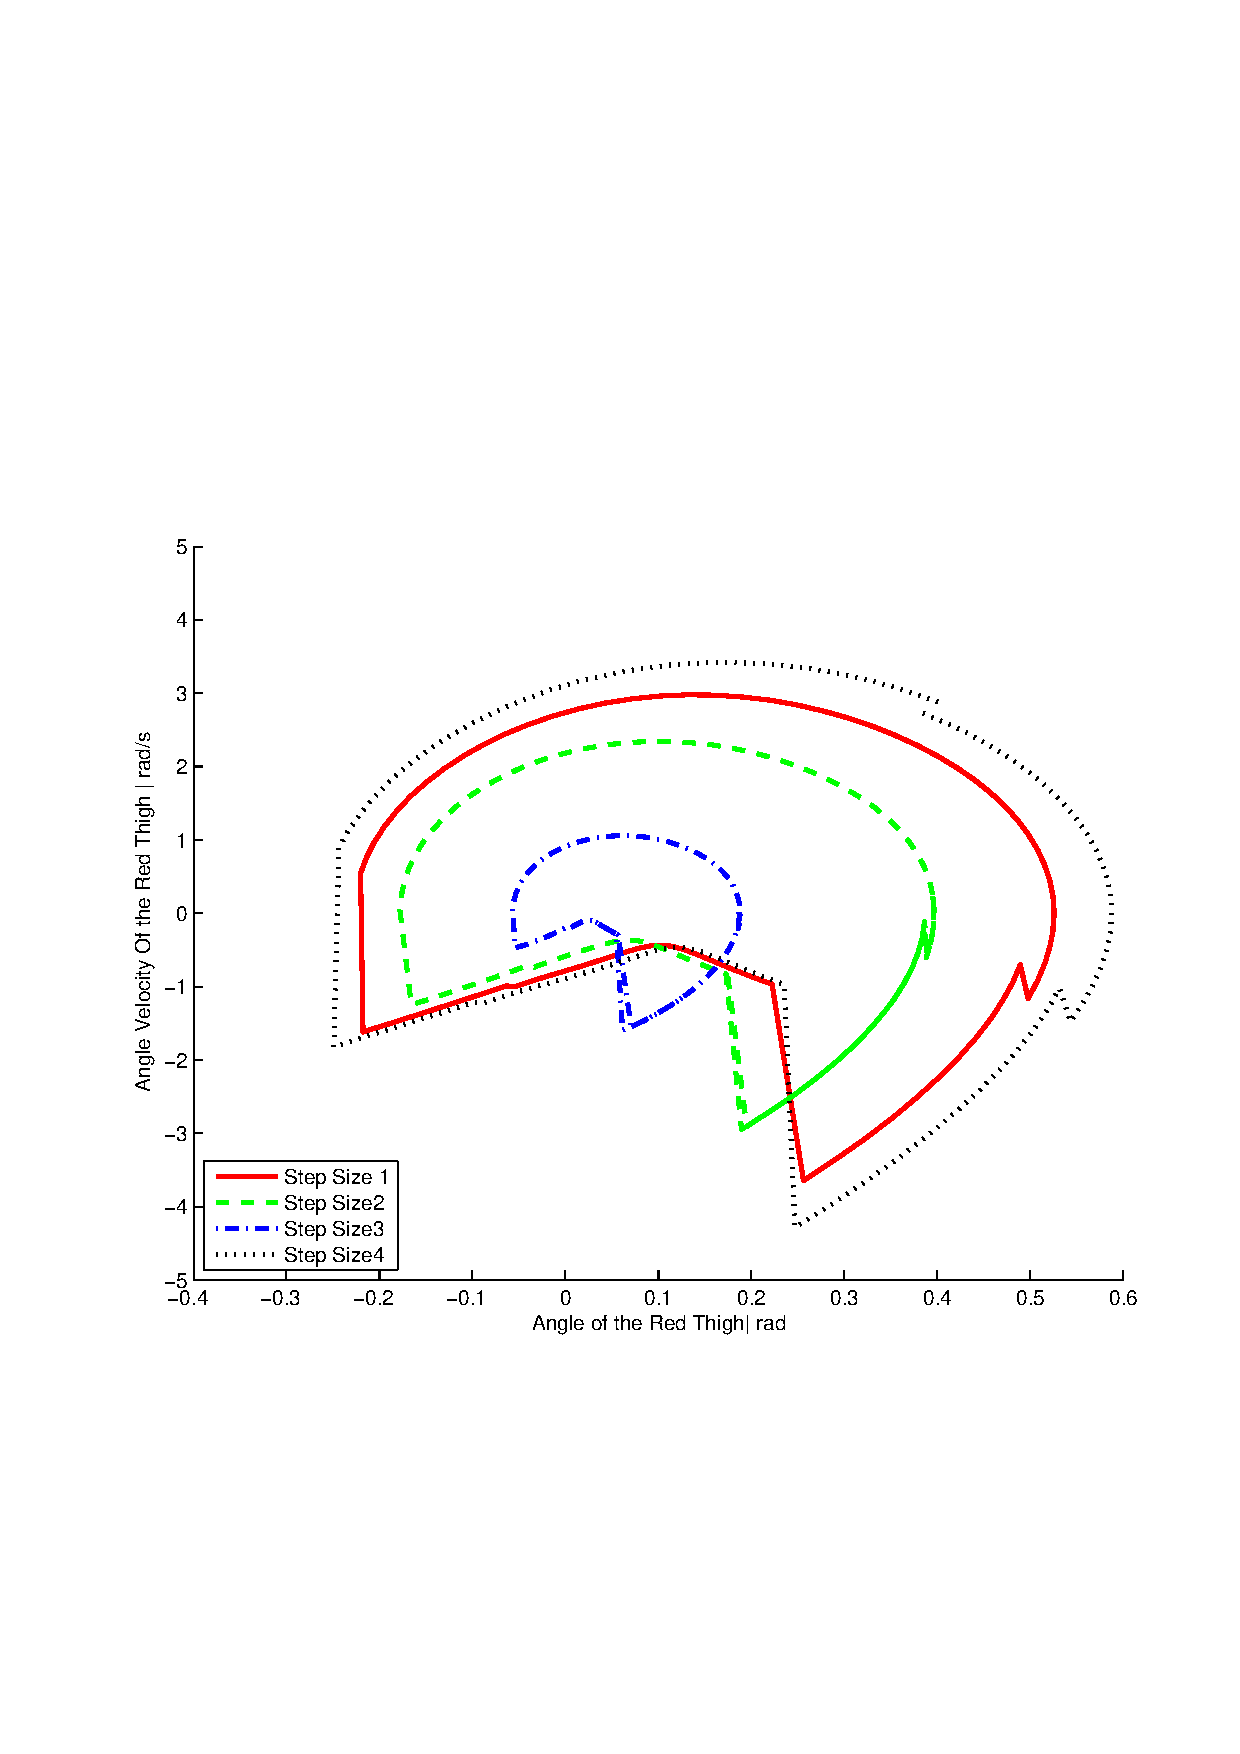
\includegraphics[width=0.7\textwidth]{DifferentStepSizeWalking}
    \fi
    \caption{different step size walking}
    \label{fig:differentlr}
\end{center}
\end{figure}


\begin{figure}[!htbp]
  \begin{center}
      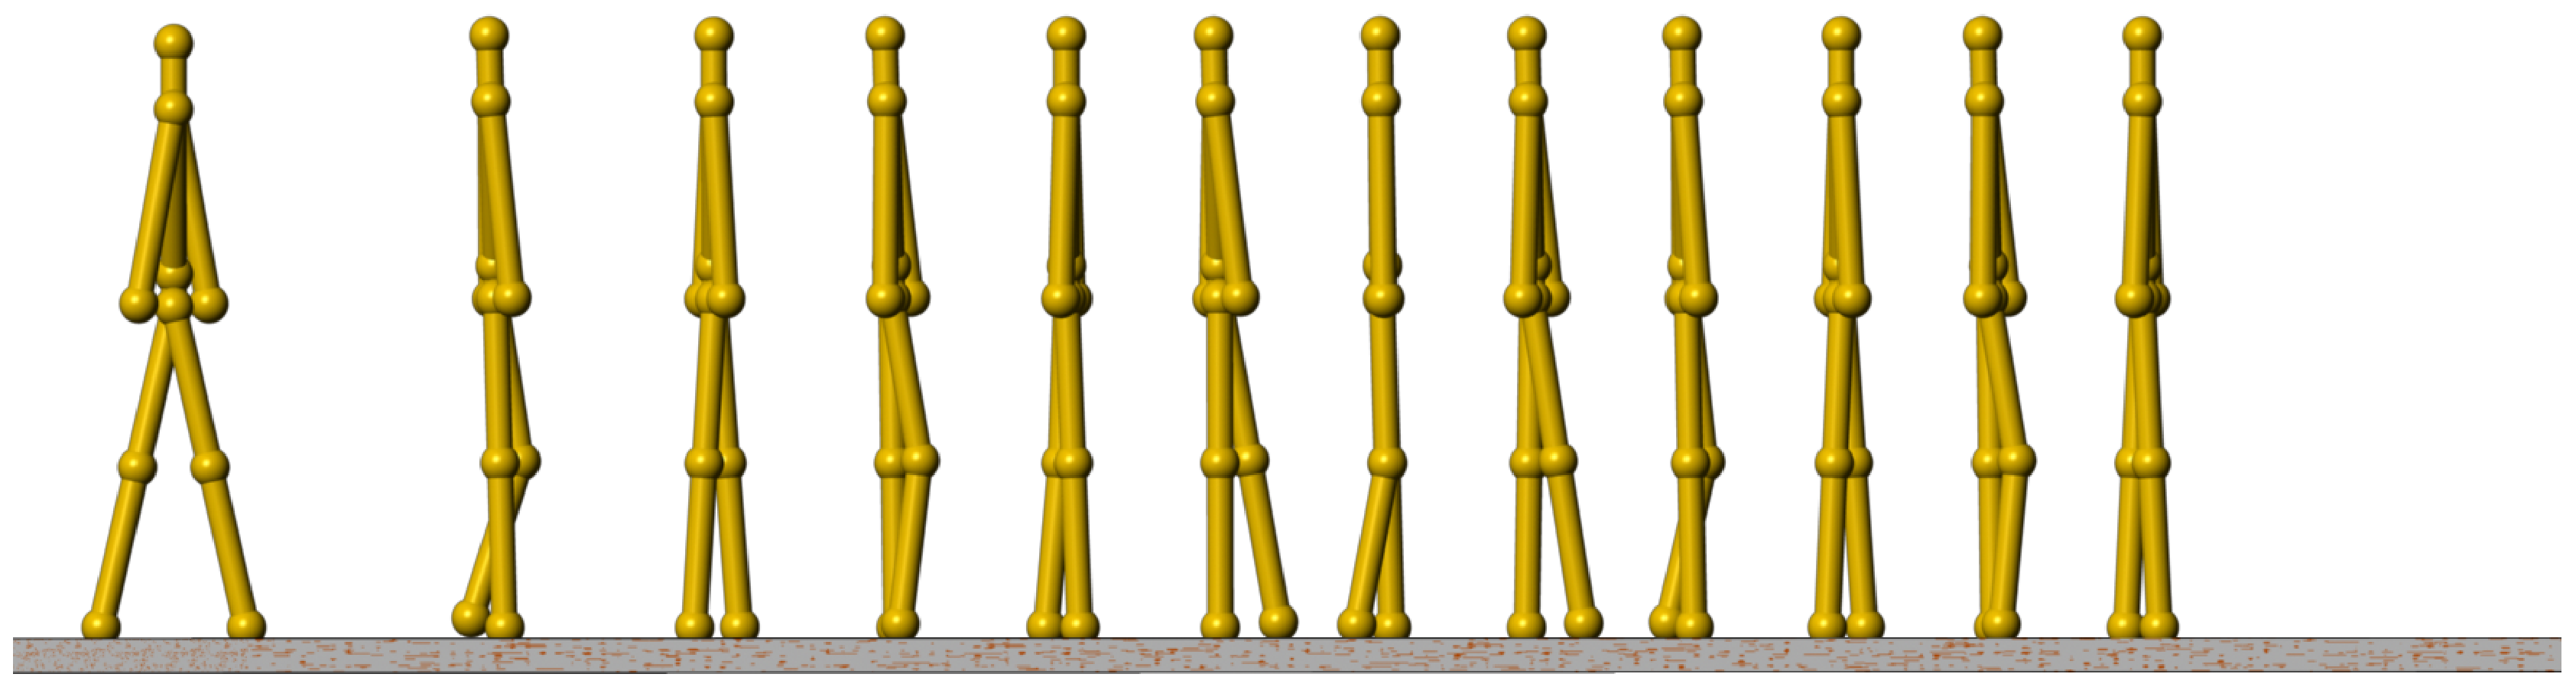
\includegraphics[width=0.7\textwidth]{walking_with_neural}
    \caption{Place Holder1}
    \label{fig:ss1}
\end{center}
\end{figure}

\begin{figure}[!htbp]
  \begin{center}
      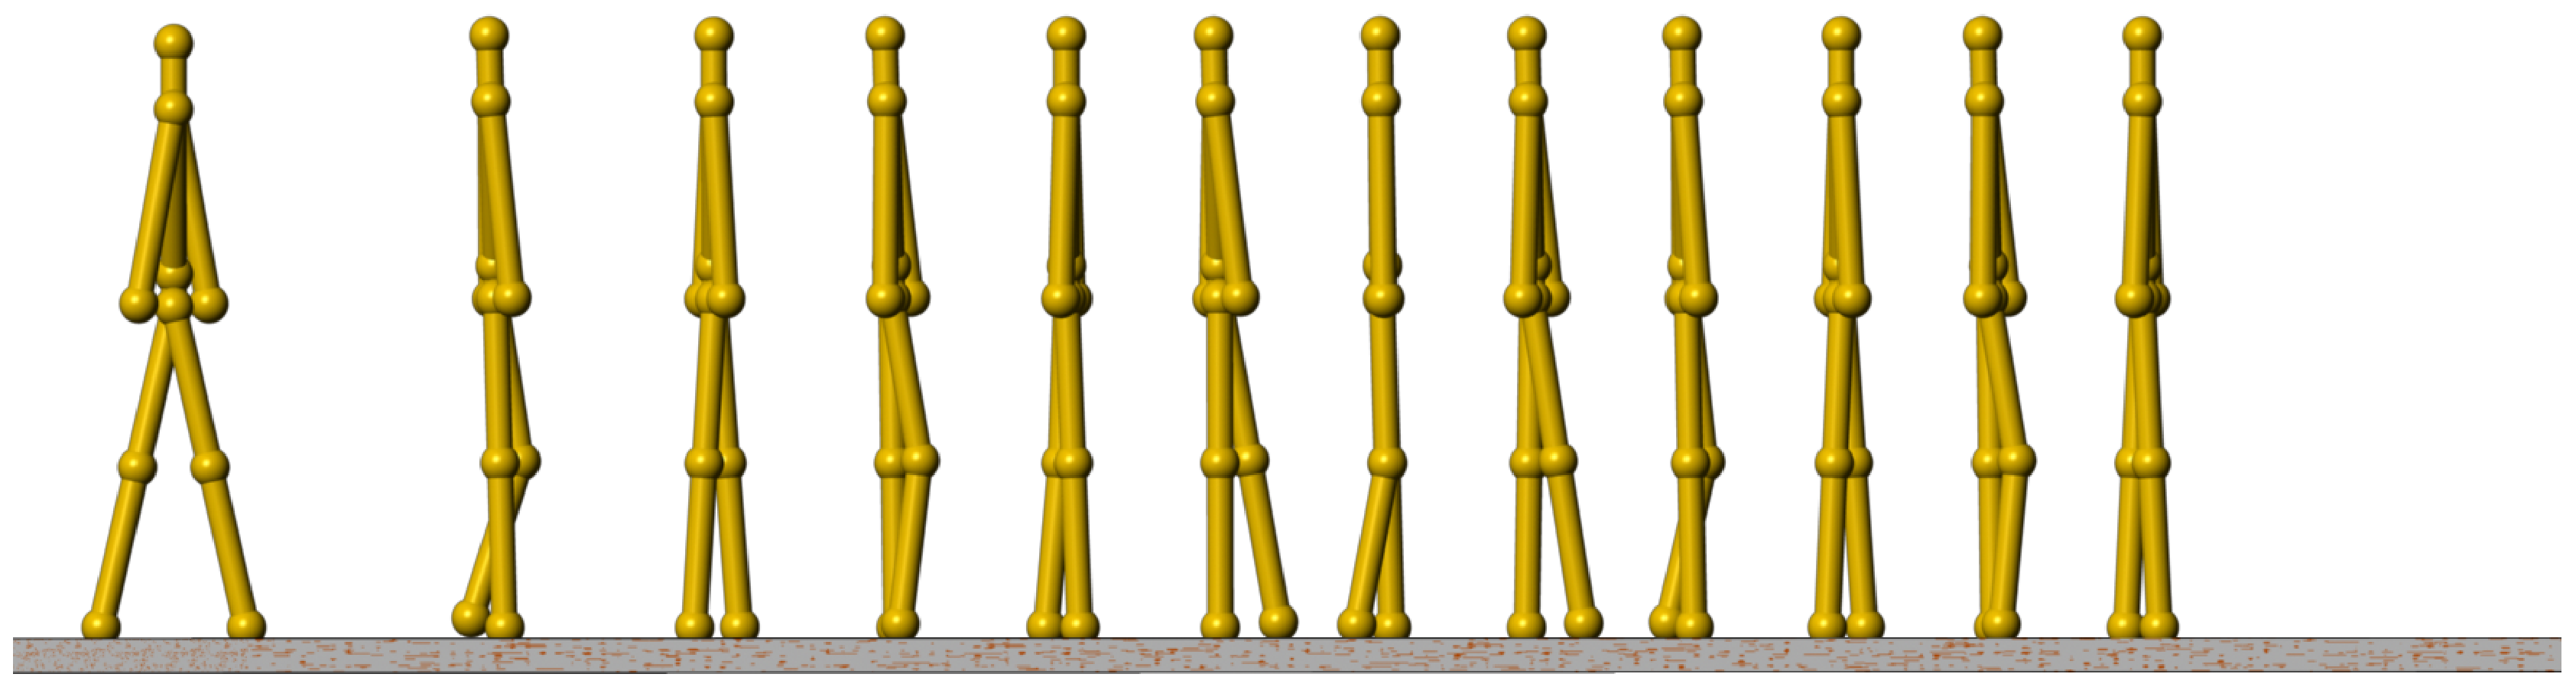
\includegraphics[width=0.7\textwidth]{walking_with_neural}
    \caption{Place Holder2}
    \label{fig:ss2}
\end{center}
\end{figure}

\begin{figure}[!htbp]
  \begin{center}
      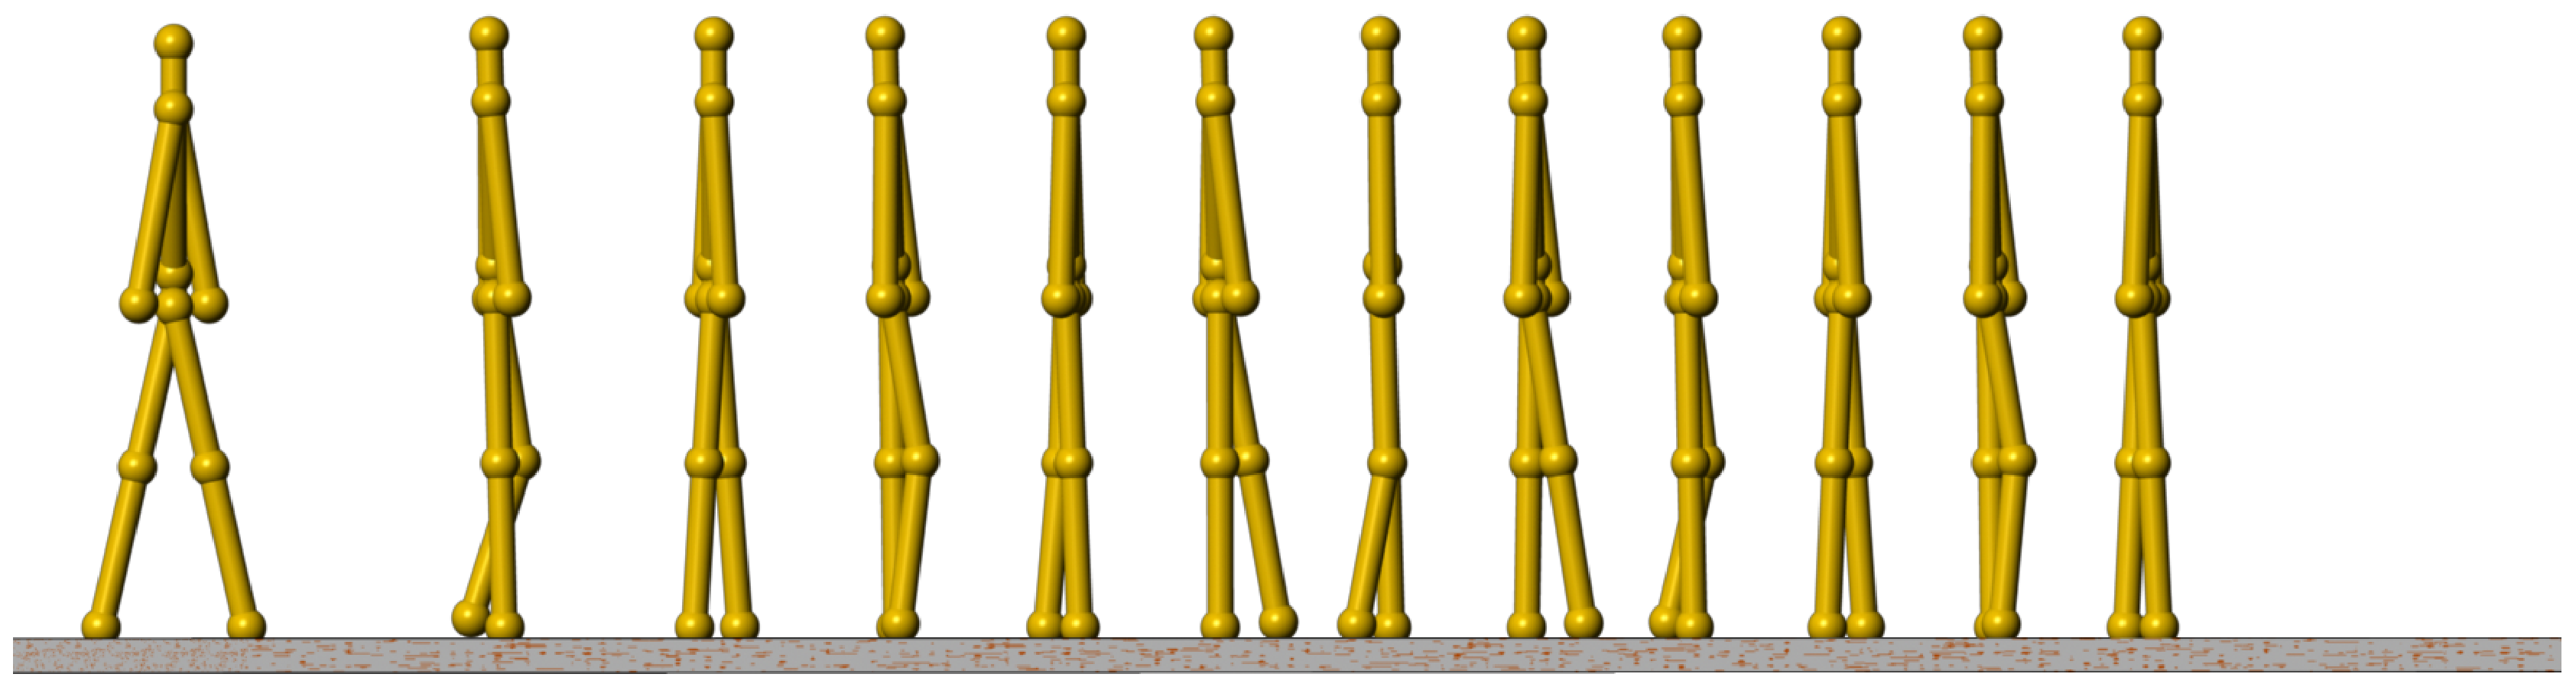
\includegraphics[width=0.7\textwidth]{walking_with_neural}
    \caption{Place Holder3}
    \label{fig:ss3}
\end{center}
\end{figure}




\subsubsection*{Different Leg Mass}
we also change the leg mass of the two leggs, make them not equal.
This will result two legs sway differently and the limit circle of original system is doubled.
Bigger difference will result in a gait looks like cripple.

\begin{figure}[!htbp]
  \begin{center}
    \leavevmode
    \ifpdf
      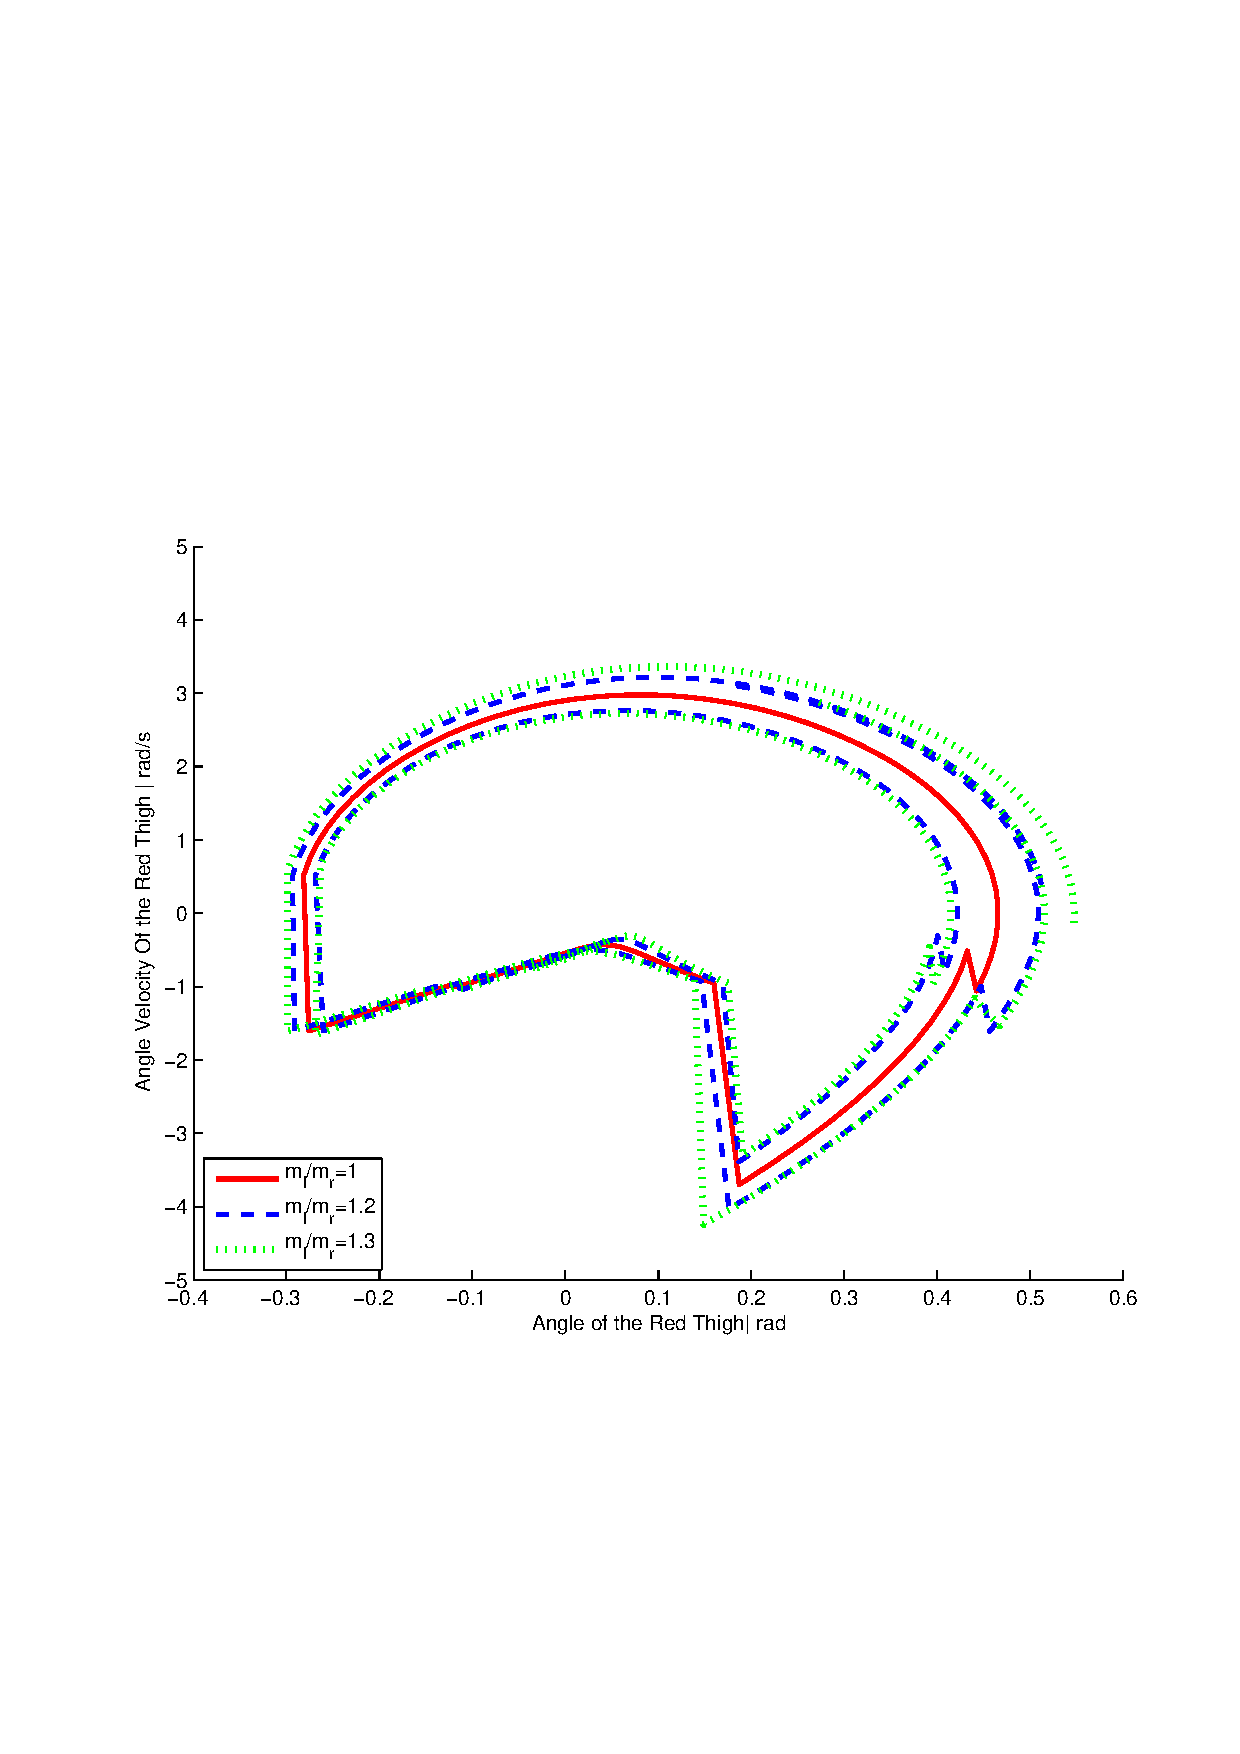
\includegraphics[height=6in]{DifferentLegMassLimitCircle}
    \else
      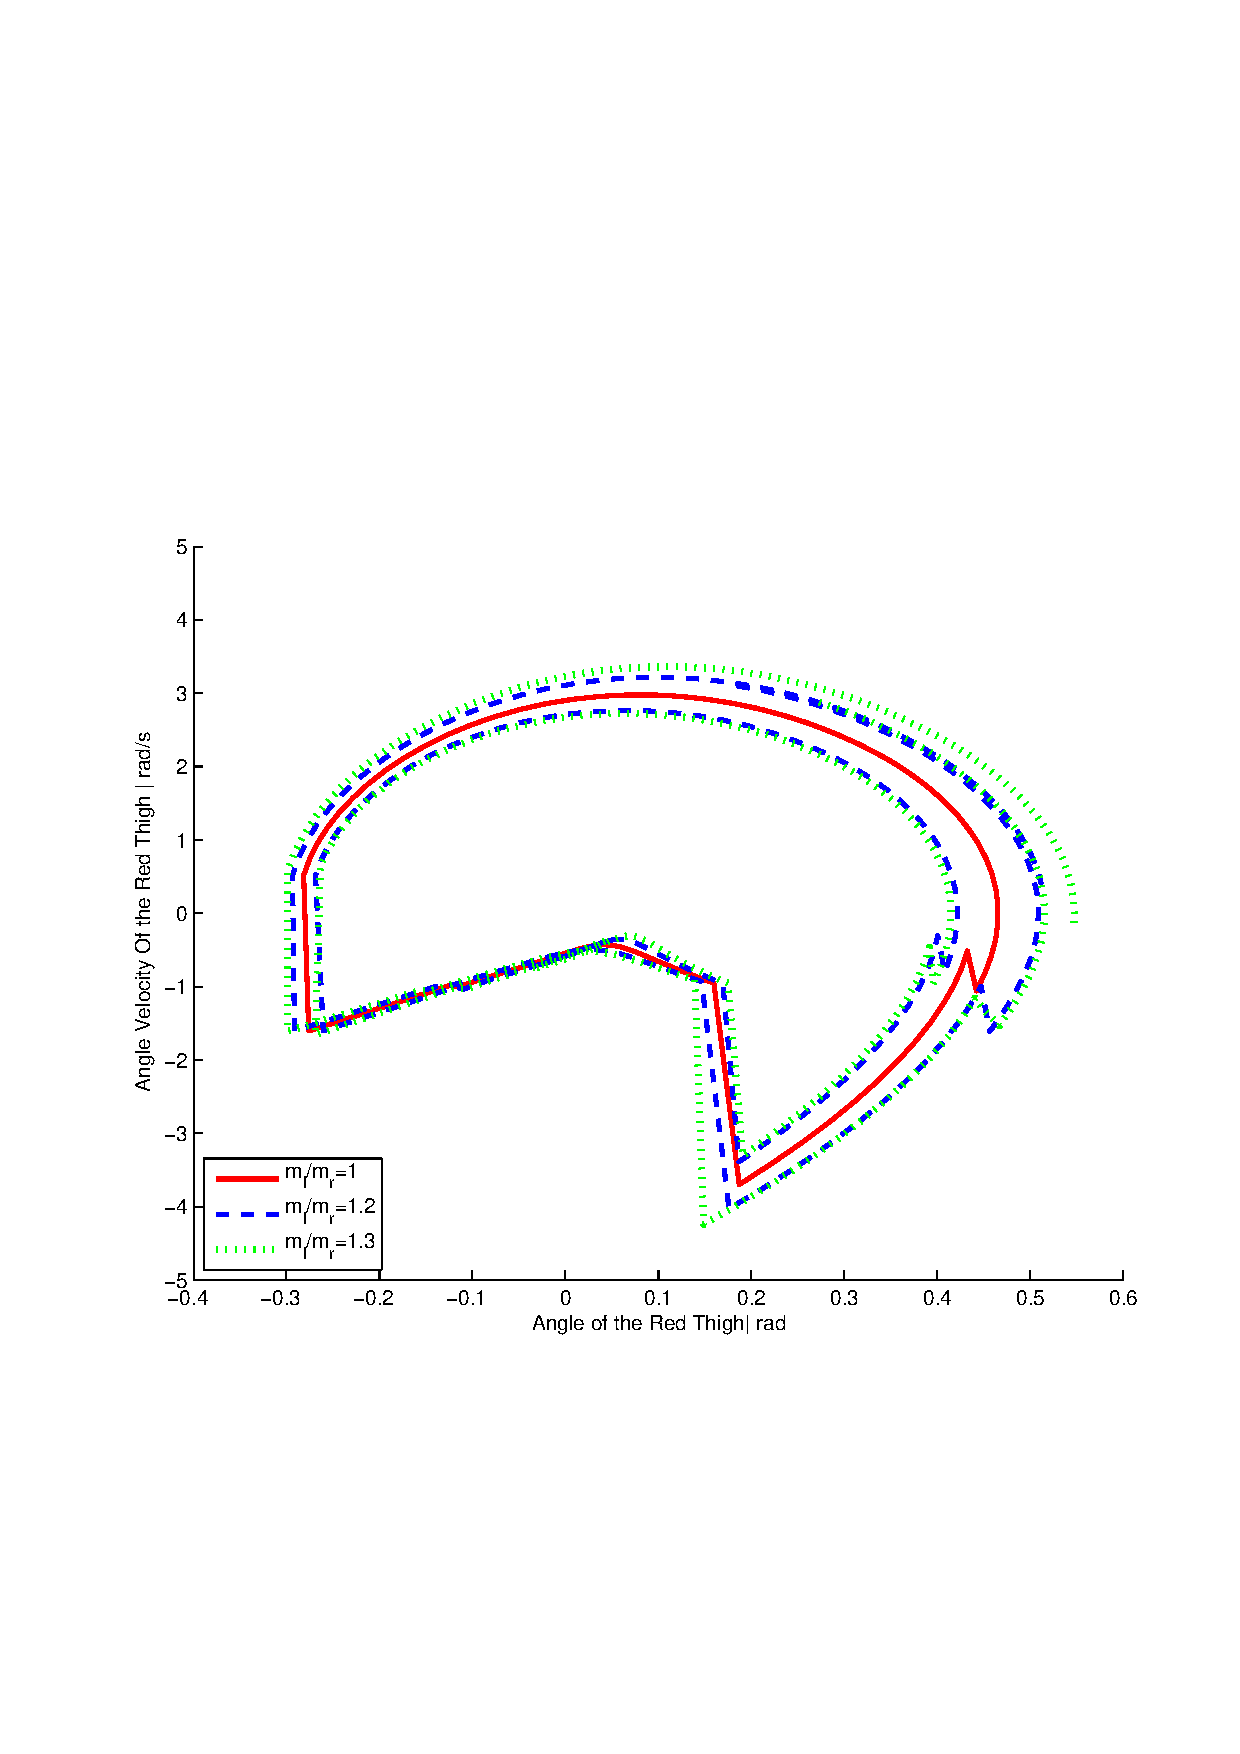
\includegraphics[width=0.7\textwidth]{DifferentLegMassLimitCircle}
    \fi
    \caption{Different Leg Mass Stable Gaits}
    \label{fig:differentlr}
\end{center}
\end{figure}


\begin{figure}[!htbp]
  \begin{center}
      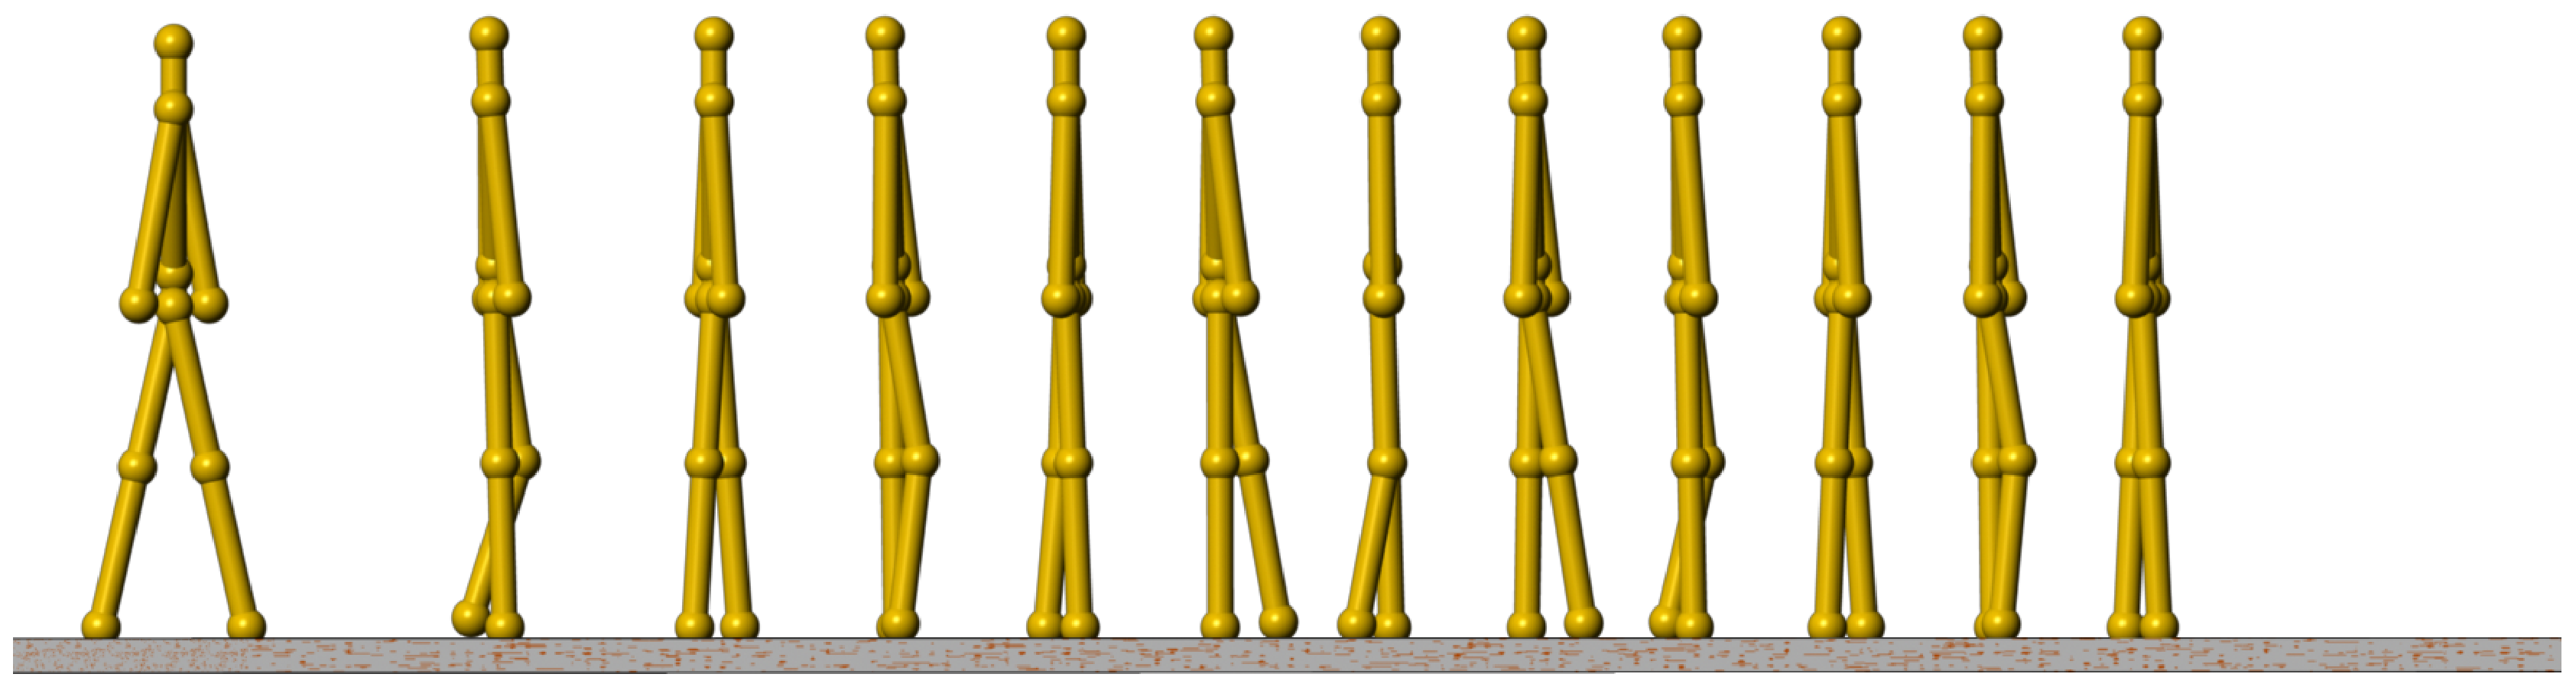
\includegraphics[width=0.7\textwidth]{walking_with_neural}
    \caption{Place Holder1}
    \label{fig:lm1}
\end{center}
\end{figure}

\begin{figure}[!htbp]
  \begin{center}
      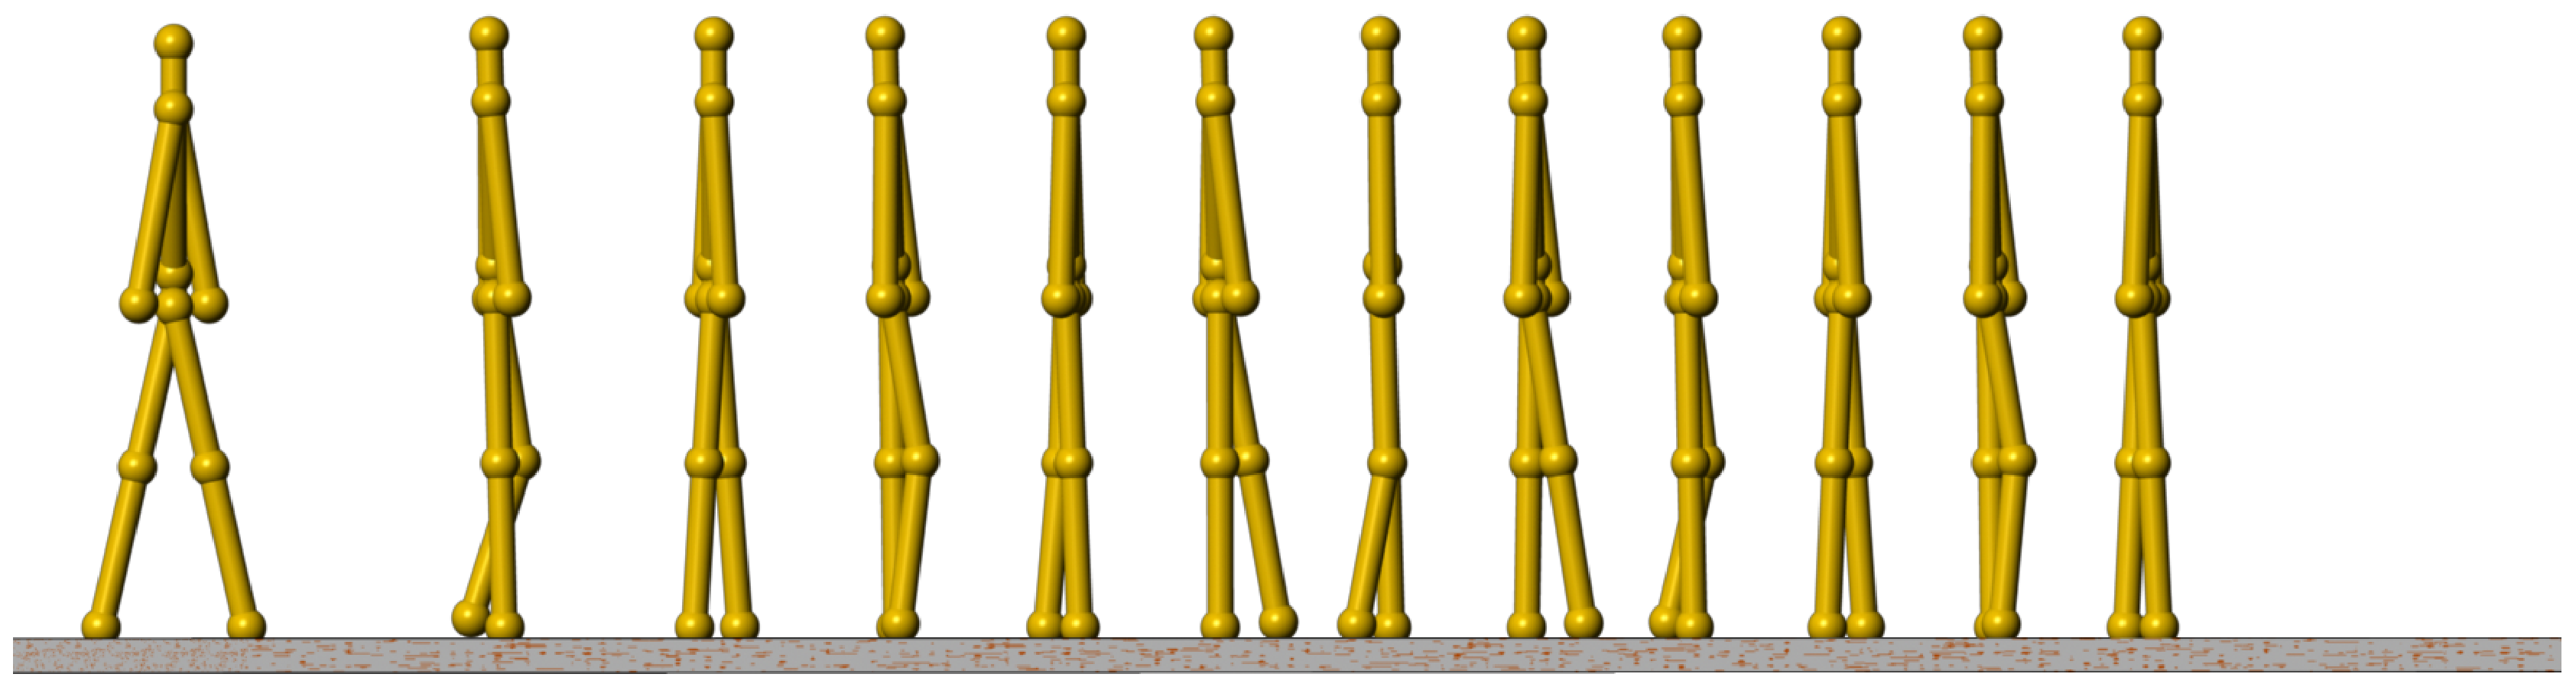
\includegraphics[width=0.7\textwidth]{walking_with_neural}
    \caption{Place Holder2}
    \label{fig:lm2}
\end{center}
\end{figure}

\begin{figure}[!htbp]
  \begin{center}
      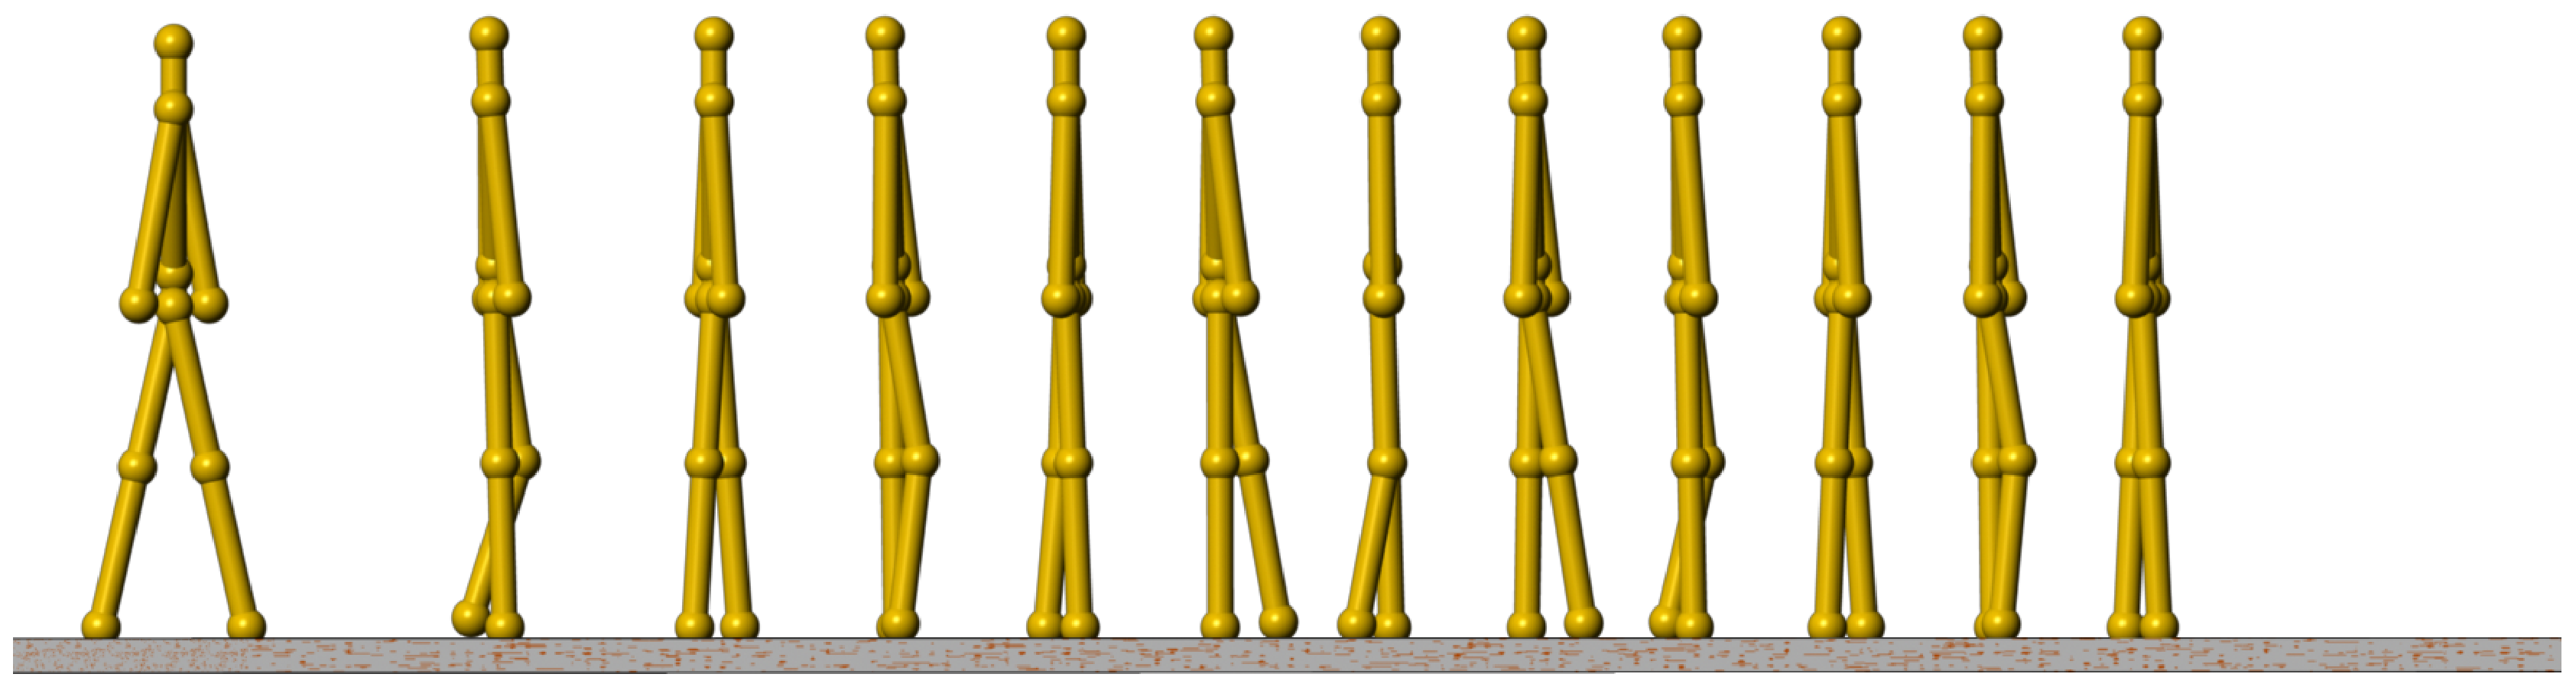
\includegraphics[width=0.7\textwidth]{walking_with_neural}
    \caption{Place Holder3}
    \label{fig:lm3}
\end{center}
\end{figure}


%lmass/rmass=1

%lmass/rmass=0.75


the period is double and the step is not symmetrical any more. So the two legs move in a slight different manner, but still, it keeps walking.

\section{Transform Gait Adaptation}
Local Invariant Controller will not generate different gait style, but it will transform the gait at different speed and at different terrain.
One important limitation we find of limit cycle is it can not walk up slope.
This is because when walking upslope, it is symmetrical to walk down the slope in another direction, if the limit cycle is stable enough, after a few steps, it will walk backwards and walk down slope.


the failure of walking up slope is show in figure

\begin{figure}[!htbp]
  \begin{center}
      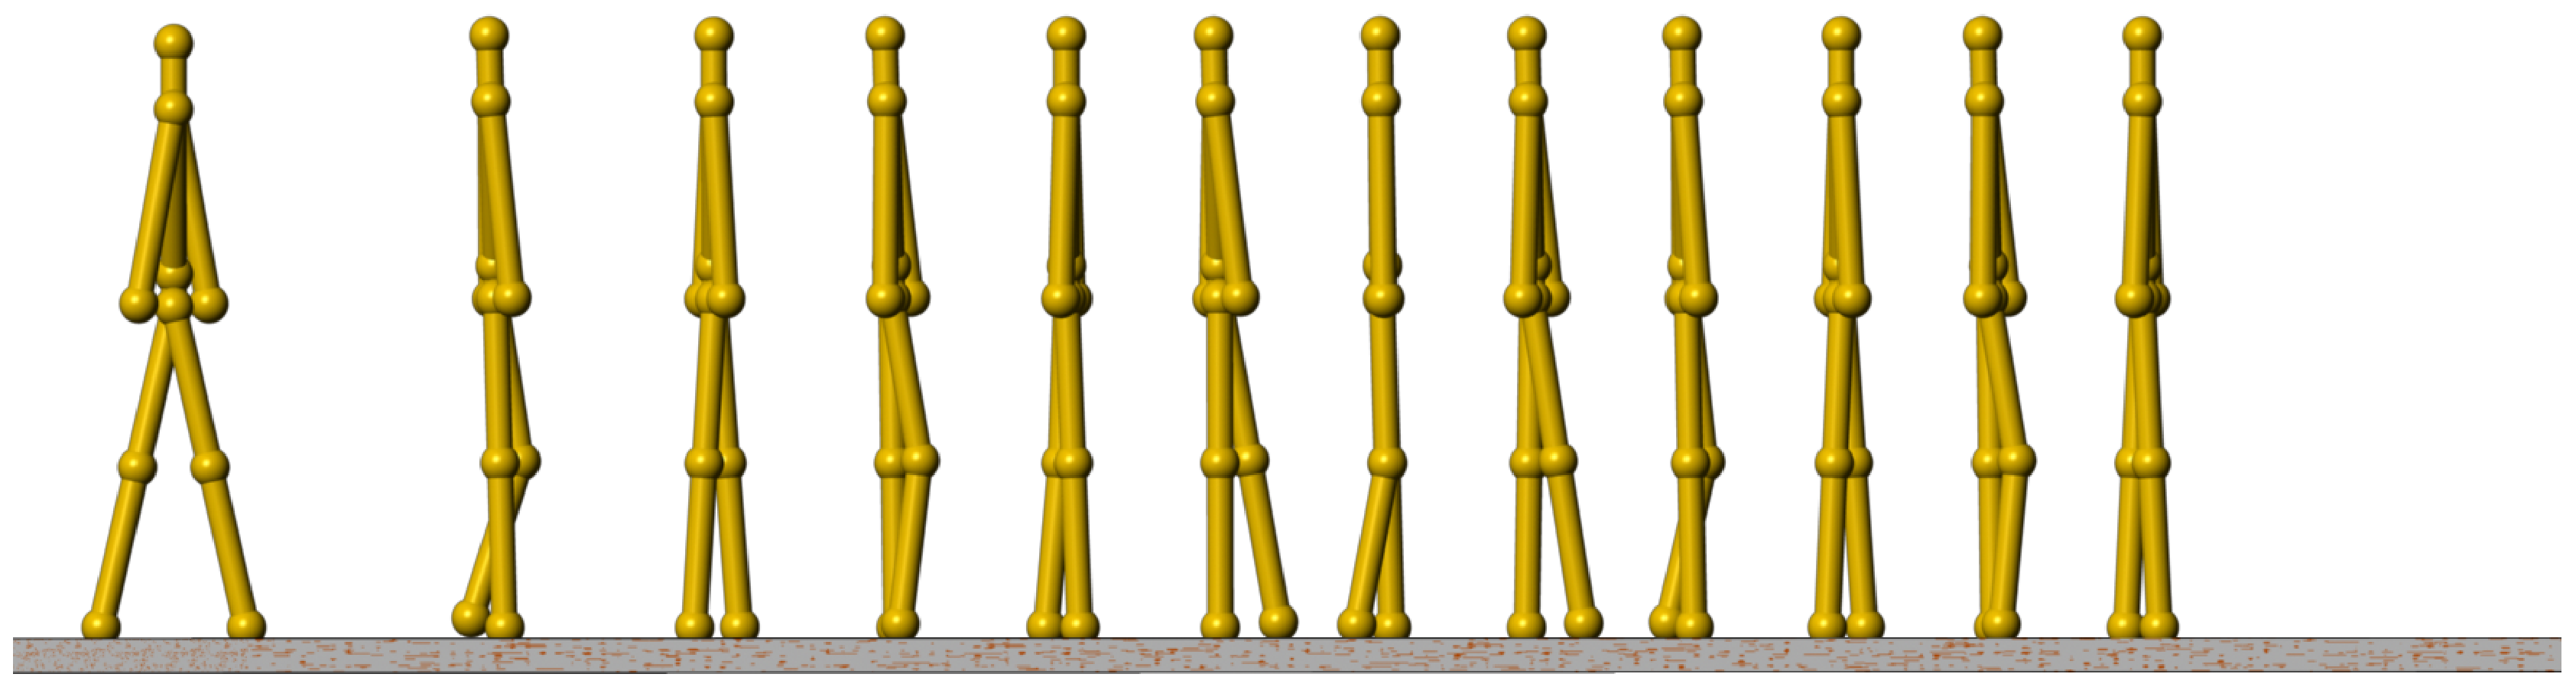
\includegraphics[width=0.7\textwidth]{walking_with_neural}
    \caption{Place Holder}
    \label{fig:withoutlocalcontroller}
\end{center}
\end{figure}

we apply two types of local motor invariant.
\begin{itemize}

\HiItem{Slope Change}.
Slope Change is incorporate through offset transformation.

%N=N*g.
\[
\ulocal=N(\mathrm{cos}(\alpha)-1)
\]
\HiItem{Speed Change}
Speed Action will ajust the walking speed, but maintain the walking gait.
the the new walking speed is $s$.
we have
\[  
\ulocal=N(\alpha^2-1)
\]
\end{itemize}

\begin{figure}[!htbp]
  \begin{center}
    \leavevmode
    \ifpdf
      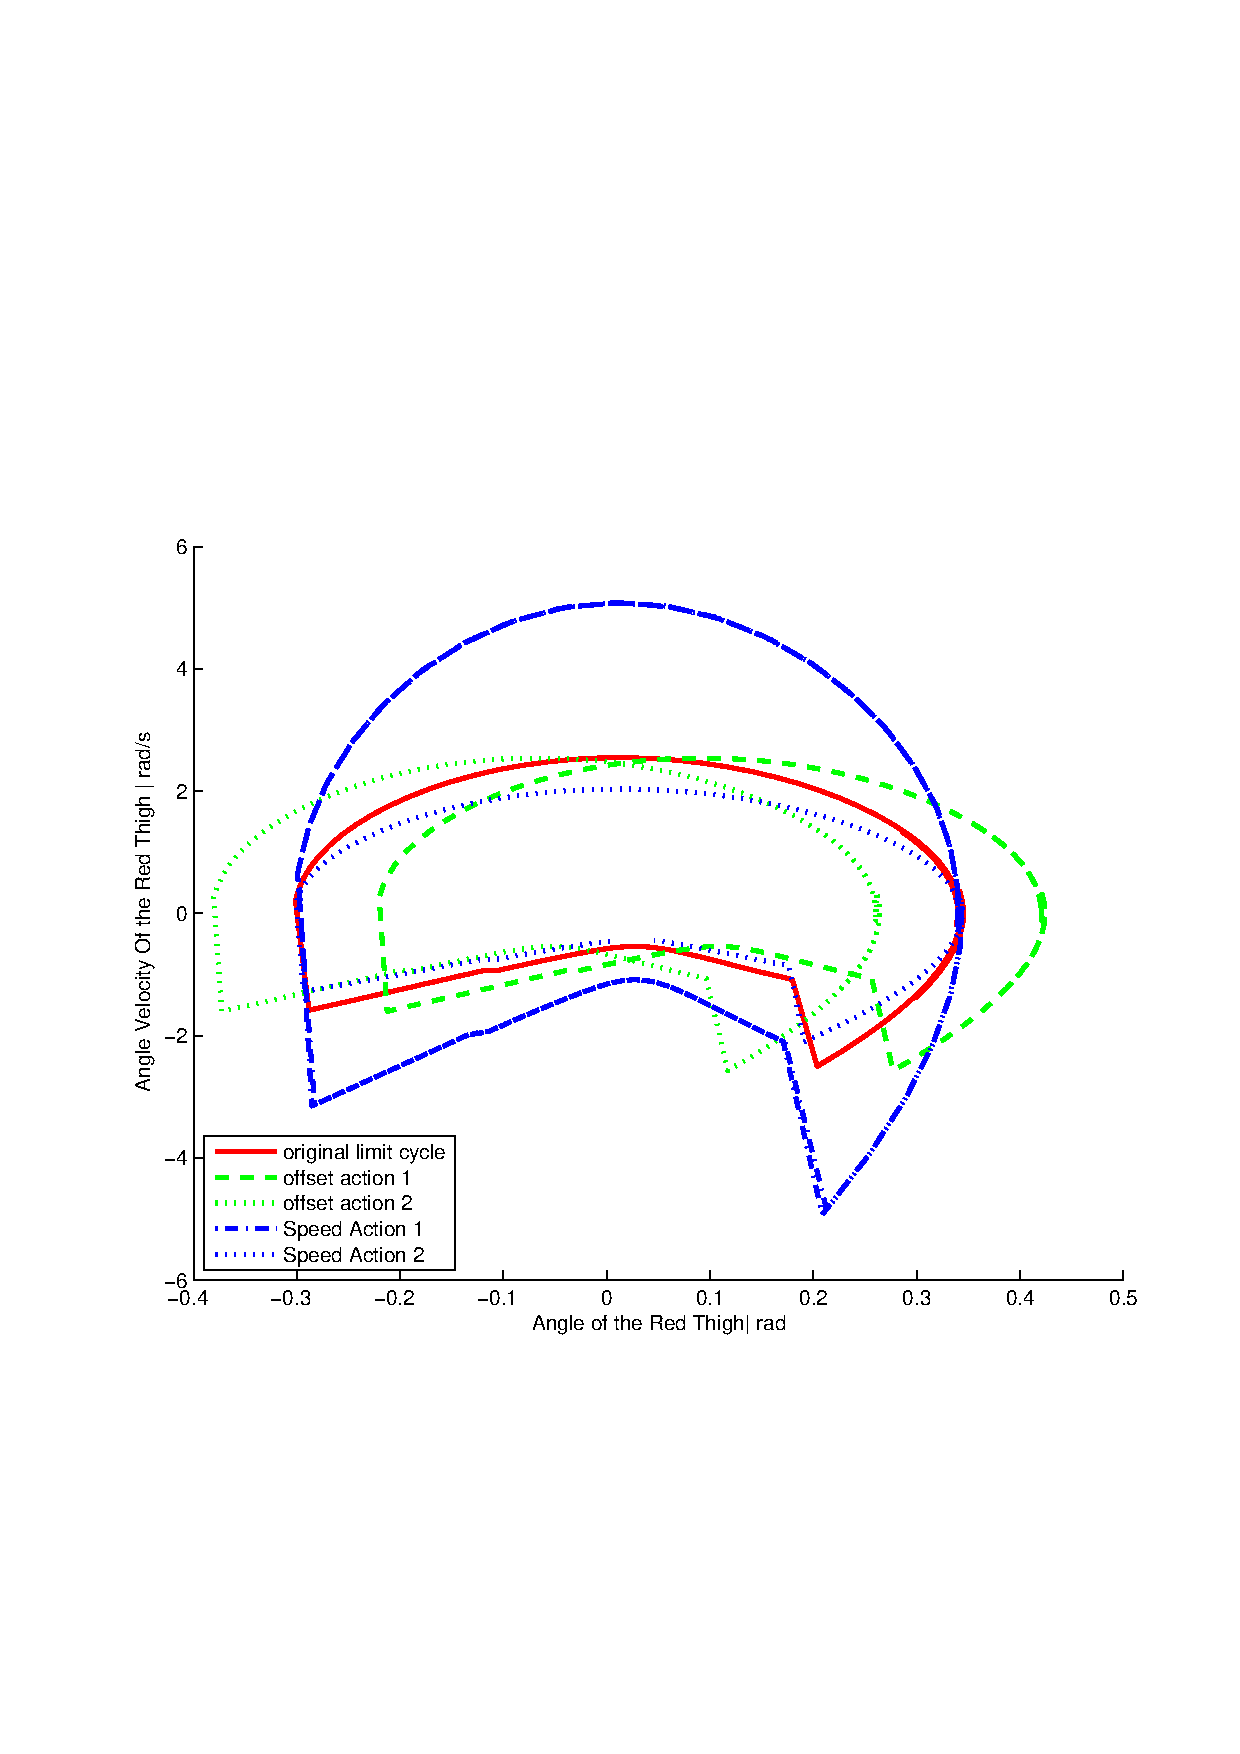
\includegraphics[height=6in]{LieGroupAction}
    \else
      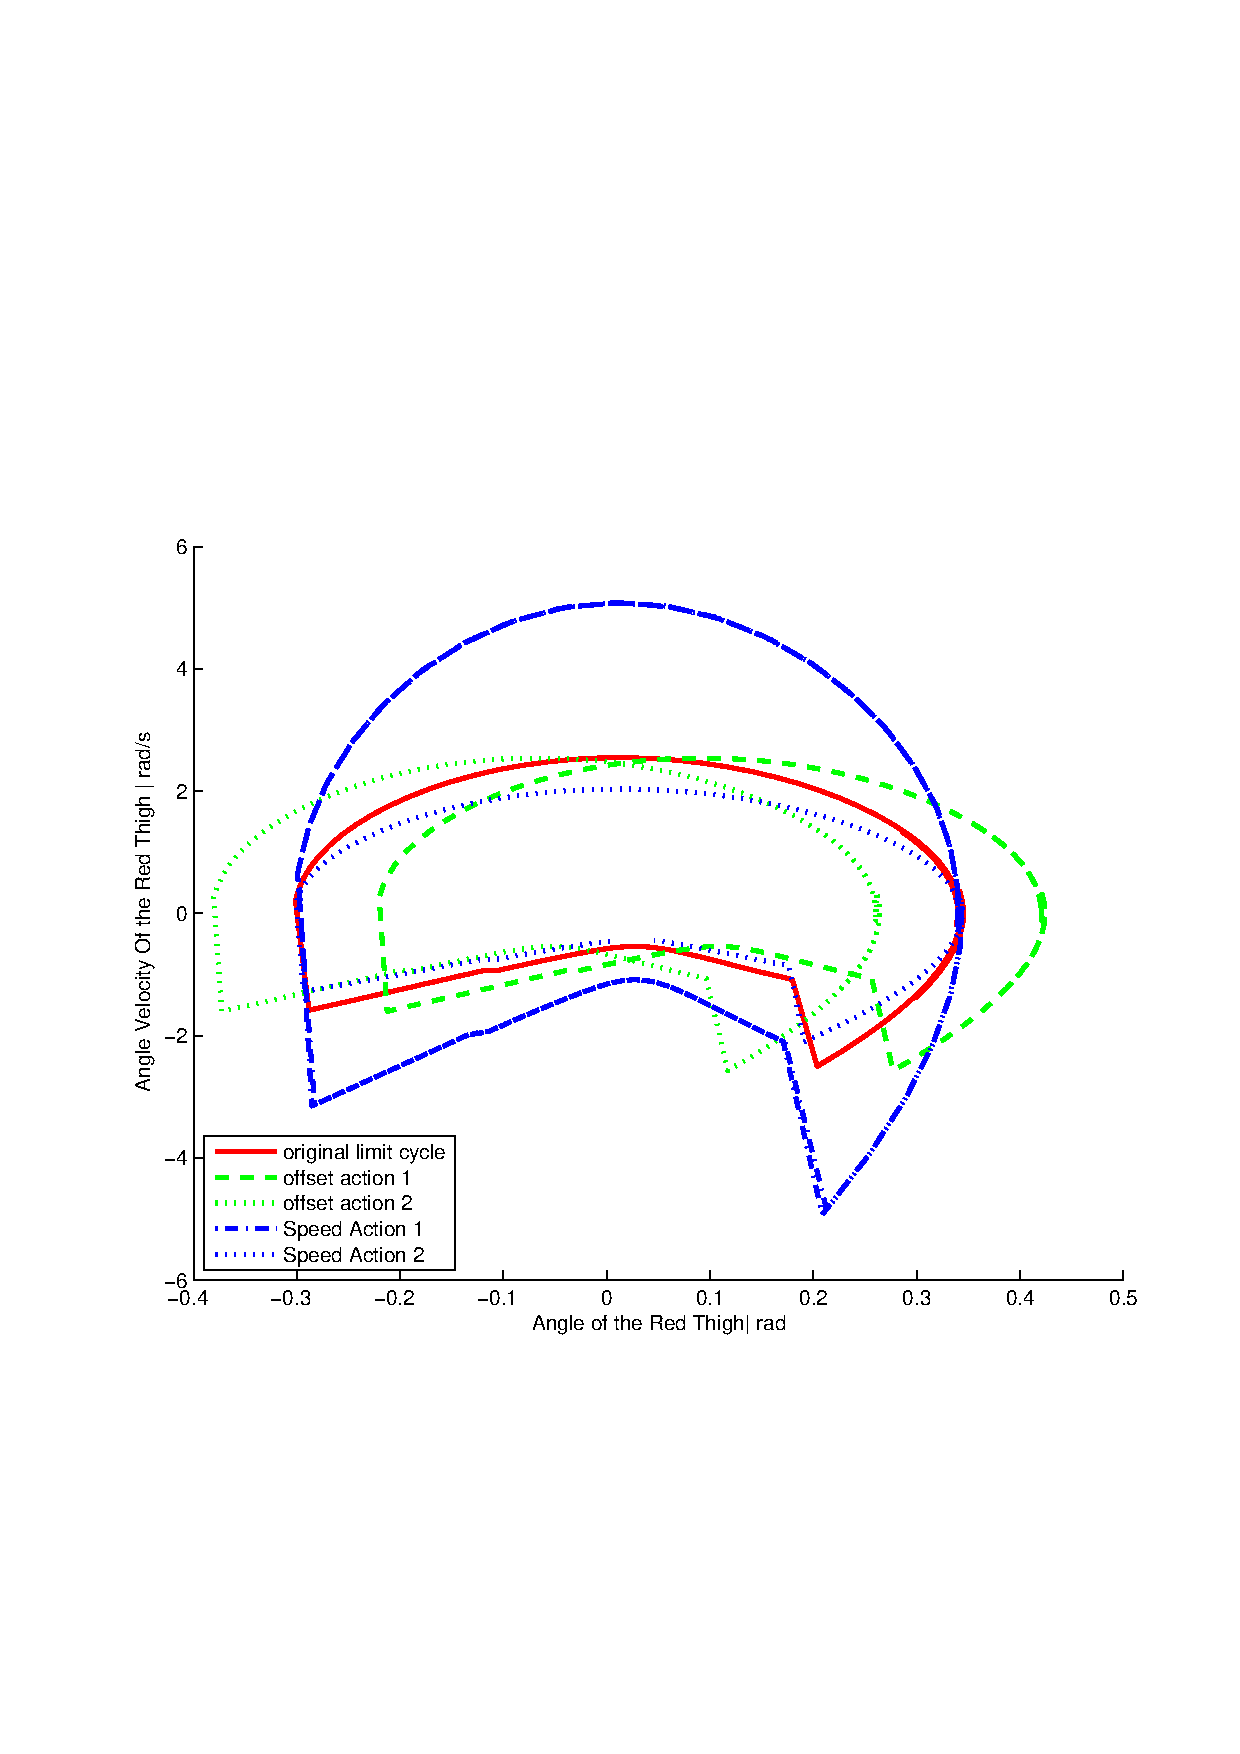
\includegraphics[width=0.7\textwidth]{LieGroupAction}
    \fi
    \caption{Different Leg Mass Stable Gaits}
    \label{fig:differentlr}
\end{center}
\end{figure}

The red on is the original limit cycle.
Green one are apply speed action
Blue ones are applied  locol transform action

Also it can help the passive walker walk upslope.
as show in figure


\begin{figure}[!htbp]
  \begin{center}
    \leavevmode
    \ifpdf
      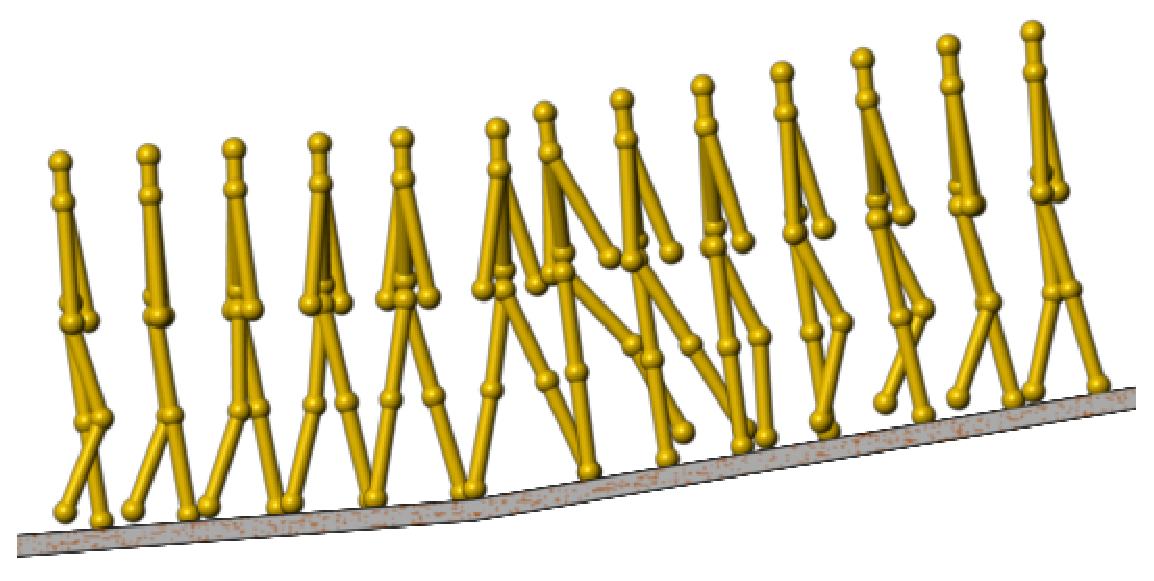
\includegraphics[height=6in]{walking_local_control}
    \else
      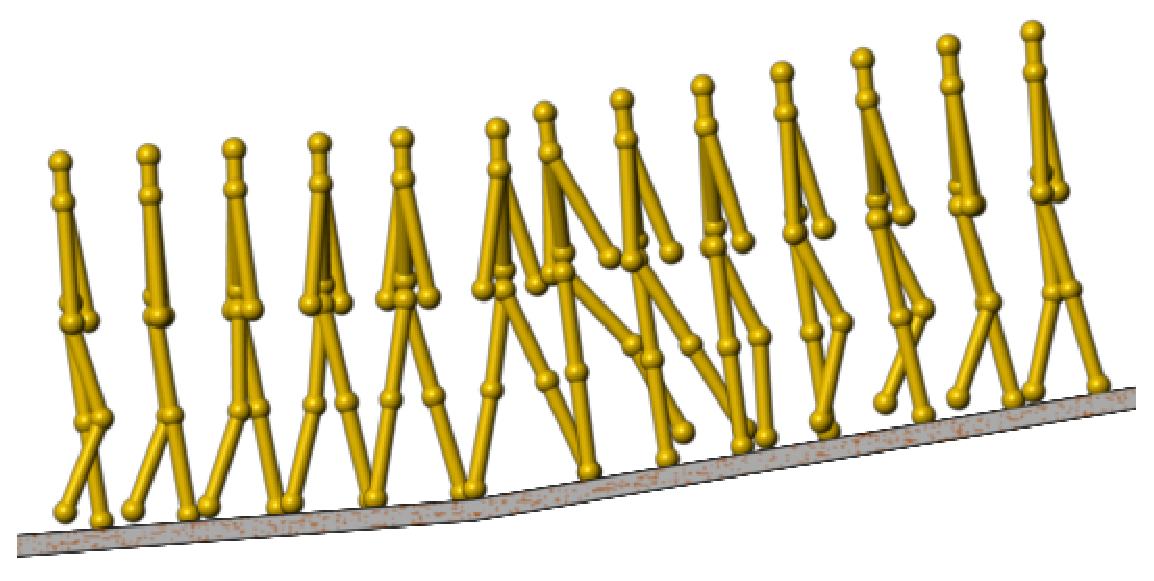
\includegraphics[width=0.7\textwidth]{walking_local_control}
    \fi
    \caption{Varying Terrain}
    \label{fig:diffterrain}
\end{center}
\end{figure}




\begin{figure}[!htbp]
  \begin{center}
    \leavevmode
    \ifpdf
      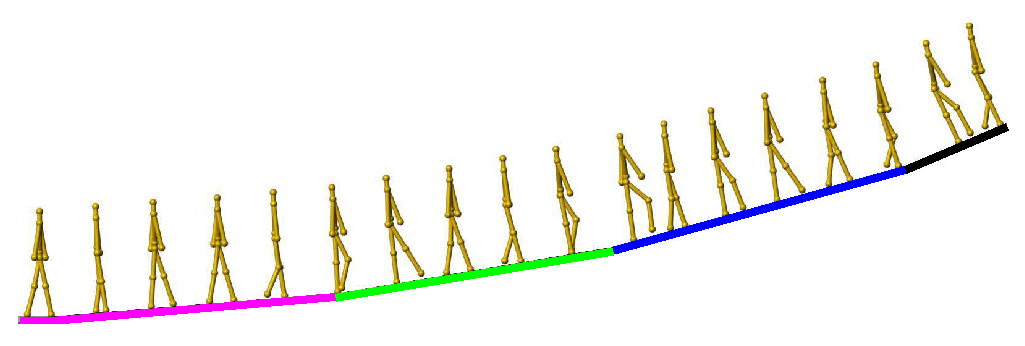
\includegraphics[height=6in]{walk_terrain_anim}
    \else
      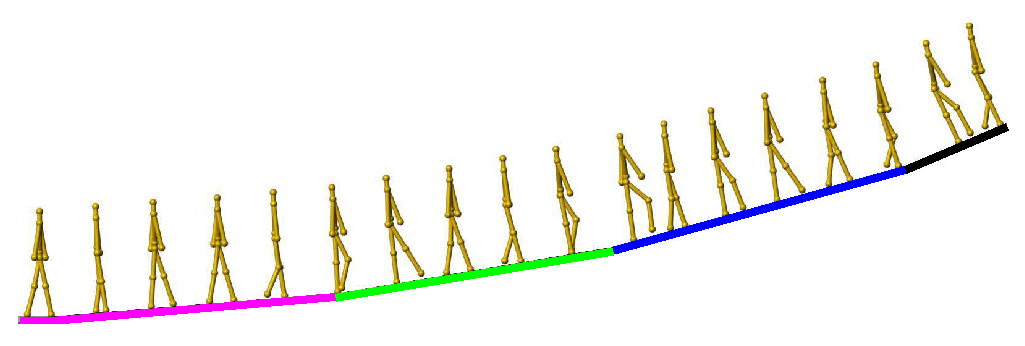
\includegraphics[width=0.7\textwidth]{walk_terrain_anim}
    \fi
    \caption{Varying Terrain}
    \label{fig:diffterrain}
\end{center}
\end{figure}



and on phase plot we see

\begin{figure}[!htbp]
  \begin{center}
    \leavevmode
    \ifpdf
      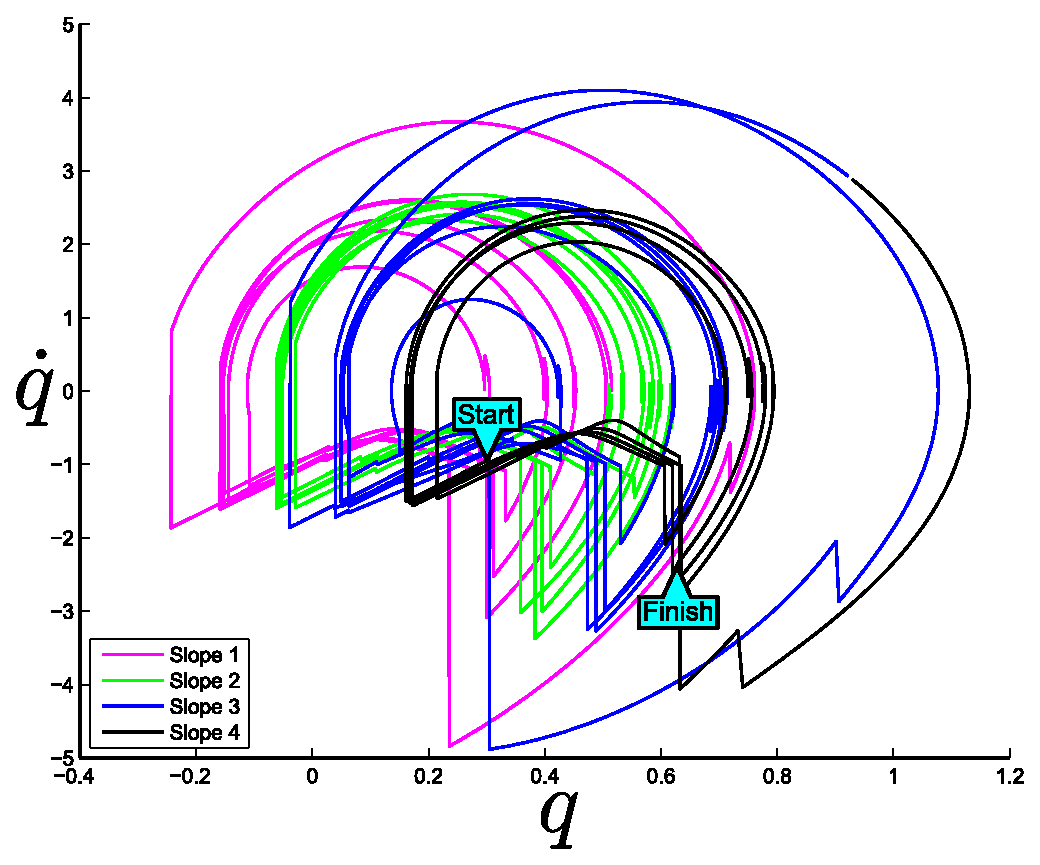
\includegraphics[height=6in]{walk_terrain}
    \else
      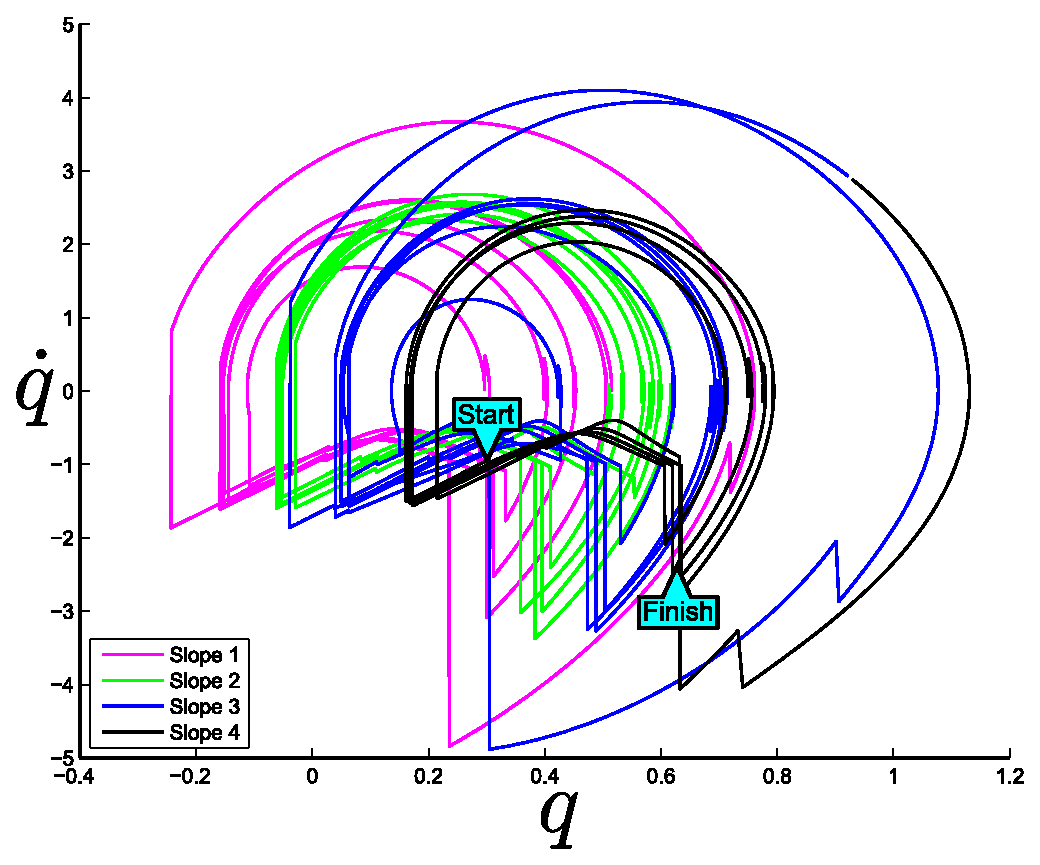
\includegraphics[width=0.7\textwidth]{walk_terrain}
    \fi
    \caption{Varying Terrain}
    \label{fig:diffterrainphase}
\end{center}
\end{figure}

and another terrain.
\begin{figure}[!htbp]
  \begin{center}
    \leavevmode
    \ifpdf
      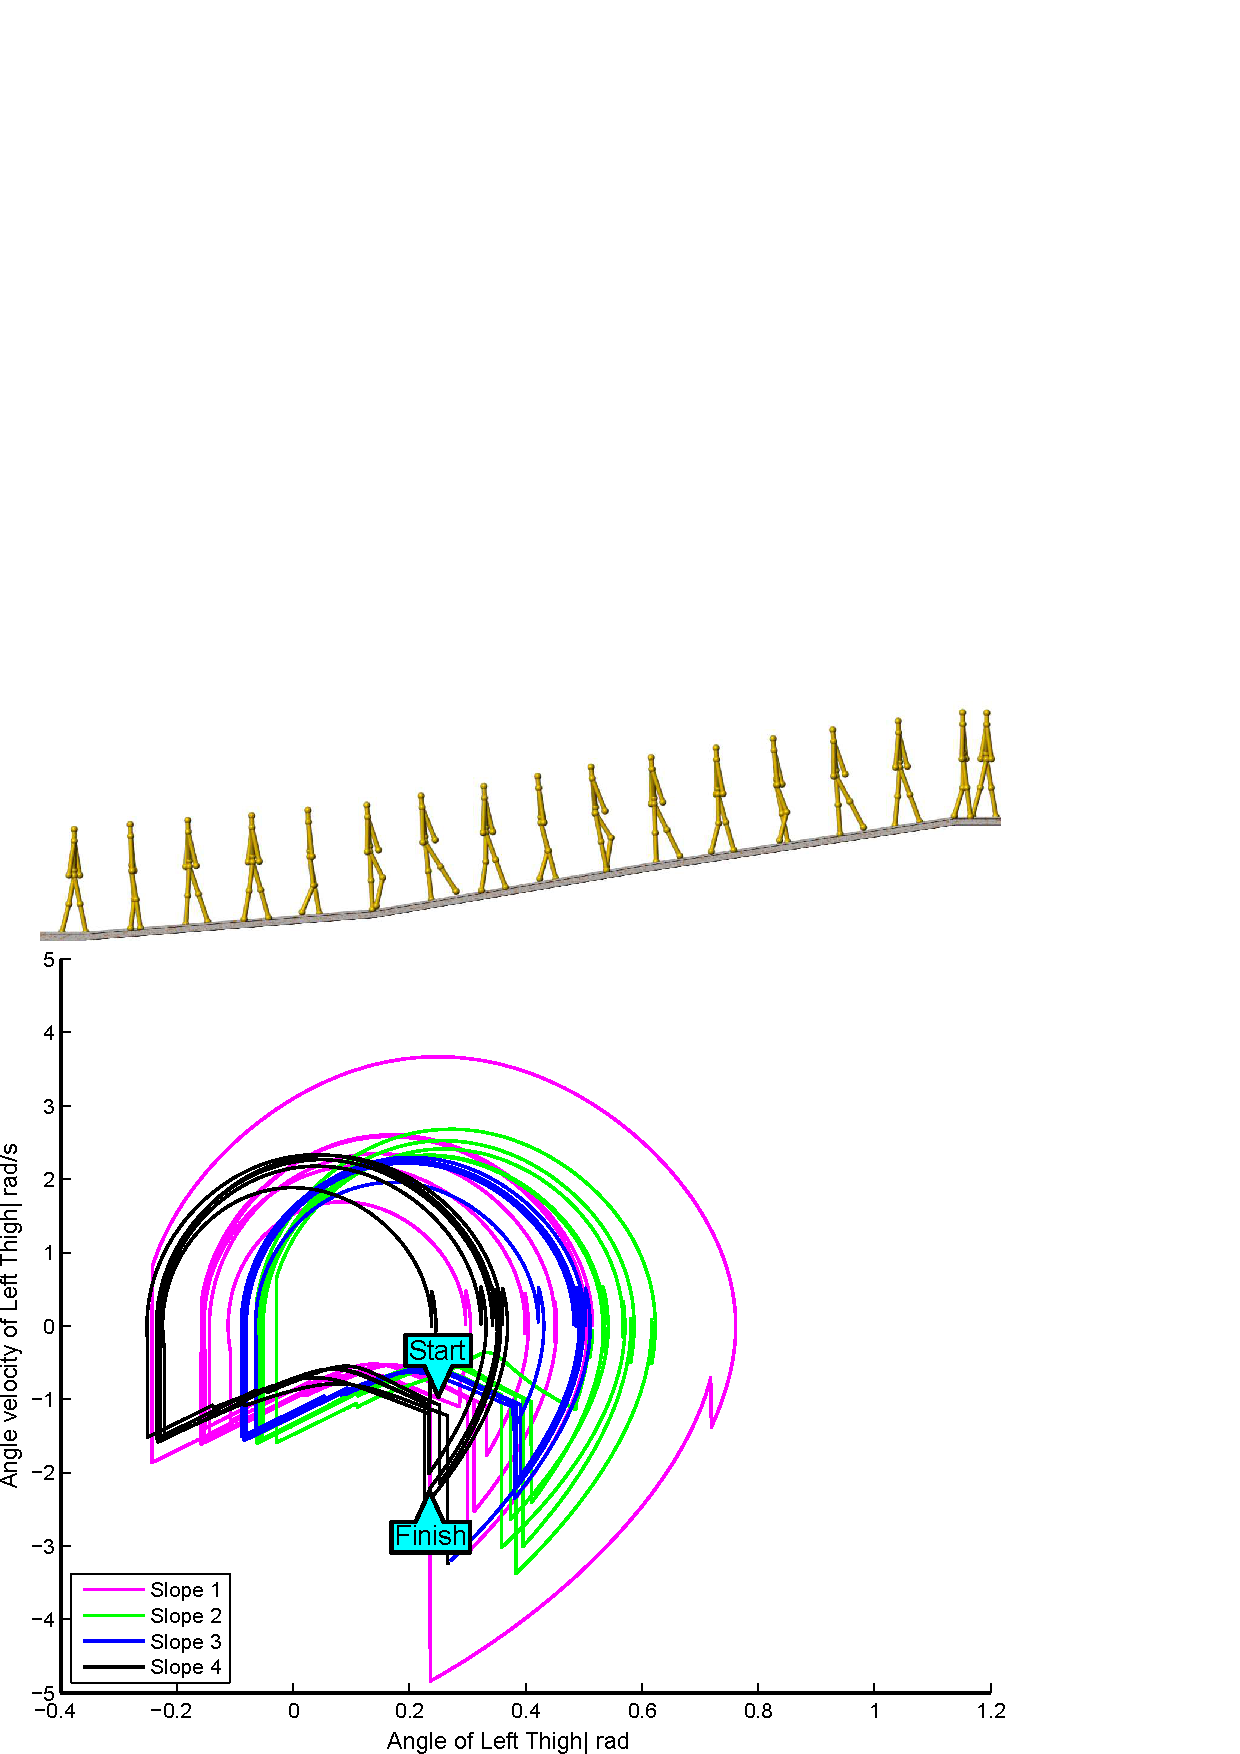
\includegraphics[height=6in]{walk_terrain2}
    \else
      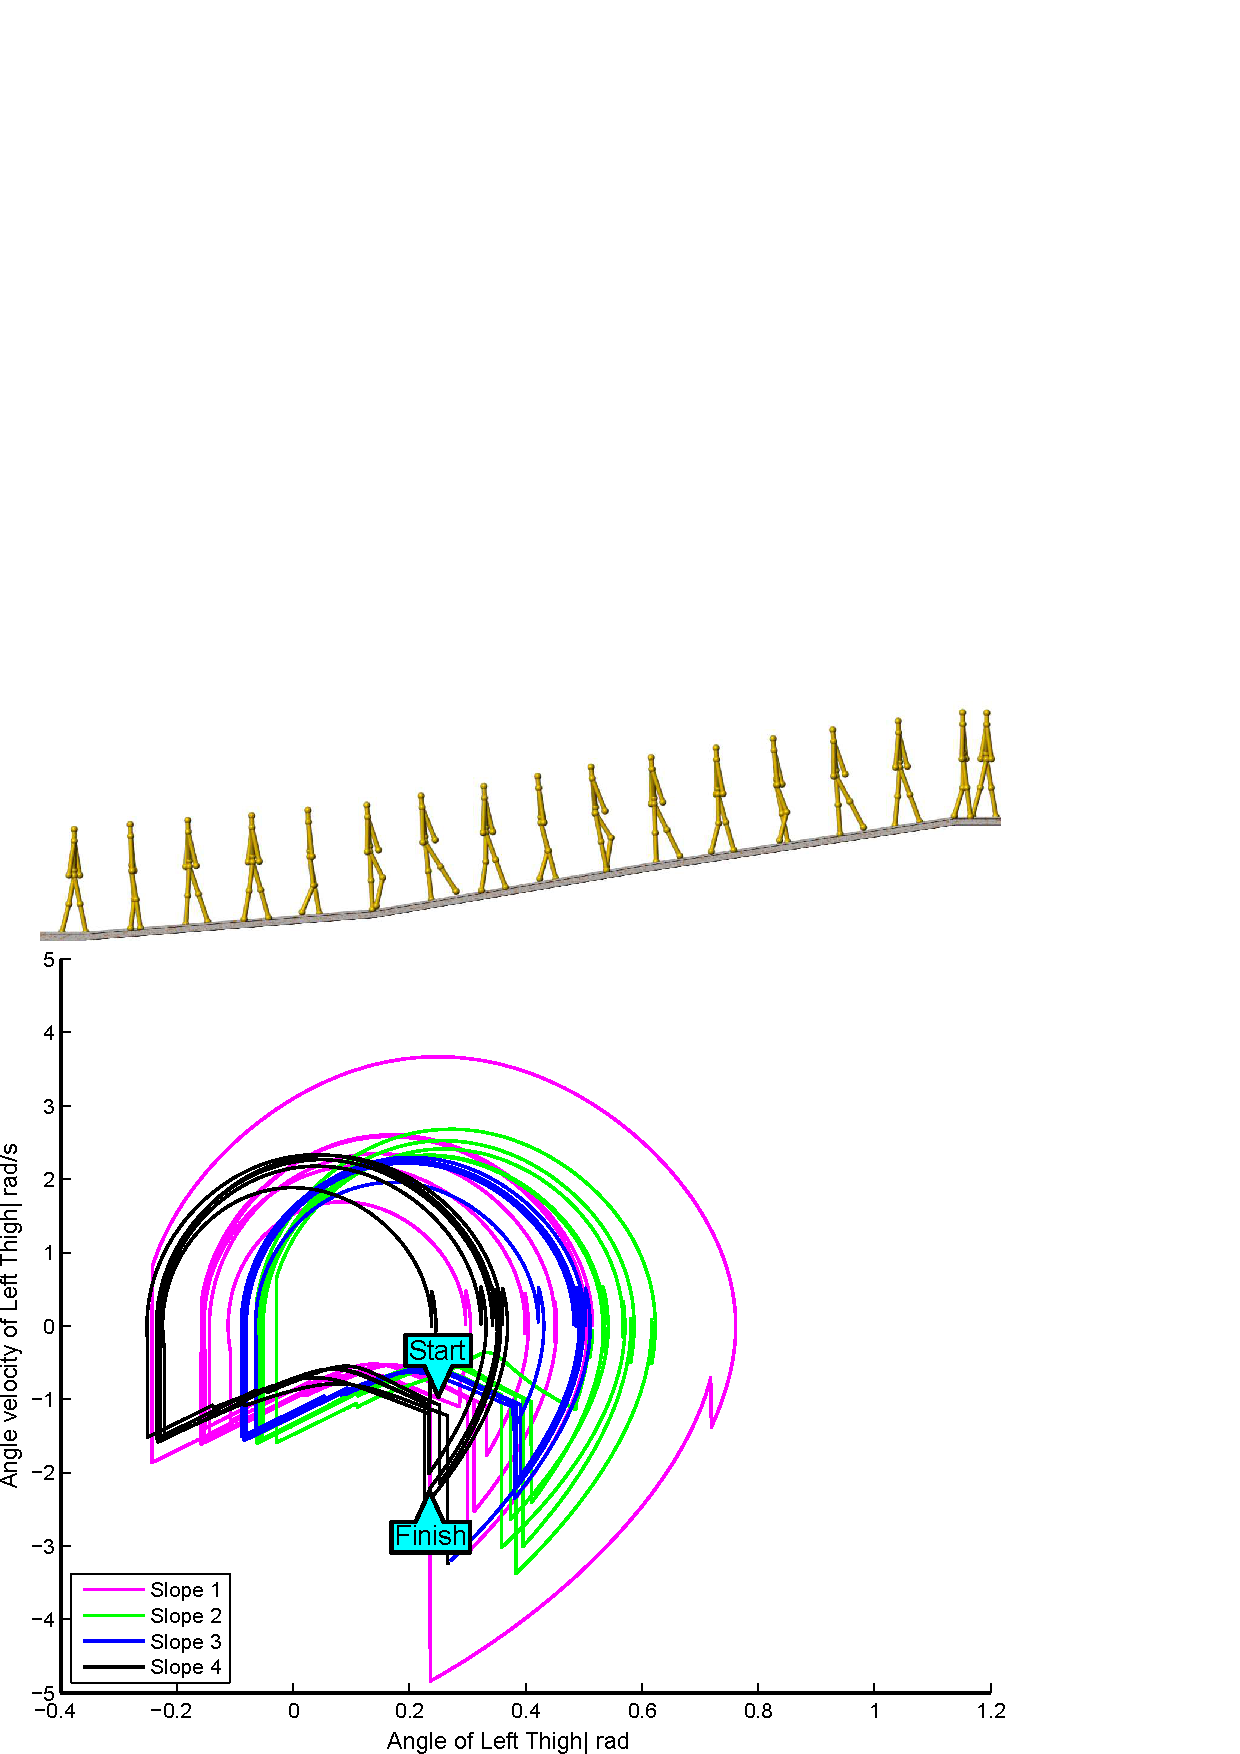
\includegraphics[width=0.7\textwidth]{walk_terrain2}
    \fi
    \caption{Varying Terrain}
    \label{fig:diffterrainphase}
\end{center}
\end{figure}


if the offset action is not enough, we find character can also walk up the slope, just with smaller step size.
Because a smaller offset action is equalivant to walking on the same transform the gait and with the system adaptation of the walking down slop.
In figure 5, we show we adjust the step size by changing the slope action when walking on plane.

\begin{figure}[!htbp]
  \begin{center}
      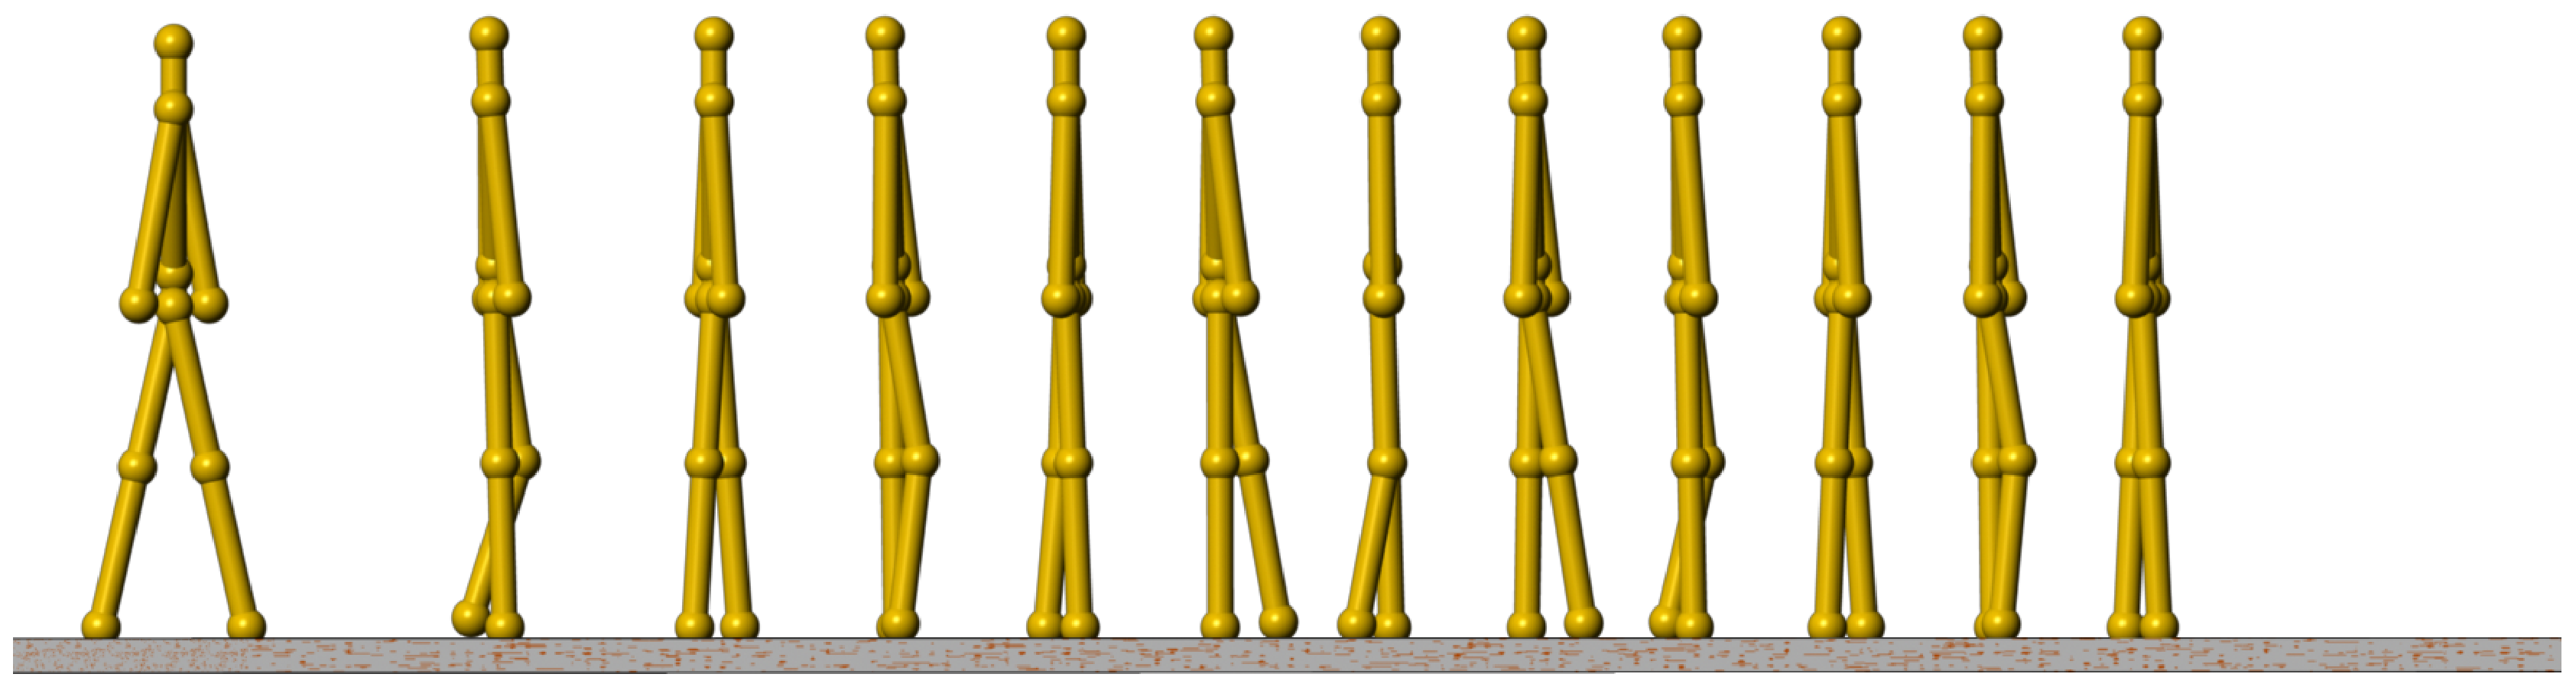
\includegraphics[width=0.7\textwidth]{walking_with_neural}
    \caption{Place Holder1}
    \label{fig:ssp1}
\end{center}
\end{figure}

\begin{figure}[!htbp]
  \begin{center}
      \includegraphics[width=0.7\textwidth]{walking_with_neural}
    \caption{Place Holder2}
    \label{fig:ssp2}
\end{center}
\end{figure}

\begin{figure}[!htbp]
  \begin{center}
      \includegraphics[width=0.7\textwidth]{walking_with_neural}
    \caption{Place Holder3}
    \label{fig:ssp3}
\end{center}
\end{figure}




